%trans 适合幻灯片显示(默认) handout适合讲义
%notes=hide/show/only 适用于笔记。隐藏注释(默认),为pdf screen添加注释,仅产生pdf注释
\documentclass[compress,notes]{beamer}
\usepackage{tikz}
\usepackage{hyperref}
\usepackage{xltxtra} %加入了一些针对xetex的改进,并且加入了\XeTeX 命令来输入漂亮的xetex logo
\usepackage{pdfpages}
\usepackage{listings}


\usepackage{graphicx}
\usepackage{verbatim}
\usetikzlibrary{arrows}
\usepackage{fontspec}
%\setsansfont[Mapping=tex-text,LetterSpace=-1.0]{DejaVu Sans}	 %设置无衬线字体
%\setmainfont[Mapping=tex-text,LetterSpace=-1.0]{WenQuanYi ZenHei} %正文默认字体,衬线字体
%\setmonofont{DejaVu Sans Mono}
\usepackage[CJKchecksingle,normalindentfirst,CJKnumber,BoldFont,SlantFont]{xeCJK}
%\usepackage{XeCJK}



%%Mac OS X
%中文设置
\setCJKmainfont[Scale=1.2,BoldFeatures={FakeBold=2}]{STXihei}
\setCJKmonofont[Scale=1.2,BoldFeatures={FakeBold=2},FakeStretch=1.11686]{STXihei}
\setCJKfamilyfont{usong}{STSong}
\setCJKfamilyfont{ufang}{STFangsong}
\setCJKfamilyfont{ukai}{STKaiti}
\setCJKfamilyfont{uhei}{STHeiti}

\newcommand{\song}{\CJKfamily{usong}}
\newcommand{\fang}{\CJKfamily{ufang}}
\newcommand{\kai}{\CJKfamily{ukai}}
\newcommand{\hei}{\CJKfamily{uhei}}


%%Linux Variant 
%\setsansfont[Mapping=tex-text,BoldFont={sans}]{sans}
%\setmainfont[Mapping=tex-text,BoldFont={sans}]{sans}
\setromanfont{Arial}
%\setromanfont[BoldFont={Apple LiGothic Medium}, BoldFont={Apple LiSung Light}]{STXihei}
%\setmonofont[Scale=0.8]{AppleGothic Regular}
%\setmonofont{Luxi Mono}
\setromanfont{Times New Roman}
%\setromanfont{Arial}
\hypersetup{unicode=true,
 %bookmarks=true,bookmarksnumbered=false,bookmarksopen=false,
 breaklinks=true,pdfborder={0 0 0},colorlinks=true,
 pdfauthor={赵卫国},
 pdfsubject={Linux},
 pdfkeywords={Linux,系统管理,安全,iptables,shell,awk,grep,sed}}
 
\XeTeXlinebreaklocale "zh"  % 表示用中文的断行
\XeTeXlinebreakskip = 0pt plus 1pt % 多一点调整的空间
\renewcommand{\baselinestretch}{1.2} %调整行间距
%%%%%
 %W/o导航条:default, boxes, Bergen, Madrid, Pittsburgh, Rochester
%带树形导航条:Antibes, JuanLesPins, Montpellier。
% 带目录(TOC)的侧边导航条:         Berkeley, PaloAlto, Goettingen, Marburg,  Hannover。
%带微型frame导航条:Berlin, Ilmenau, Dresden, Darmstadt, Frankfurt, Singapore, Szeged。
%带节小节标题: Copenhagen, Luebeck, Malmoe, Warsaw。

%%%定义主题
\usetheme[]{Luebeck}
\usecolortheme{default}
\usefonttheme{default}
\useinnertheme{default}
\useoutertheme{default}


%\useoutertheme[footline=authorinstituetitle,subsection=true]{miniframes}
%\useinnertheme{circles}
%\usefonttheme[only large]{structurebold}
%
%\setbeamercolor{sidebar right}{bg=black!15}
%\setbeamercolor{structure}{fg=blue}
%\setbeamercolor{author}{parent=structure}
%
%\setbeamerfont{title}{series=\normalfont,size=\LARGE}
%\setbeamerfont{title in sidebar}{series=\bfseries}
%\setbeamerfont{author in sidebar}{series=\bfseries}
%\setbeamerfont*{item}{series=}
%\setbeamerfont{frametitle}{size=}
%\setbeamerfont{block title}{size=\small}
%\setbeamerfont{subtitle}{size=\normalsize,series=\normalfont}

\setbeamertemplate{navigation symbols}{} %取消导航条
%\setbeamertemplate{sidebar top}
%{
%  {\usebeamerfont{title in sidebar}%
%    \vskip1.5em%
%    \hskip3pt%
%    \usebeamercolor[fg]{title in sidebar}%
%    \insertshorttitle[width=2cm-6pt,center,respectlinebreaks]\par%
%    \vskip1.25em%
%  }%
%  {%
%    \hskip3pt%
%    \usebeamercolor[fg]{author in sidebar}%
%    \usebeamerfont{author in sidebar}%
%    \insertshortauthor[width=2cm-2pt,center,respectlinebreaks]\par%
%    \vskip1.25em%
%  }%
%  \hbox to2cm{\hss\insertlogo\hss}
%  \vskip1.25em%
%  \insertverticalnavigation{2cm}%
%  \vfill
%}%

%\setbeamertemplate{title page}
%{
%  \vbox{}
%  \vskip1em
% % {\huge Kapitel \insertshortlecture\par}
%  {\usebeamercolor[fg]{title}\usebeamerfont{title}\inserttitle\par}%
%  \vskip0pt plus1filll
%  \leftskip=0pt plus1fill\insertauthor\par
%  \insertinstitute\vskip1em
%}

%\logo{
\includegraphics[width=1cm]{images/rflogo.jpg}}


\title{Linux技术交流}

\author{赵卫国  \\ \textit{wgzhao@kingbase.com.cn}}

\institute[BaseSoft]{工程中心 服务一部}


\date{\today}

% 除掉以下命令的注解 "%" 后, 许多环境都会自动逐段显示
%\beamerdefaultoverlayspecification{<+->}


\graphicspath{{images/}}
%\includeonly{shell-scripting}
\begin{document}
\begin{comment}
	:Title: 培训文档的主控文档
	:Slug: main
	:Tags: 培训 linux
	
	这是所有培训文档的主控文档,用来确定需要包含哪些章节.
	
	| Author: wgzhao,wgzhao@kingbase.com.cn

\end{comment}

\begin{frame}
	\titlepage 
\end{frame}

\begin{frame}[shrink]{Outline}
	\tableofcontents[subsectionstyle=hide]  %[pausesections]
	
\end{frame}

%%公司及产品介绍
\section{公司及产品介绍}
\begin{frame}{公司及产品介绍}
{Red Flag Software}

{Open Soure Software Giant in China}

\end{frame}

\begin{frame}{中科红旗 公司简介}
\begin{itemize}
\item 2000年成立,中科红旗是一家专业从事操作系统及相关网络应用的开发、销售和服务的国际性软件公司,现已成为亚洲最大的Linux 厂商
\item ISO9001质量认证体系
\item 投资方:中国科学院工业与信息化部
\item 连续多年居中国Linux市场第一
\item 连续多年居全球Linux商业桌面产品出货量第一
\item  Asianux全球联盟的领导者
\end{itemize}
\end{frame}

\begin{frame}{中科红旗 2005年中国市场领先\footnote{数据来源:ccw}}
\end{frame}


\begin{frame}{分支机构}
\center \includegraphics[scale=.8]{images/branch.png}
\end{frame}
\section{产品及服务介绍}
\section*{whoami}
\begin{frame}{who am I}
\begin{itemize}
\item Kingbase 新人
\item Linux 重度患者
\item Google 严重依赖者
\item Android 手机用户
\item Mac OS X 伪粉丝
\item Gtalk/Buzz   wgzhao@gmail.com
\item Twitter   @mlsx
\end{itemize}
\end{frame}
%%系统安装,简单的介绍了安装准备事项,安装时的注意事项等
%Author:wgzhao,wgzhao@redflag-linux.com

\section{系统安装}
\begin{frame}[shrink]{Outline}
	\tableofcontents[currentsection]
\end{frame}


%\begin{frame}[t]{Asianux Server 3 安装}
%\begin{columns}
%\column[T]{.5\textwidth}
%	
\includegraphics[scale=.3]{images/axs3-install/box}
%\column[t]{.4\textwidth}
%	\begin{description}
%	\item[kernel] 2.6.18
%	\item [gcc] 4.1.2
%	\item [gtk2] 2.10.4
%	\item [openssh] 4.3p2
%	\item [perl] 5.8.8
%	\item [python] 2.4.3
%	\item [php] 5.1.6	
%	\end{description}
%\end{columns}
%\end{frame}

\subsection{安装前准备}

\begin{frame}{安装前的准备}
\begin{itemize}
\item 原有数据备份
\item 空间规划
\item 多种安装方式

	\begin{itemize}
	\item 光盘直接安装
	\item 硬盘安装,使用iso文件
	\item 网络安装: FTP, HTTP, NFS
	\end{itemize}
\end{itemize}

\end{frame}

\subsection{安装步骤}

\begin{frame}{光盘安装步骤}
\begin{enumerate}
\item BIOS中光驱设置成启动方式
\item 安装方式
	
	\begin{enumerate}
	\item 图形安装
	\item 文本安装
	\end{enumerate}
\item 安装步骤

	\begin{enumerate}
	\item 分区处理
	\item 交换分区 swap 1\textasciitilde{}2倍内存值
	\item 根目录 /
	\item 不同目录安装到不同分区
	\end{enumerate}
\end{enumerate}

\end{frame}


\begin{frame}{光盘启动界面}

\begin{columns}[t]
	\column[t]{.5\textwidth}
	\begin{exampleblock}{插入系统光盘后启动}
	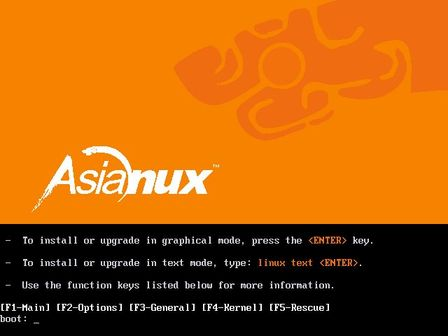
\includegraphics[width=6cm]{images/axs3-install/boot}
	\end{exampleblock}
	
	\pause
	\column[t]{.4\textwidth}
		\begin{exampleblock}{常用的安装内核参数}
			\begin{itemize}
			\item text
			\item acpi=off noapic
			\item dd
			\item rescue
			\end{itemize}
    \end{exampleblock}
\end{columns}
\end{frame}


\begin{frame}{介质检查}

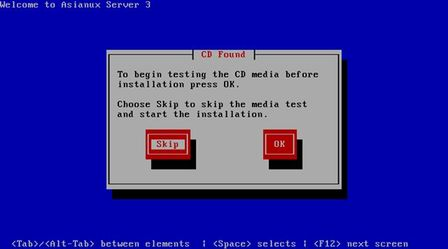
\includegraphics[width=.5\textwidth]{images/axs3-install/disc-check}

\alert{一般可以直接跳过,除非你想确定介质是否完整}

\end{frame}


\begin{frame}{语言选择}
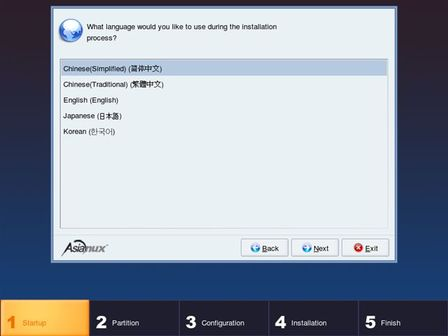
\includegraphics[width=.5\textwidth]{images/axs3-install/lang-choose}
\end{frame}


\begin{frame}{许可协议}

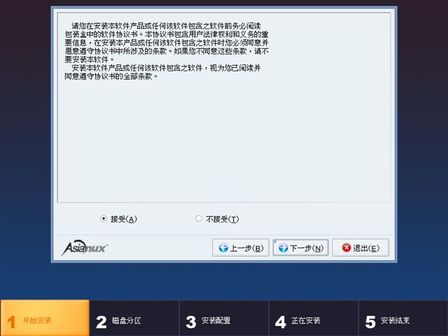
\includegraphics[width=.5\textwidth]{images/axs3-install/eula}
\end{frame}

\begin{frame}{设置键盘}

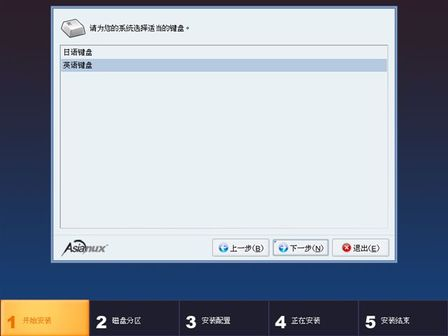
\includegraphics[width=.5\textwidth]{images/axs3-install/keyboard}

\end{frame}
\begin{frame}{选择分区方式}

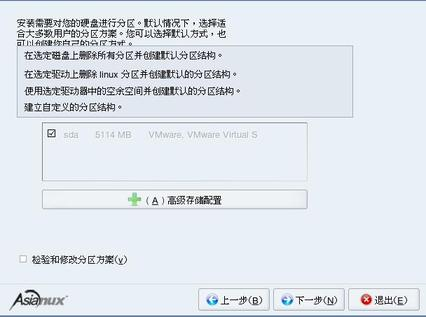
\includegraphics[width=.5\textwidth]{images/axs3-install/partition-method}
\end{frame}

\begin{frame}{设置分区}

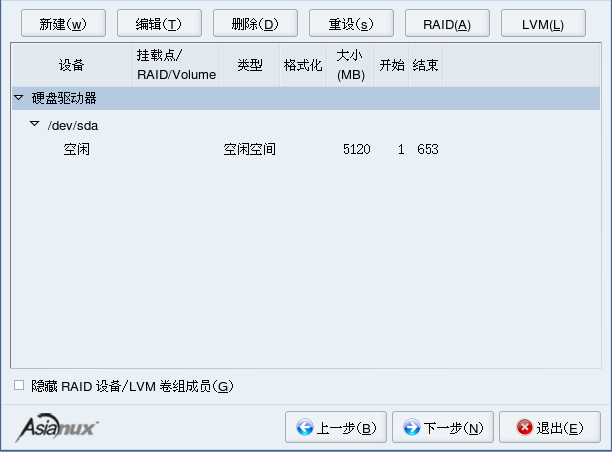
\includegraphics[height=.5\textheight]{images/axs3-install/partition-setup}

\pause
\begin{description}
	\item[/boot] 	 			 \small{引导分区,存放内核以及引导文件}
	\item [/]	根分区,存放操作系统文件
	\item [swap] 交换分区,无挂载点,用作虚拟内存
	\item [/home] 用户分区,存放除root外的用户文件
\end{description}

\end{frame}

\begin{frame}{Linux磁盘及分区识别}
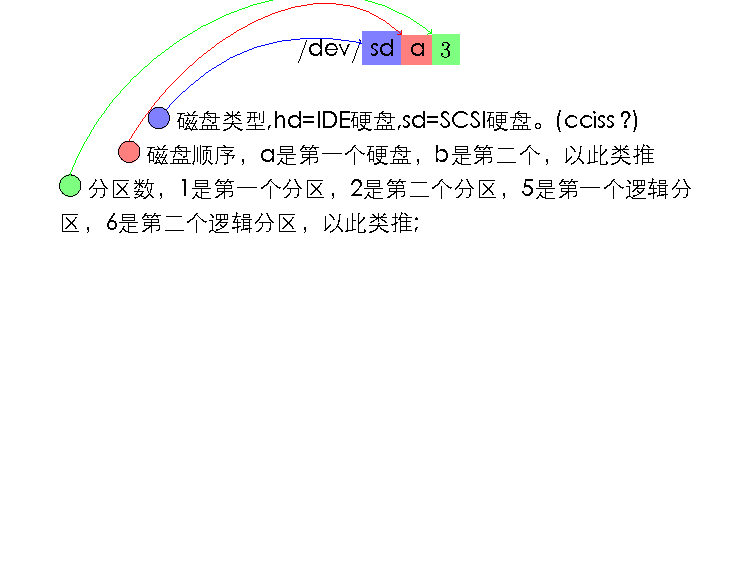
\includegraphics[scale=.8]{disk}
\end{frame}



\begin{frame}[shrink=5]{添加新分区}
	\begin{columns}[t]
		\column{.5\textwidth}
		\begin{exampleblock}{}
			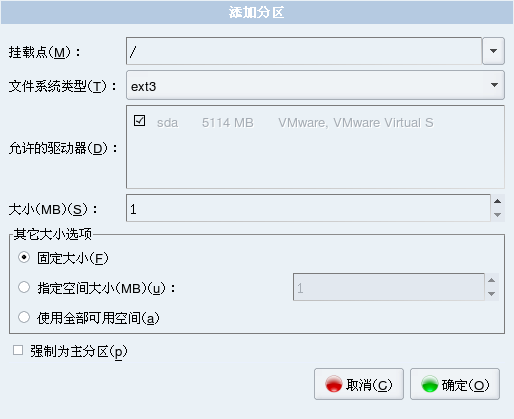
\includegraphics[scale=.35]{images/axs3-install/parition-add}%
		\end{exampleblock}
		
		
		\column[t]{.4\textwidth}
			\begin{exampleblock}{说明}
			\begin{description}
				\item [挂载点] \small{和分区对应起来的目录 /,/home,/var,/etc \ldots}
				\item [文件系统类型] \small{默认使用ext3,交换分区使用swap类型}
				\item [大小] \small{一般情况下/boot 100M,/ 20G,swap 内存的1~2倍}
			\end{description}
			\end{exampleblock}
		\end{columns}

\end{frame}


\begin{frame}{设置根用户口令}

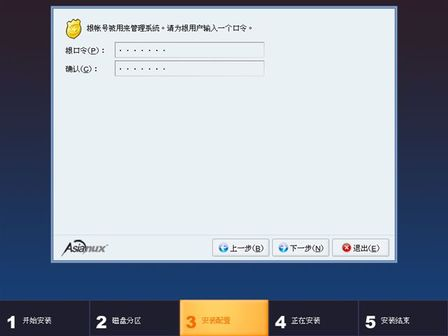
\includegraphics[width=.7\textwidth]{images/axs3-install/password}

\alert{账号是root,这是系统缺省安装后,唯一一个可以登陆的账号}

\end{frame}
\begin{frame}{设置显卡及分辨率}

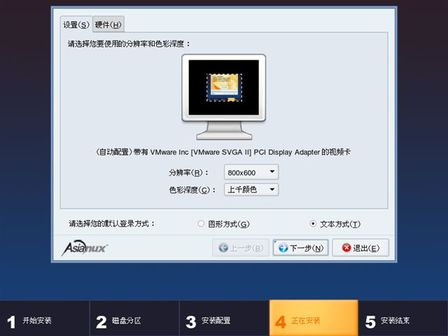
\includegraphics[width=.5\textwidth]{images/axs3-install/resolution}

\end{frame}
\begin{frame}{登录后的界面}

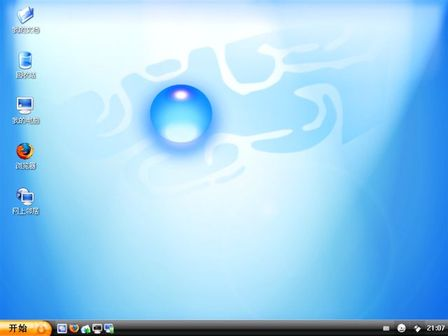
\includegraphics[width=.5\textwidth]{images/axs3-install/desktop}
\end{frame}


%%linux概述
\section{Linux概览}



\begin{frame}[shrink]{Linux概览}
	\tableofcontents[currentsection]
\end{frame}


\subsection{Linux起源}

\begin{frame}{Linux起源}
\begin{itemize}
\item 1984:GNU项目和自由软件基金(Free Software Foundation,FSF)

\begin{itemize}
\item 创建UNIX工具的开源版本
\item 创建通用公共授权(General Public License,GPL)
\end{itemize}

\item 软件必须开源

\item 1991:Linus Torvalds

\begin{itemize}
\item 创建开源,类UNIX的内核,以GPL方式发布
\item 移植一些GNU工具,网上征求援助
\end{itemize}
\item 今天:

\begin{itemize}
\item Linux kernel + GNU 工具 = 完整的,开源的类UNIX的操作系统
\end{itemize}


\end{itemize}

\end{frame}

\subsection{红旗发行版}


\begin{frame}{红旗(RedFlag)发行版}
\begin{itemize}
\item Linux发行版是基于Linux内核的操作系统
\item 红旗服务器操作系统

\begin{itemize}
\item 稳定,经过完整测试的软件
\item 专业的支持服务
\item 针对大型网络的集中管理工具
\end{itemize}
\item Qomo项目

\begin{itemize}
\item 更多,更新的应该程序
\item 社区支持(非红旗官方支持)
\item 针对个人系统
\end{itemize}
\end{itemize}

\end{frame}

\subsection{Linux原则}


\begin{frame}{Linux原则}


\begin{itemize}
\item 所有对象,包括硬件都是文件
\item 配置数据以文本形式保存 
\item 由短小的单目的程序构成 
\item 避免不必要的用户交互 
\item 可使用多个程序合作完成复杂任务
\end{itemize}

\end{frame}

\section{Linux使用基础}


\begin{frame}{Linux使用基础}
%	\begin{exampleblock}{目标}
%	\begin{itemize}
%		\item 登录系统
%		\item 从终端启动X
%		\item 从X访问命令行
%		\item 修改密码
%		\item 理解root特权的性质
%		\item 提升你的权限
%		\item 编辑纯文本文件
%	\end{itemize}
%	\end{exampleblock}
\center 
\includegraphics[scale=.6]{images/tux.png}

\end{frame}

\subsection{登录Linux系统}

\begin{frame}{登录系统}
\begin{itemize}
\item 两种登录屏幕类型:虚拟终端(基于文本)和图形化登录(称为显示管理器)
\item 使用登录帐号和密码登录
\item 每一个用户都有自己的主目录用来保存个人文件
\end{itemize}

\end{frame}

\subsection{虚拟终端和图形界面切换}


\begin{frame}{虚拟终端和图形界面切换}
\begin{itemize}
\item 通常Linux运行6个虚拟终端和一个图形终端
\item 在虚拟终端之间切换,按下:\\
Ctrl+Alt+F\emph{{[}1 - 6{]}}
\item 访问图形终端,按下:Ctrl+Alt+F7
\end{itemize}

\end{frame}

\subsection{改变密码}


\begin{frame}{改变密码 }
\begin{itemize}
\item 密码控制访问系统

\begin{itemize}
\item 首次登录时应该修改密码
\item 此后,要经常修改密码
\item 选择难于猜测的字符串作为密码
\end{itemize}
\item 图形下:
\item 终端下:passwd
\end{itemize}

\end{frame}

\subsection{root账户}


\begin{frame}{root账户}
\begin{itemize}
\item root账户:特殊的管理员帐号

\begin{itemize}
\item 也被称为超级用户(superuser)
\item root有着完全控制系统和彻底摧毁系统的能力
\end{itemize}
\item 如无必要,不要使用root登录
\end{itemize}

\end{frame}

\subsection{改变身份}


\begin{frame}{改变身份}
\begin{itemize}
\item su - 为root帐号创建新的shell环境
\item sudo \emph{command} 用root账户运行命令

\begin{itemize}
\item 需要先前配置/etc/sudoers
\end{itemize}
\item id 显示当前用户的信息
\end{itemize}

\end{frame}

\section{运行命令及获取帮助}


\begin{frame}{运行命令和获取帮助}

目标:
\begin{itemize}
\item 在提示符下执行命令
\item 解释某些简单命令的使用帮助摘要
\item 学会如何使用系统内置的帮助资源
\end{itemize}

\end{frame}

\subsection{运行命令}


\begin{frame}{运行命令}
\begin{itemize}
\item 运行的命令一般是下面的语法:

\begin{itemize}
\item command \textit{options} \textit{arguments}
\end{itemize}
\item 每一项用空格隔开
\item Options 可以修改命令的行为

\begin{itemize}
\item 单字母选项一般用-表示,可以每一个选项单独给出,也可以联合
\item -a -b -c or -abc
\item 完整单词的选项一般用--表示
\item -{}-help -{}-usage
\end{itemize}
\item Arguments 可以是命令需要的文件名或者其他数据
\item 一行中的多个命令可以使用 ; 分隔
\end{itemize}

\end{frame}

\subsection{获取帮助}


\begin{frame}{获取帮助}
\begin{itemize}
\item 不必试着记住所有的指令及用法
\item 多层帮助

\begin{itemize}
\item whatis
\item \textit{command} -{}-help
\item man , info
\item /usr/share/doc
\item 红旗文档
\end{itemize}
\end{itemize}
\end{frame}


\begin{frame}{whatis命令}
\begin{itemize}
\item 显示一个命令的简短描述
\item 使用的数据库每日更新
\item 一般情况下,系统刚安装后无效
\item \$ whatis cal\\
cal (1) - displays a calendar and the date of easter
\end{itemize}
\end{frame}


\begin{frame}[fragile]{-{}-help 选项}
\begin{itemize}
\item 显示用法摘要和参数列表
\item 大部分命令都有此参数
\item  
	\begin{verbatim}
	$mount --help
	
	Usage: mount -V : print version
		mount -h : print this help
		mount : list mounted filesystems	
		mount -l : idem, including volume labels
	\end{verbatim}
	\ldots{} \ldots{}

\end{itemize}
\end{frame}

\begin{frame}{阅读用法摘要}
\begin{itemize}
\item 通过-{}-help,man和其他方式打印出用法摘要
\item 用于描述命令的语法
	\begin{itemize}
		\item \emph{[ {} ]} 里的参数表示可选
		\item {<} {>}或者大写的参数表示是变量
		\item 文本后接 \ldots{} 的表示列表重复
		\item $x | y | z$ 表示“x或y或z”
		\item -abc 意思是-a,-b,-c的任意混合
	\end{itemize}
\end{itemize}
\end{frame}

%%\part{Linux系统管理}
%\section{用户管理}

%

%
%\subsection{增加用户}
%
%
%\begin{frame}{增加用户帐号}
%\begin{itemize}
%	\item 最通常做法是执行useradd指令
%	
%	\begin{itemize}
%		\item useradd \emph{{[}options{]} username}
%	\end{itemize}
%	\item 运行useradd等价于
%	
%		\begin{itemize}
%			\item 编辑/etc/\{passwd,shadow,group,gshadow\}
%			\item 创建和填充用户的主目录(/etc/skel)
%			\item 设置许可和所有权
%		\end{itemize}
%	\item 使用passwd设置密码
%	\item 用newusers批处理增加帐号
%\end{itemize}
%
%\end{frame} 
%
%
%\begin{frame}{用户私有组}
%\begin{itemize}
%\item 用户帐号创建时,一个同名的私有组也同时创建
%
%\begin{itemize}
%\item 用户默认属于这个私有组
%\item 用户的新文件都属于这个组
%\end{itemize}
%\item 好处:防止新文件属于公共组,私密考虑
%\item 缺点:有鼓励设置文件为全局可读的倾向
%\end{itemize}
%
%\end{frame} 
%\begin{frame}{修改/删除用户帐号}
%\begin{itemize}
%\item 改变/etc/passwd文件的一些项值,你可以
%
%\begin{itemize}
%\item 手工编辑该文件
%\item 使用 usermod \emph{{[}options{]} username}
%\end{itemize}
%\item 删除一个帐号可以用以下方法之一
%
%\begin{itemize}
%\item 手工删除/etc/\{passwd,shadow,group,gshadow\},/var/spool/mail等文件的用户信息
%\item 使用 userdel \emph{{[} -r {]} username}
%\end{itemize}
%\end{itemize}
%
%\end{frame} 
%\begin{frame}{管理用户组}
%\begin{itemize}
%\item 本质上是在/etc/\{group,gshadow\}文件中增加或者修改条目信息
%
%\begin{itemize}
%\item groupadd
%\item groupmod
%\item groupdel
%\end{itemize}
%\end{itemize}
%
%\end{frame} 
%\begin{frame}{密码和时效性策略}
%\begin{itemize}
%\item 缺省情况下,密码不过期
%\item 强制密码过期是安全策略的一部分
%\item 通过/etc/login.defs修改缺省的过期设置
%\item 通过chage命令可以修改已有账户的密码期限
%
%\begin{itemize}
%\item chage \emph{{[}options{]} username}
%\end{itemize}
%\end{itemize}
%
%\end{frame} 
%\begin{frame}{切换账户}
%\begin{itemize}
%\item 可以在不注销的情况下,随时切换到其他已有账户环境下
%\item 语法
%
%\begin{itemize}
%\item su {[} - {]} {[} user {]}
%\item su {[} - {]} {[} user {]} -c \emph{command}
%\end{itemize}
%\item 允许当前账户临时变成另外一个账户,缺省是变成root
%\item -,表示创建新的shell环境
%\end{itemize}
%\end{frame} 
%\subsection{特殊许可}
%
%
%
%\begin{frame}{SUID/SGID可执行程序}
%\begin{itemize}
%\item 普通用户如何修改其密码?
%\item 某一个账户运行的进程限制在当前账户的权限上下文环境里
%\item SUID/SGID位的设置,可以使得该程序被执行时,获得的不是程序发起账户而是文件所有者的上下文环境
%\item /bin/mount,/usr/bin/passwd,etc
%\end{itemize}
%
%\end{frame} 
%\begin{frame}{SGID目录}
%
%
%\begin{itemize}
%\item 用来创建协同工作目录
%\item 通常情况下,在目录下创建的文件属于该账户的缺省组
%\item 但是在有SGID位设置的目录下,创建的文件却和该目录属于同一个组
%\item \$ ls -ld a\\
%drwxrw\alert{s}rwx 2 wgzhao wgzhao 4096 2009-10-16 11:27 \\
%\$ ls -l a
%
%
%total 0
%
%
%-rw-r--r-- 1 oracle wgzhao 0 2009-10-16 11:27 oracle
%
%
%-rw-r--r-- 1 wgzhao wgzhao 0 2009-10-16 11:27 wgzhao
%
%\end{itemize}
%
%\end{frame} 
%\begin{frame}{粘滞位 stickly bit}
%
%
%\begin{itemize}
%\item 通常情况下,如果账户对某一个目录有写的许可,就意味着他能删除该目录下的任何文件,而不用考虑文件本身的许可
%\item 但是设置粘滞位后,账户就只能删除属于自己的文件
%\item ls -ld /tmp\\
%drwxrwxrw\alert{t} 17 root root 24576 2009-10-16 11:36 /tmp
%\end{itemize}
%\end{frame} 
%\subsection{实验}
%
%
%
%\begin{frame}{实验I:创建组和用户}
%
%
%\begin{description}
%\item [{场景:}] 你需要为公司不同的部门设置不同的组。同时,你也需要为每一个部门的职员设置帐号
%\item [{要求:}] 系统用户eva和basten在sales组;katherine和lily在hr组;john和crix在web组;manager在sales,hr和web组
%\end{description}
%提示:
%\begin{enumerate}
%\item 确保所有新创建的用户可以创建组可写文件
%\item 设定GID
%\item 私有组,辅助组
%\end{enumerate}
%
%\end{frame} 
%\begin{frame}{实验II:设置共享目录}
%
%
%\begin{description}
%\item [{场景:}] 接上一个场景,你为每一个部门创建的组,同时也需要一个共享目录。\\
%它允许每一个部门内职员共享文件,但是防止其他部门职员修改,甚至看到文件
%\item [{要求:}] 每一个部门的共享目录仅允许部门内职员帐号进入或者在目录内创建,查看和修改文件
%\end{description}
%提示:
%\begin{enumerate}
%\item 创建/depts目录以及sales,hr和web子目录
%\item 设置每一个目录的组所有者
%\item 设置相关权限
%\end{enumerate}
%\end{frame} 


\section{文件系统管理}
\begin{frame}{系统管理}
	\tableofcontents[currentsection]
\end{frame} 

%\begin{frame}{文件系统}
%目标
%\begin{itemize}
%\item 理解文件系统层次结构
%\item 管理交换分区
%\item 增加新的设备于分区
%\item 挂载NFS文件系统
%\end{itemize}
%
%\end{frame} 

%\begin{frame}{概览:增加新文件系统}
%
%要添加一个新的文件系统到系统中,遵循下列步骤:
%\begin{enumerate}
%\item 识别设备
%\item 对设备进行分区(如有必要)
%\item 创建文件系统
%\item 标识文件系统,便于管理(可选)
%\item 在/etc/fstab增加新条目(可选)
%\item 挂载新的文件系统
%\end{enumerate}
%\end{frame} 

\subsection{设备与分区}

\begin{frame}{磁盘分区}
\begin{itemize}
\item 内核支持的最大分区数:

\begin{itemize}
\item IDE设备,63个
\item SCSI设备,15个
\end{itemize}
\item 为什么要分区?

\begin{itemize}
\item 容量
\item 性能
\item 配额
\item 恢复
\end{itemize}
\end{itemize}

\end{frame} 
\begin{frame}{管理分区}
\begin{itemize}
\item 使用下列程序来创建和管理分区:

\begin{itemize}
\item fdisk
\item sfdisk
\item GNU parted 高级分区处理
\end{itemize}
\item partprobe 
\end{itemize}

\end{frame} 
\begin{frame}{fdisk}
\begin{itemize}
\item 查看和管理分区表
\item 从命令行列出分区表

\begin{itemize}
\item fdisk -l
\end{itemize}
\item 交互模式管理分区表

\begin{itemize}
\item fdisk \emph{/dev/sda}
\end{itemize}
\item partprobe
\item cat /proc/partitions
\end{itemize}
\end{frame} 

\subsection{文件系统创建与调整}

\begin{frame}{创建文件系统}
\begin{itemize}
\item mkfs
\item mkfs.ext2,mkfs.ext3,mkfs.ext4,mkfs.msdos
\item 特殊文件系统工具可以直接调用

\begin{itemize}
\item mke2fs \emph{{[} options {]} device}
\end{itemize}
\end{itemize}

\end{frame} 
\begin{frame}{文件系统标签(label)}
\begin{itemize}
\item 引用设备的另一方法
\item 设备独立性,不受特定设备名约束

\begin{itemize}
\item e2label \emph{special\_dev\_file {[} fslabel {]}}
\item mount \emph{{[} options {]}} LABEL=\emph{fslabel mount\_point}
\end{itemize}
\item blkid 可以查看所有设备的标签,文件系统类型以及UUID号 
\begin{exampleblock}{}
\# blkid -o value -s UUID /dev/sda2 \\
f252a71d-cf7d-4166-8315-cda1e217a08c
\end{exampleblock}
\end{itemize}
\end{frame} 


\begin{frame}{tune2fs}
\begin{itemize}
\item tune2fs 用来调整文件系统参数

\begin{itemize}
\item 保留块,缺省是5\%
\item 缺省挂载选项,缺省是defaults
\item fsck的频率,缺省是挂载次数30次,时长180天
\end{itemize}
\item dumpe2fs 查看当前设置
\end{itemize}
\end{frame} 

\subsection{挂载}

\begin{frame}{挂载点和/etc/fstab}
\begin{itemize}
\item 系统层次结构的配置文件
\item 被mount,fsck及其他工具使用
\item 系统重启后还能维持层次结构
\item /etc/fstab中的设备域可以用标签(label)替代,推荐这样做!
\item mount -a 能挂载所有在/etc/fstab里设定的文件系统,有noauto标志除外
\end{itemize}

\end{frame} 
\begin{frame}{用mount挂载文件系统}
\begin{itemize}
\item mount \emph{{[} options {]}} \emph{device mount\_point}

\begin{itemize}
\item -t 指定文件系统类型,一般不需要
\item -o 挂载选项,缺省挂载选项为
\item rw,suid,dev,exec,acl,async
\end{itemize}
\end{itemize}

\end{frame} 
\begin{frame}{卸载文件系统}
\begin{itemize}
\item umount \emph{{[} options {]} device | mount\_point}
\item 不能卸载仍在被使用的文件系统

\begin{itemize}
\item 使用fuser检查或杀死进程
\end{itemize}
\item 使用remount选项可以在自动改变挂载选项

\begin{itemize}
\item mount -o remount,ro /dev/sda1 /data
\end{itemize}
\end{itemize}
\end{frame} 

\subsection{特定文件系统}

\begin{frame}{交换空间 swap}
\begin{itemize}
\item 交换空间是对物理内存的有效补充
\item 基本设置步骤:

\begin{itemize}
\item 创建一个交换分区或者文件
\item 使用mkswap写入分区特征信息
\item 在/etc/fstab增加正确的条目
\item 使用swapon -a激活交换空间
\end{itemize}
\end{itemize}

\end{frame} 
\begin{frame}{挂载NFS文件系统}
\begin{itemize}
\item 把远程的目录当作本地文件系统来挂载使用
\item /etc/fstab支持NFS挂载配置
\item 通过/etc/init.d/netfs可以自动挂载NFS
\item 手工挂载方式

\begin{itemize}
\item mkdir /mnt/srv1-nfs
\item mount -t nfs \emph{srv1:/data/shared /mnt/srv1-nfs}
\end{itemize}
\end{itemize}
\end{frame} 

%\subsection{实验}
%
%
%
%\begin{frame}{实验 I: 创建新的文件系统}
%\begin{description}
%\item [{场景:}] 新的应用程序需要安装到/opt目录。基于恢复的原因,/opt需要成为单独的分区,新的/opt分区重启后依然有效
%\item [{要求:}] 系统提供独立分区挂载到/opt
%\end{description}
%提示:
%\begin{enumerate}
%\item 创建新的分区(fdisk/parted)
%\item 创建文件系统(mkfs,mke2fs)
%\item 修改/etc/fstab
%\end{enumerate}
%
%\end{frame} 
%\begin{frame}{实验II:创建新的交换空间}
%\begin{description}
%\item [{场景:}] 系统目前的交换分区已经不够用,需要增加交换分区,但是不能影响现有的其他分区。所有的交换分区都应该在系统重启后仍然激活
%\item [{要求:}] 给系统增加一个交换分区
%\end{description}
%提示:
%\begin{enumerate}
%\item 创建新分区
%\item 创建交换系统
%\item 激活测试
%\item 持久化
%\end{enumerate}
%
%\end{frame} 
%\begin{frame}{实验III:挂载实践}
%\begin{description}
%\item [{要求:}] 使用合适的挂载参数来完成下面的需求
%
%\begin{itemize}
%\item 禁止可执行访问
%\item 挂载一个文件系统镜像
%\item 挂载非Linux文件系统
%\item 禁止访问时间更新
%\item 设置一个挂载别名
%\end{itemize}
%\end{description}
%\end{frame} 


\section{包管理}

\begin{frame}{包管理}

%目标:
%\begin{itemize}
%\item 安装和删除RPM包
%\item 查询包和校验状态
%\item 使用yum管理包
%\item 了解yum和rpm的关系
%\item 利用yum来在线更新包
%\item 制作RPM包
%\end{itemize}
\tableofcontents[currentsection]
\end{frame} 

\subsection{RPM包管理}

\begin{frame}{RPM包管理}
\begin{itemize}
\item RPM(\alert{R}edhat \alert{P}ackages \alert{M}anager) 组件:

\begin{itemize}
\item 本地数据库
\item rpm和相关可执行程序
\item rpm前端程序如yum
\item 包文件
\end{itemize}
\item 基本功能:

\begin{itemize}
\item 安装/删除
\item 查询
\item 校验
\end{itemize}
\end{itemize}
\end{frame} 

\subsection{安装和删除软件}



\begin{frame}{安装和删除软件}
\begin{itemize}
\item 基本rpm指令参数:

\begin{itemize}
\item 安装 rpm -i,--install
\item 升级 rpm -U, --upgrade
\item 刷新 rpm -F,--freshen
\item 
\item 删除 rpm -e,--erase
\end{itemize}
\item 输出选项: -v,-h
\item URL支持: ftp://,http://
\end{itemize}
\end{frame} 

\subsection{更新内核RPM包}


\begin{frame}{更新内核RPM包}
\begin{itemize}
\item 真的需要更新内核?
\item \alert{不要使用rpm -U,rpm -F方式更新内核}

\begin{itemize}
\item rpm -ivh kernel-version.arch.rpm
\item 启动新内核,测试
\item 如果新内核有问题,回退到旧内核
\item 如果没有问题,删除旧内核 rpm -e kernel-oldversion
\end{itemize}
\end{itemize}
\end{frame} 

\subsection{rpm指令}



\begin{frame}{rpm查询}
\begin{itemize}
\item 语法:

\begin{itemize}
\item rpm -q what\_packages what\_information
\end{itemize}
\item 查询已安装选项

\begin{itemize}
\item rpm -qa 列出已经安装的包
\item rpm -qf filename 查询filename属于那个包
\item rpm -qi pkg 显示包pkg的一般信息
\item rpm -ql pkg 列出包pkg安装的文件
\end{itemize}
\item 查询未安装包选项

\begin{itemize}
\item rpm -qip pkg.i386.rpm 显示一般信息
\item rpm -qlp pkg.i36.rpm 列出包含的文件
\end{itemize}
\end{itemize}

\end{frame} 
\begin{frame}{rpm校验}
\begin{itemize}
\item 已安装的rpm包校验

\begin{itemize}
\item rpm -V pkg\_name
\item rpm -Vp pkg\_name.i386.rpm
\item rpm -Va
\end{itemize}
\item 包安装前校验签名

\begin{itemize}
\item rpm --import RPM-GPG-KEY
\item rpm -K pkg\_name.i386.rpm
\end{itemize}
\end{itemize}

\end{frame} 
\begin{frame}{关于yum}
\begin{itemize}
\item rpm的前端程序

\begin{itemize}
\item 旨在解决包依赖关系
\item 能跨软件源找到包
\end{itemize}
\end{itemize}

\end{frame} 
\begin{frame}{使用yum}
\begin{itemize}
\item 安装/删除/更新

\begin{itemize}
\item yum install \emph{package} \ldots{}
\item yum remove \emph{package} \ldots{}
\item yum update {[} \emph{package} \ldots{} {]}
\end{itemize}
\item 搜索包/文件
\item 搜索包

\begin{itemize}
\item yum search \emph{searchterm}
\item yum list (all|available|extras|installed|recent|updates)
\item yum info \emph{packagename}
\end{itemize}
\item 搜索文件

\begin{itemize}
\item yum whatprovides \emph{filename}
\end{itemize}
\end{itemize}
\end{frame} 

%\begin{frame}{配置其他软件库(Repository)}
%\begin{itemize}
%\item 给库创建一个文件,保存在/etc/yum.repos.d/目录,后缀为.repo
%\item 必要的一些信息
%
%\begin{itemize}
%\item {[}\emph{repo-name}{]}
%\item name= \emph{A nice description}
%\item baseurl = \emph{http://yourserver.com/path/to/repo}
%\item enabled=1
%\item gpgcheck=1
%\end{itemize}
%\item 仓库信息缓存到本地,使用下面的命令清除:
%
%\begin{itemize}
%\item yum clean dbcache | all
%\end{itemize}
%\end{itemize}
%
%\end{frame} 
%\begin{frame}{创建自己的软件库}
%\begin{itemize}
%\item 创建目录,将软件包存放到此
%\item 使得该目录能够通过http/ftp 访问
%\item 安装 createrepo RPM包
%\item 运行 createrepo -v \emph{/package/directory}
%\item 将创建 repodata 子目录以及其他必要的支持文件
%\end{itemize}
%\end{frame} 

\subsection{制作RPM包}

\begin{frame}{制作RPM包}
在目前的Linux环境下,要安装新软件,通常有两种方式:一是使用源码安装;二是使用rpm软件包。使用源码安装可以让用户了解编译过程,及定制一些模块,和修改编译参数,但其工作量通常都很大,而且要求用户有足够的计算机知识。而rpm软件包方式则相对来说比较简单,也易于管理和升级。所以,当前Linux发行版的前十中,有八个都是使用基于二进制软件包方式的(deb和rpm格式可以互转)。
\end{frame}

\begin{frame}{目录准备}
/usr/src/asianux/ \\
|-- BUILD   ---编译时的工作目录,包括解压和make都会放到这里 \\
|-- RPMS   ---根据硬件平台的不同,存放最后生成的RPM软件包 \\
|-- SOURCES ---存放源码包的地方,一般带压缩的tar包 \\
|-- SPECS ---存放编译RPM时的.spec脚本 \\
|-- SRPMS ---存放编译好的.src.rpm软件包 \\
\end{frame}

\begin{frame}[plain]{rpm制作流程}
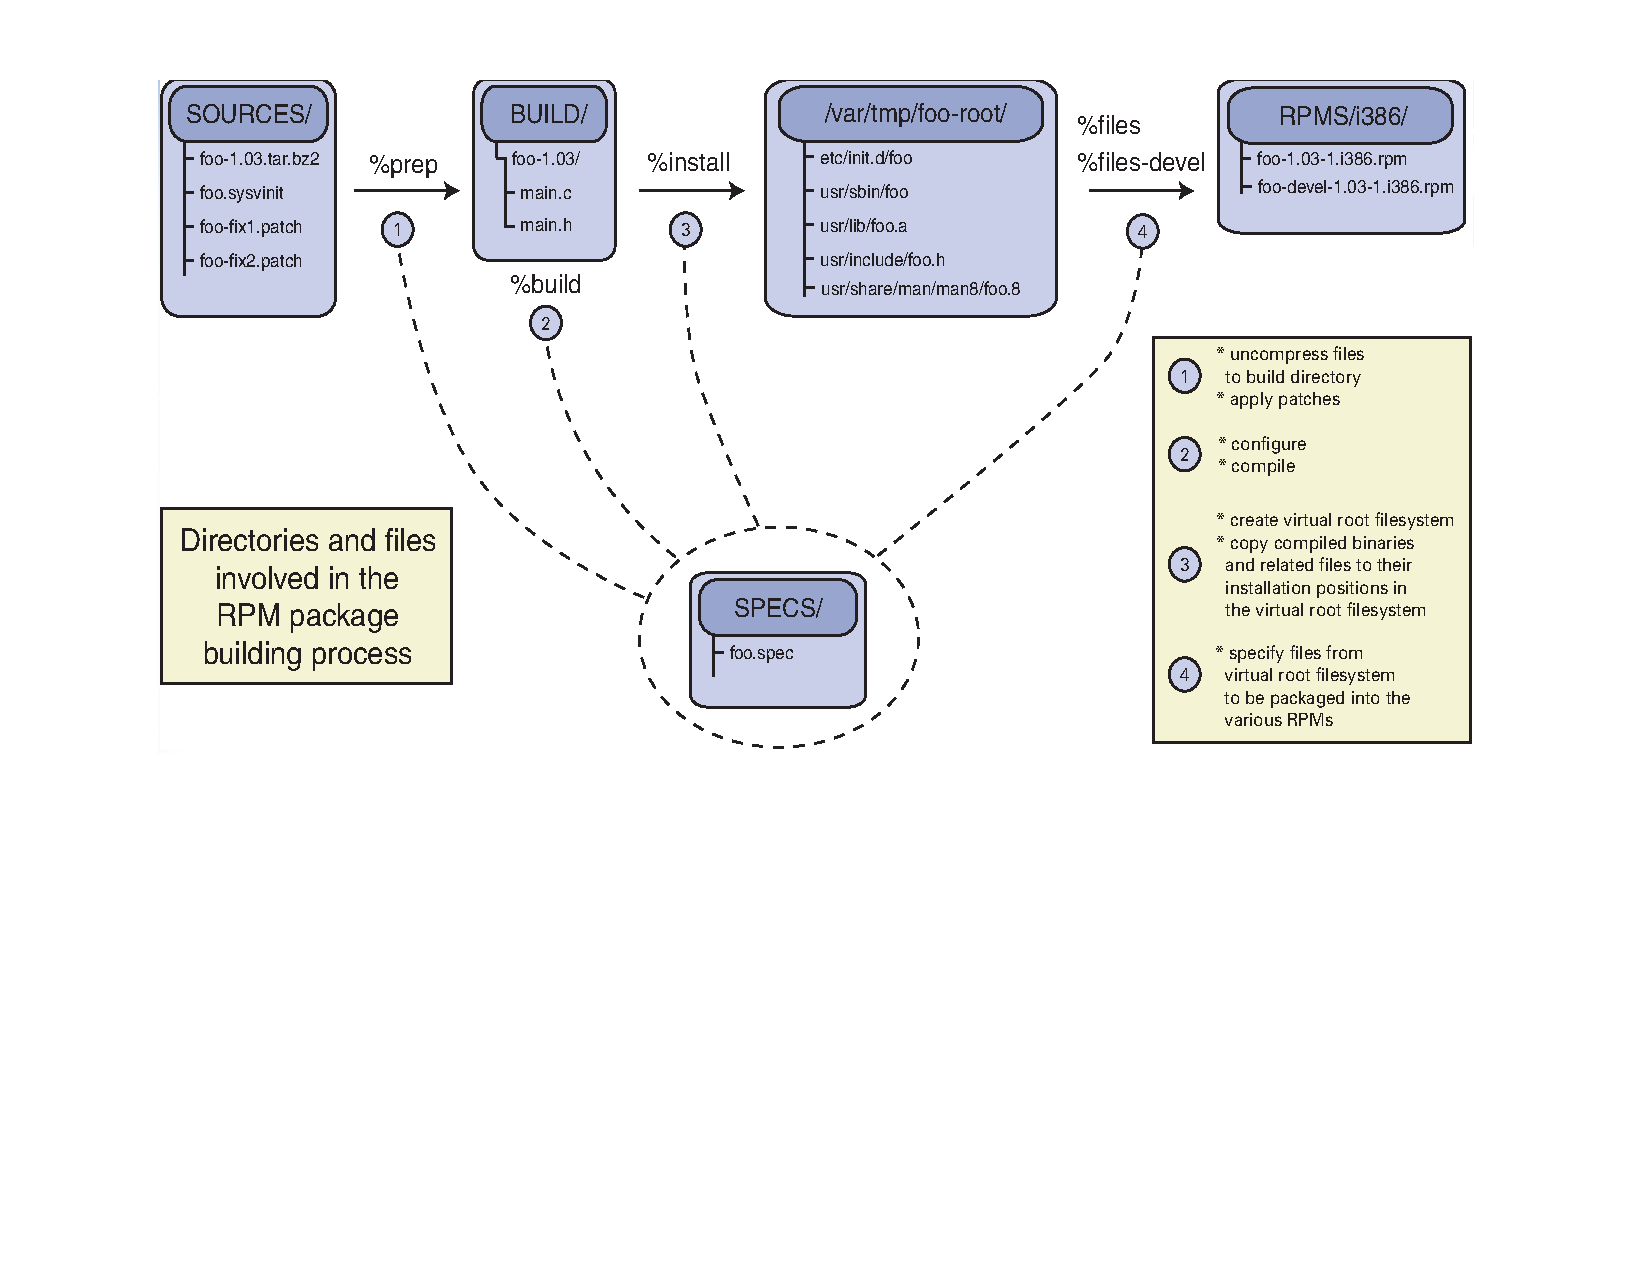
\includegraphics[scale=.5]{rpm-build-flowcharts} \footnote{http://www.gurulabs.com/GURULABS-RPM-LAB/GURULABS-RPM-GUIDE-v1.0.PDF}
\end{frame}

\begin{frame}[fragile]{自定义目录}
\begin{verbatim}
echo "%_topdir $HOME/rpm" >> $HOME/.rpmmacros
mkdir $HOME/rpm
mkdir $HOME/rpm/SOURCES
mkdir $HOME/rpm/SPECS
mkdir $HOME/rpm/BUILD
mkdir $HOME/rpm/SRPMS
mkdir $HOME/rpm/RPMS
mkdir $HOME/rpm/RPMS/i386
echo '%debug_package %{nil}' >> ~/.rpmmacros  
		#does not create debuginfo rpm package
\end{verbatim}
\end{frame}

\begin{frame}{从rpm源代码创建rpm包}
\begin{enumerate}
\item  下载需要的rpm源代码包,后缀一般是src.rpm
\item 执行下面的指令来直接编译: \\
rpmbuild -{}-rebuild foo-<version>.src.rpm
\item 如果编译正常,生成的rpm包放在 \\
/usr/src/asianux/RPMS/目录下
\end{enumerate}
\end{frame}


\begin{frame}{rpmbuild 常用参数}
\begin{description}
\item[-{}-rebuild] 从源代码包编译二进制包
\item[-ba] 从spec文件编译源代码包和二进制包
\item[-bb] 从spec文件仅编译二进制包
\item[-bs] 从spec文件仅编译源代码包
\item[-ta] 从tar包编译源代码和二进制包
\item[-tb] 从tar包仅编译二进制包
\item[-ts] 从tar包仅编译源代码包
\end{description}
注意: \\
这里说的源代码包是指后缀为.src.rpm的包 \\
spec文件说的是后缀为.spec文件 \\
tar包说的是以.tar.gz/.tar.bz2等格式的源代码 \\
二进制包指的是后缀为.rpm的包
\end{frame}

\begin{frame}[fragile,allowframebreaks]{spec文件说明:关键字}
spec文件包括很多关键字,主要有
\begin{description}
\item[Name] 软件包的名字,后面可以使用\%\{name\} 的方式引用
\item[Summary] 软件包的内容摘要
\item[Version] 软件的实际版本号,例如 2.1.4,后面可以用\%\{version\}引用
\item[Release] 发布序列号,比如12,标明第几次打包,后面可用\%\{release\}引用
\item[Group] 软件分组,建议使用标准分组
\item[License] 软件授权方式,GPL,LGPL,BSD,MPL, MIT,$\cdots$
\item[Source] 源代码包,可以带多个用Source1,Source2等源,后面可以用\%\{source1\},\%\{source2\}引用
\item[BuildRoot] 这个是安装或编译时使用的“虚拟目录”,考虑到多用户的环境,一般定义为:\\
\%\{\_tmppath\}/\%\{name\}-\%\{version\}-\%\{release\}-root \\
或 \\
\%\{\_tmppath\}/\%\{name\}-\%\{version\}-\%\{release\}-buildroot-\%(\%\{\_\_id\_u\} -n\} \\
该参数非常重要,因为在生成rpm的过程中,执行make install时就会把软件安装到上述的路径中,在打包的时候,同样依赖“虚拟目录”为“根目录”进行操作。
后面可使用\$RPM\_BUILD\_ROOT 方式引用
\item[URL] 软件的主页
\item[Vendor]发行商或打包组织的信息,例如BaseSoft Co,.Ltd.
\item[Patch] 补丁代码,可以使用Patch1,Patch2等标识多个补丁,后面使用\%patch0 或\%\{patch0\} 引用
\item[Prefix: \%\{\_prefix\}] 这个主要是为了解决今后安装rpm包时,并不一定把软件安装到rpm中打包的目录的情况。这样,必须在这里定义该标识,并在编写\%install脚本的时候引用,才能实现rpm安装时重新指定位置的功能
\item[Prefix: \%\{\_sysconfdir\}] 这个原因和上面的一样,但由于\%\{\_prefix\}指/usr,而对于其他的文件,例如/etc下的配置文件,则需要用\%\{\_sysconfdir\}标识
\item[Build Arch] 指编译的目标处理器架构,noarch标识不指定,但通常都是以/usr/lib/rpm/marcros中的内容为默认值

\item[Requires] 该rpm包所依赖的软件包名称,可以用>=或<=表示大于或小于某一特定版本,例如:\\
libpng-devel >= 1.0.20 zlib \\ 
“>=”号两边需用空格隔开,而不同软件名称也用空格分开
还有例如PreReq、Requires(pre)、Requires(post)、Requires(preun)、Requires(postun)、BuildRequires等都是针对不同阶段的依赖指定 

\item[Provides] 指明本软件一些特定的功能,以便其他rpm识别

\item[Packager] 打包者的信息

\item[\%description] 软件的详细说明
\end{description}

\end{frame}

\begin{frame}[allowframebreaks]{spec文件说明:脚本主体 }
spec脚本的主体中也包括了很多关键字和描述
\begin{description}
\item[\%prep] 预处理脚本
\item[\%setup -n \%\{name\}-\%\{version\}]把源代码解压并放好 \\
通常是从/usr/src/asianux/SOURCES里的包解压到/usr/src/asianux/BUILD/\%\{name\}-\%\{version\}中。
一般用\%setup -c就可以了,但有两种情况:一就是同时编译多个源码包,二就是源码的tar包的名称与解压出来的目录不一致,此时,就需要使用-n参数指定一下了。
\item[\%patch] 打补丁 \\
通常补丁都会一起在源码tar.gz包中,或放到SOURCES目录下。一般参数为:
\%patch -p1 使用前面定义的Patch补丁进行,-p1是忽略patch的第一层目录
\%Patch2 -p1 -b xxx.patch 打上指定的补丁,-b是指生成备份文件

\item[\%configure] 这个不是关键字,而是rpm定义的标准宏命令。意思是执行源代码的configure配置 \\
在/usr/src/asianux/BUILD/\%\{name\}-\%\{version\}目录中进行 ,使用标准写法,会引用/usr/lib/rpm/marcros中定义的参数。

\item[\%build] 开始构建包 \\
在/usr/src/asianux/BUILD/\%\{name\}-\%\{version\}目录中进行make的工作,常见写法: \\
make \%\{?\_smp\_mflags\} OPTIMIZE="\%\{optflags\}" \\
都是一些优化参数,定义在/usr/lib/rpm/marcros中

\item[\%install] 开始把软件安装到虚拟的根目录中
在/usr/src/asianux/BUILD/\%\{name\}-\%\{version\}目录中进行make install的操作。这个很重要,因为如果这里的路径不对的话,则下面\%file中寻找文件的时候就会失败。
\item[\%clean] 清理临时文件
%通常内容为 
%\begin{verbatim}
%[ "$RPM_BUILD_ROOT" != "/" ] && rm -rf "$RPM_BUILD_ROOT"
%rm -rf $RPM_BUILD_DIR/%{name}-%{version}
%\end{verbatim}
%\alert{\$RPM\_BUILD\_ROOT 是指开头定义的BuildRoot,\\ \$RPM\_BUILD\_DIR 通常就是指/usr/src/asianux/BUILD,其中,前面的才是 \%file 需要的。}

\item[\%pre] rpm安装前执行的脚本
\item[\%post] rpm安装后执行的脚本

\item[\%preun] rpm卸载前执行的脚本

\item[\%postun] rpm卸载后执行的脚本

\item[\%files] 定义哪些文件或目录会放入rpm中 \\
\alert{这里会在虚拟根目录下进行,千万不要写绝对路径,而应用宏或变量表示相对路径}
\item[\%defattr(-,root,root)] 指定包装文件的属性,分别是(mode,owner,group),-表示默认值,对文本文件是0644,可执行文件是0755

\item[\%exclude] 列出不想打包到rpm中的文件 \\
\alert{如果指定的文件不存在,也会出错的} 
\item[\%changelog] 变更日志
\end{description}
\end{frame}


\begin{frame}[allowframebreaks]{foobar.spec 简析}
\lstinputlisting{scripts/foobar.spec}
\end{frame}

\begin{frame}{参考资料}
\begin{itemize}
\item \href{http://fedoranews.org/alex/tutorial/rpm/}{RPM Tutorial}
\item \href{http://docs.fedoraproject.org/en-US/Fedora_Draft_Documentation/0.1/html/RPM_Guide/index.html}{Fedora RPM Guide}
\item \href{http://www.gurulabs.com/GURULABS-RPM-LAB/GURULABS-RPM-GUIDE-v1.0.PDF}{Create RPMs}
\item \href{http://docs.fedoraproject.org/en-US/Fedora_Draft_Documentation/0.1/html/RPM_Guide/ch-rpm-programming-python.html} {Programming RPM with Python} 
\end{itemize}
\end{frame}

%\subsection{软件包实验}
%
%
%
%\begin{frame}{实验I:使用RPM}
%\begin{itemize}
%\item 插入第一张光盘,进入到/media/cdrom/Asianux/RPMS目录,完成下面的问题
%
%\begin{enumerate}
%\item 使用rpm -i util-linux来安装util-linux软件包,应该会失败,纠正这个问题
%\item initscripts 包有哪些文件?
%\item pam软件包自安装后是否有过改动,如果有,改动了哪些文件?
%\item /bin/grep 文件是哪个包提供的?
%\item /etc/hosts是那个软件包提供的,为什么?
%\end{enumerate}
%\end{itemize}
%
%\end{frame} 
%\begin{frame}{实验II:连接到软件库}
%\begin{description}
%\item [{场景:}] firefox浏览器没有默认不提供flash的支持,请创建flash软件的仓库,确保能连接到仓库
%\item [{要求:}] 配置包含adobe软件的仓库
%\end{description}
%
%\end{frame} 
%\begin{frame}{实验III:用yum安装新软件}
%\begin{description}
%\item [{要求:}] 使用yum安装flash插件
%\end{description}
%
%\end{frame} 
%\begin{frame}{实验IV:用yum更新软件}
%\begin{description}
%\item [{要求:}] 针对你想要更新的软件包,在网络上找到对应的仓库,并更新
%\end{description}
%\end{frame} 
%\section{网络配置}
%
%
%
%\begin{frame}{网络配置}
%
%目标
%\begin{itemize}
%\item 配置IP接口
%\item 设置路由
%\item 理解名字解析
%\end{itemize}
%\end{frame} 
%
%\subsection{概述}
%
%
%
%\begin{frame}{网络接口}
%\begin{itemize}
%\item 网络配置脚本需要涉及到设备的逻辑名
%
%\begin{itemize}
%\item 以太网:eth0,eth1 \ldots{}
%\item 拨号:ppp0,ppp1 \ldots{}
%\item 回路:lo
%\end{itemize}
%\item 显示网络接口
%
%\begin{itemize}
%\item ifconfig -a
%\item ip link {[} show {]}
%\end{itemize}
%\end{itemize}
%
%\end{frame} 
%\begin{frame}{驱动选择}
%\begin{itemize}
%\item 所有的网卡驱动都编译成内核模块
%\item /etc/modprobe.conf 将网卡逻辑名映射到特性的内核模块上
%
%\begin{itemize}
%\item alias eth0 bnx2
%\end{itemize}
%\item 通过/etc/sysconfig/network-scripts/ifcfg-eth0的配置也能选定特定网卡
%
%\begin{itemize}
%\item HWADDR=00:12:34:00:00:00
%\end{itemize}
%\end{itemize}
%
%\end{frame} 
%\begin{frame}{速率和双工设置}
%\begin{itemize}
%\item 缺省情况下,速率和双工配置是自动协商的
%\item 速率,双工与设备或者网络不匹配会导致通讯的断断续续
%\item 可以手工设定参数
%
%\begin{itemize}
%\item ethtool
%\item ifcfg-ethX里设置ETHTOOL\_OPTS参数
%\item 如果内核模块支持,在/etc/modprobe.conf里加入options或install 选项
%\end{itemize}
%\end{itemize}
%\end{frame} 
%
%\subsection{IPv4配置}
%
%
%
%\begin{frame}{IPv4地址}
%
%查看配置
%\begin{itemize}
%\item ifconfig
%\item ip addr {[} show {]}
%\end{itemize}
%
%\end{frame} 
%\begin{frame}{动态IPv4配置}
%\begin{itemize}
%\item 配置文件
%
%\begin{itemize}
%\item /etc/sysconfig/network-scripts/ifcfg-\emph{ethX}
%\item BOOTPROTO=dhcp 表示动态配置IPv4地址
%\end{itemize}
%\end{itemize}
%
%\begin{itemize}
%\item 使用ifdown \emph{device};ifup \emph{device} 应用新的配置
%\end{itemize}
%
%\end{frame} 
%\begin{frame}{静态IPv4配置}
%\begin{itemize}
%\item 配置文件
%
%\begin{itemize}
%\item /etc/sysconfig/network-scripts/ifcfg-\emph{ethX}
%\end{itemize}
%\item 配置的必要内容:
%
%\begin{itemize}
%\item DEVICE=\emph{ethX}
%\item BOOTPROTO=none
%\item IPADDR=\emph{192.168.6.4}
%\item NETMASK=\emph{255.255.255.0}
%\end{itemize}
%\end{itemize}
%
%\end{frame} 
%\begin{frame}{设备别名}
%\begin{itemize}
%\item 对于虚拟主机,高可用软件而言特别有用
%\item 可以在一块网卡上绑定多个IP地址
%
%\begin{itemize}
%\item eth0:0
%\item eth0:1
%\item eth0:2
%\end{itemize}
%\item 每一个设备别名都可以创建独立的配置文件
%
%\begin{itemize}
%\item ifcfg-\emph{ethX:xxx}
%\item 只能使用静态网络设置
%\end{itemize}
%\end{itemize}
%\end{frame} 
%
%\subsection{路由配置}
%
%
%
%\begin{frame}{路由表}
%\begin{itemize}
%\item 定义到所有系统的网络路径
%\item 查看路由表方法
%
%\begin{itemize}
%\item route {[} -n {]}
%\item netstat -r {[} -n {]}
%\item ip route {[} show {]}
%\end{itemize}
%\end{itemize}
%
%\end{frame} 
%\begin{frame}{缺省网关}
%\begin{itemize}
%\item 没有路由匹配时而使用的路由称为缺省网关
%\item 可以通过DHCP获得
%\item 也可以静态设置
%
%\begin{itemize}
%\item /etc/sysconfig/network 里增加
%\item GATEWAY=192.168.6.1
%\item 或者,在每一个网卡配置文件里加入\\
%/etc/sysconfig/network-scripts/ifcfg-\emph{ethX}
%\end{itemize}
%\end{itemize}
%
%\end{frame} 
%\begin{frame}{配置路由}
%\begin{itemize}
%\item 静态配置方法:
%
%\begin{itemize}
%\item 每一个网卡有一个路由配置文件\\
%/etc/sysconfig/network-scripts/route-\emph{ethX}
%\item 使用 ip route add / route add 语法
%\end{itemize}
%\item 通过守护进程学习动态路由
%
%\begin{itemize}
%\item quagga
%\item 支持RIP,OSPF,BGP等各种协议
%\end{itemize}
%\end{itemize}
%
%\end{frame} 
%\begin{frame}{校验IP连通性}
%\begin{itemize}
%\item ping
%
%\begin{itemize}
%\item 网络包丢失和延迟测量工具
%\end{itemize}
%\item traceroute
%
%\begin{itemize}
%\item 显示到某一个目的地的网络路径
%\end{itemize}
%\item mtr
%\end{itemize}
%
%\end{frame} 
%\begin{frame}{定义本地主机名}
%\begin{itemize}
%\item hostname 查看/设置本地主机名
%\item 在/etc/sysconfig/network定义主机名
%
%\begin{itemize}
%\item HOSTNAME=\emph{mlsx.xplore.cn}
%\end{itemize}
%\item 也可以从网络获得主机名
%
%\begin{itemize}
%\item dhclient 守护进程
%\item 反向DNS解析(rDNS)
%\end{itemize}
%\end{itemize}
%
%\end{frame} 
%\begin{frame}{本地解析器}
%\begin{itemize}
%\item 解析器执行正向和反向查询
%\item /etc/hosts
%
%\begin{itemize}
%\item 主机名到IP地址映射的本地数据库
%\item 对于小型独立网络来说,足够了
%\item 一般情况下,先于DNS检查
%\end{itemize}
%\end{itemize}
%
%\end{frame} 
%\begin{frame}{远程解析器}
%\begin{itemize}
%\item /etc/resolv.conf
%
%\begin{itemize}
%\item 域名搜索
%\item 名字服务器严格按照顺序使用
%\item 可以由dhclient更新
%\end{itemize}
%\item /etc/nsswitch.conf
%
%\begin{itemize}
%\item 确定DNS和/etc/hosts的优先顺序
%\end{itemize}
%\end{itemize}
%
%\end{frame} 
%\begin{frame}{校验DNS连通性}
%\begin{itemize}
%\item nslookup (不推荐使用)
%\item host
%\item dig
%\end{itemize}
%\end{frame} 
%
%\subsection{基本工具}
%
%
%
%\begin{frame}{网络配置工具}
%\begin{itemize}
%\item system-config-network
%\item system-config-network-\{tui,gui,cmd\}
%\item xnetware
%\end{itemize}
%\end{frame} 


%\section{系统初始化}
%
%\begin{frame}{系统初始化}
%
%目标:
%\begin{itemize}
%\item 讨论系统启动顺序
%\item 理解GRUB
%\item 理解init程序的角色
%\item 控制System V(SysV)类型服务
%\end{itemize}
%\end{frame} 
%\subsection{系统启动顺序概览}
%
%
%
%\begin{frame}{系统启动顺序概览}
%\begin{itemize}
%\item BIOS初始化
%\item 引导加载器 lilo,grub,elilo,yaboot,bootx,loadlin,syslinux,etc
%\item 内核初始化
%\item init程序被执行,并分别执行下面的脚本:
%
%\begin{itemize}
%\item /etc/rc.d/rc.sysinit
%\item /etc/rc.d/rc and /etc/rc.d/rc?.d/
%\item /etc/rc.d/rc.local
%\item X Display Manager {[}if appropriate{]}
%\end{itemize}
%\end{itemize}
%
%\end{frame} 
%\begin{frame}{BIOS初始化}
%\begin{itemize}
%\item 外围设备探测
%\item 选择引导设备
%\item 读取引导设备的第一个扇区并执行
%\end{itemize}
%
%\end{frame} 
%\begin{frame}{引导加载器组件}
%\begin{itemize}
%\item Bootloader
%
%\begin{itemize}
%\item 第一阶段:较小,驻留在MBR或者引导扇区里
%\item 第二阶段:从引导分区加载
%\end{itemize}
%\item 对Linux的引导最小要求
%
%\begin{itemize}
%\item 标题(title),内核位置,根文件系统和initial ramdisk(initrd)位置
%\end{itemize}
%\item 引导其他系统的最小要求
%
%\begin{itemize}
%\item 标题,启动设备
%\end{itemize}
%\end{itemize}
%\end{frame} 
%\subsection{GRUB与grub.conf}
%
%
%
%\begin{frame}{GRUB与grub.conf}
%\begin{itemize}
%\item GRUB = the \alert{GR}and \alert{U}nified \alert{B}ootLoader
%
%\begin{itemize}
%\item 启动提示符下,命令行接口有效
%\item 可以从ext2/3,reiserfs,jfs,fat,minix,ffs等文件系统启动
%\item 支持md5加密保护
%\end{itemize}
%\item /boot/grub/grub.conf 
%\item 对grub.conf的修改立即生效
%\item 修复MBR的方式非常简单:
%
%\begin{itemize}
%\item /sbin/grub-install /dev/sda
%\end{itemize}
%\end{itemize}
%
%\end{frame} 
%\begin{frame}{开始启动程序:GRUB}
%\begin{itemize}
%\item 镜像选择
%
%\begin{itemize}
%\item 启动飞溅屏幕上,使用上下光标键,然后使用空格键选中
%\end{itemize}
%\item 参数传递
%
%\begin{itemize}
%\item 菜单编辑模式下修改已存在的启动设置
%\item GRUB命令行和grub交互
%\end{itemize}
%\end{itemize}
%\end{frame} 
%\subsection{内核初始化}
%
%
%
%\begin{frame}{内核初始化}
%\begin{itemize}
%\item 内核启动时执行
%
%\begin{itemize}
%\item 设备侦测
%\item 设备驱动初始化
%\item 挂载根文件系统为只读
%\item 加载初始化进程(init)
%\end{itemize}
%\end{itemize}
%\end{frame} 
%\subsection{init初始化}
%
%
%
%\begin{frame}{init初始化}
%\begin{itemize}
%\item init读取其配置文件/etc/inittab
%
%\begin{itemize}
%\item 确定runlevel
%\item 运行系统初始化脚本
%\item 运行指定runlevel目录下的脚本
%\item 捕捉特定按键序列
%\item 在终端启动mingetty
%\item 在runlevel 5上初始化X
%\end{itemize}
%\end{itemize}
%\end{frame} 
%\subsection{运行级别}
%
%
%
%\begin{frame}{[allowframebreaks]理解运行级别(runlevel)}
%\begin{itemize}
%\item 由/etc/inittab的initdefault选项设定,有效的运行级别是0 - 6,S, emergency。根据约定,编号表示的含义如下:
%
%\begin{description}
%\item [{0}] 关机,\alert{永远不要设置它为默认运行级别}
%\item [{1}] 单用户模式,用于系统紧急恢复,备份等特殊情况
%\item [{2}] 多用户,没有NFS支持
%\item [{3}] 全特征多用户文字模式
%\item [{4}] 保留
%\item [{5}] 全特征图形模式(X11)
%\item [{6}] 重启,\alert{永远不要设置它为默认运行级别}
%\item [{s,S,Single}] 单用户模式的另外一个选择,但是有区别
%\item [{emergency}] 绕过rc.sysinit,执行sulogin
%\end{description}
%\item runlevel可以通过以下选择
%
%\begin{itemize}
%\item /etc/inittab里缺省定义
%\item 传递参数给引导加载器
%\item 使用命令 init \emph{new\_runlevel}
%\end{itemize}
%\item /sbin/runlevel 显示当前和之前的runlevel
%\end{itemize}
%
%\end{frame} 
%\begin{frame}{/etc/rc.d/rc.sysinit}
%\begin{itemize}
%\item rc.sysinit脚本完成以下重要的工作:
%
%\begin{itemize}
%\item 激活udev,根据配置激活selinux
%\item 根据/etc/sysctl.conf设置内核参数
%\item 设置系统时钟
%\item 加载键盘映射表(kemaps)
%\item 激活swap分区
%\item 设置主机名
%\item 根文件系统检测和重新挂载
%\item 激活RAID和LVM设备
%\item 根据配置激活磁盘配额
%\item 检查和挂载其他文件系统
%\end{itemize}
%\end{itemize}
%
%\end{frame} 
%\begin{frame}{/etc/rc.d/rc}
%\begin{itemize}
%\item 根据/etc/inittab的initdefault设定缺损运行级别,这行类似如下:
%
%
%id:3:initdefault:
%
%\item l0:0:wait:/etc/rc.d/rc 0
%
%
%l1:1:wait:/etc/rc.d/rc 1
%
%
%l2:2:wait:/etc/rc.d/rc 2
%
%
%l3:3:wait:/etc/rc.d/rc 3 (default)
%
%
%l4:4:wait:/etc/rc.d/rc 4
%
%
%l5:5:wait:/etc/rc.d/rc 5
%
%
%l6:6:wait:/etc/rc.d/rc 6
%
%\end{itemize}
%
%\end{frame} 
%\begin{frame}{System V run levels}
%\begin{itemize}
%\item 运行级别定义了哪些服务会启动
%
%\begin{itemize}
%\item 每一个运行级别有对应的一个目录
%
%\begin{itemize}
%\item /etc/rc.d/rcX.d
%\end{itemize}
%\item System V 启动脚本位于
%
%\begin{itemize}
%\item /etc/rc.d/init.d
%\end{itemize}
%\item 运行级别目录的字符链接文件将调用init.d目录下的对应脚本,通过传递参数来表示启动或者停止
%\end{itemize}
%\end{itemize}
%
%\end{frame} 
%\begin{frame}{/etc/rc.d/rc.local}
%\begin{itemize}
%\item 运行完run level特定脚本后,执行该脚本
%\item 通常用户定制修改的地方
%\item 大部分情况下,推荐用户创建System V 启动脚本方式来定义自己的启动服务
%\item rc.local里内容越少越好
%\end{itemize}
%\end{frame} 
%\subsection{控制服务}
%
%
%
%\begin{frame}{控制服务}
%\begin{itemize}
%\item 控制缺省服务启动工具
%
%\begin{description}
%\item [{rfsysv}] 图形界面工具,类似windows的services.msc
%\item [{ntsysv}] 文字界面工具
%\item [{chkconfig}] 命令行工具,方便快捷,推荐使用
%\end{description}
%\item 手工控制服务
%
%\begin{description}
%\item [{service}] 立即启动或者停止某一个服务
%\item [{chkconfig}] 立即开始或者停止xinetd管理的服务
%\end{description}
%\end{itemize}
%\end{frame} 
%\subsection{管理启动实验}
%
%
%
%\begin{frame}{实验I:修改缺省的run level}
%\begin{description}
%\item [{要求:}] 缺省情况下,系统运行在run level 3上,修改它
%\end{description}
%说明:
%\begin{enumerate}
%\item 修改缺省的runlevel到5,重启
%\item 改回到3,重启
%\end{enumerate}
%\end{frame} 
%\section{系统服务}
%
%
%
%\begin{frame}{系统服务}
%
%目标
%\begin{itemize}
%\item 理解时间同步的重要性
%\item 配置系统日志
%\item 设置X-Window系统
%\item 远程管理系统
%\item 利用cron任务自动化
%\end{itemize}
%\end{frame} 
%\subsection{网络时间协议}
%
%
%
%\begin{frame}{NTP:网络时间协议}
%\begin{itemize}
%\item 如果没有时间校验,工作站时钟会趋向于时间漂移
%\item 许多应用程序需要精确的时间
%\item 时间同步方便系统日志分析
%\item NTP客户端应该使用三个时间服务器
%\item 配置文件:/etc/ntp.conf
%\end{itemize}
%
%\end{frame} 
%\begin{frame}{NTP 的基本设计}
%\begin{itemize}
%\item 任意NTP客户端都可以成为潜在的服务器,配置服务端和客户端没有区别
%
%\begin{itemize}
%\item ''stratum-1'' 有无线电时钟或者原子时钟
%\item ''stratum-2'' 服务器
%
%\begin{itemize}
%\item 是''stratum-1''的客户端
%\item 可以提供时间服务给stratum-2或者更高者(stratum-3,etc)
%\end{itemize}
%\end{itemize}
%\item 工作组通常有三个低stratum值的服务器来提供时钟服务
%\end{itemize}
%
%\end{frame} 
%\begin{frame}{服务器配置}
%\begin{itemize}
%\item 用三个时钟源
%
%\begin{itemize}
%\item 其中两个来自另外工作组的服务器
%\item 第三个源使用外部时钟服务器
%\end{itemize}
%\item 无线电时钟或者GPS(使用时钟驱动)
%\item 公共NTP服务
%\item 最后手段:本地系统时钟(local system lock,LCL)
%\item 非精确时钟,使用fudge标志,将stratum值申明得非常高(stratum-10或更高)
%\end{itemize}
%
%\end{frame} 
%\begin{frame}{NTP 配置实例}
%
%peer 192.168.0.2 \#a server peer
%
%server 10.15.0.4 \#a public NTP server
%
%server 127.127.29.0 \#a Trimble GPS(on a serial port)
%
%fudge 127.127.1.0 stratum 10 \#... which is advertised as stratum-10
%
%\end{frame} 
%\subsection{系统日志}
%
%
%
%\begin{frame}{系统日志}
%\begin{itemize}
%\item 日志服务后台程序:syslogd,klogd,auditd
%\item 日志文件举例:
%
%\begin{itemize}
%\item /var/log/dmesg 内核启动消息
%\item /var/log/messages 标准系统错误消息
%\item /var/log/maillog 邮件系统消息
%\item /var/log/secure 安全,认证和xinetd消息
%\end{itemize}
%\item syslogd 配置
%
%\begin{itemize}
%\item /etc/sysconfig/syslog
%\item /etc/syslog.conf
%\end{itemize}
%\item auditd 配置
%
%\begin{itemize}
%\item /etc/audit/auditd.conf
%\item /etc/audit/audit.rules
%\end{itemize}
%\item 应用程序的日志一般也位于/var/log目录下
%\end{itemize}
%\end{frame} 
%\subsection{syslog配置}
%
%
%
%\begin{frame}{syslog配置}
%\begin{itemize}
%\item /etc/init.d/syslog脚本同时控制syslogd和klogd守护进程
%\item /etc/syslog.conf 
%
%
%配置系统日志
%
%\item /etc/sysconfig/syslog 
%
%
%设置传递给syslog脚本的一些参数
%
%\end{itemize}
%\end{frame} 
%\subsection{X-Window配置}
%
%
%
%\begin{frame}{Xorg:X11 Server}
%\begin{itemize}
%\item 是Linux系统图形界面的基础
%\item 是X11的开源实现
%\item Client/Server架构
%\item 核心服务支持动态模块加载
%
%\begin{itemize}
%\item 驱动:ati,nv,mouse,keyboard,etc
%\item 扩展:dri,glx,extmod,etc
%\end{itemize}
%\item 字体渲染
%
%\begin{itemize}
%\item 原生服务:xfs
%\item fontconfig/xft库
%\end{itemize}
%\end{itemize}
%
%\end{frame} 
%\begin{frame}{runlevel 3下的Xorg}
%\begin{itemize}
%\item 两个方式来创建X环境
%
%\begin{itemize}
%\item /usr/bin/xinit | n/usr/X11R6/bin/xinit
%\item /usr/bin/startx | /usr/X11R6/bin/startx
%\end{itemize}
%\item 环境配置
%
%\begin{itemize}
%\item /etc/X11/xinit/xinitrc 和 \textasciitilde{}/.xinitrc
%\item /etc/X11/xinit/Xclients 和 \textasciitilde{}/.Xclients
%\item /etc/sysconfig/desktop
%\end{itemize}
%\end{itemize}
%
%\end{frame} 
%\begin{frame}{runlevel 5下的Xorg}
%\begin{itemize}
%\item 环境由/sbin/init建立
%\item 环境配置
%
%\begin{itemize}
%\item /etc/inittab 
%
%\begin{itemize}
%\item /etc/X11/prefdm
%\end{itemize}
%\item /etc/sysconfig/desktop
%
%\begin{itemize}
%\item DESKTOP 定义窗口管理器(GNOME,KDE,XFCE,TWM,etc)
%\item DISPLAYMANAGER 定义显示管理器(KDM,GDM,XDM,etc)
%\end{itemize}
%\item /etc/X11/xdm/Xsession
%
%\begin{itemize}
%\item /etc/X11/xinit/xinitrc.d/{*}
%\item \textasciitilde{}/.xsession or \textasciitilde{}/.Xclients
%\end{itemize}
%\end{itemize}
%\end{itemize}
%\end{frame} 
%
%
%\subsection{远程X会话}
%
%
%
%\begin{frame}{远程X会话}
%\begin{itemize}
%\item X 通讯协议并未加密
%\item 通过xhost命令实现基于主机的会话
%\item 通过Xauthority机制实现基于用户的会话
%\item sshd可以自动安装xauth key到远程机器上
%
%\begin{itemize}
%\item 在加密的ssh链接上建立X协议隧道
%\end{itemize}
%\end{itemize}
%\end{frame} 
%\subsection{SSH:安全shell}
%
%
%
%\begin{frame}{SSH: 安全shell}
%\begin{itemize}
%\item 加密的远程shell(相比telnet,rlogin)
%\item 常用于远程系统管理
%\item 可以安全拷贝文件(scp)
%\item 能够远程执行命令\\
%ssh username@remote '/sbin/ifconfig eth0'
%\item 能够建立X11隧道和其他基于TCP协议的网络通信
%\item 支持基于密钥的认证
%\end{itemize}
%\end{frame} 
%
%\subsection{cron:任务自动化}
%
%
%
%\begin{frame}{cron: 任务自动化}
%\begin{itemize}
%\item 用来调用经常性任务
%\item 使用crontab指令来编辑,安装和查看任务调度
%\item 语法
%
%\begin{itemize}
%\item crontab {[} -u user{]} file
%\item crontab {[} -l|-r|-e{]}
%
%\begin{itemize}
%\item -l 列出任务
%\item -r 删除任务
%\item -e 使用\$EDITOR编辑任务
%\end{itemize}
%\end{itemize}
%\item 限制/允许用户访问cron
%
%\begin{itemize}
%\item /etc/cron.allow
%\item /etc/cron.deny
%\end{itemize}
%\item 包含用户名来访问/拒绝访问
%\end{itemize}
%
%\end{frame} 
%\begin{frame}{crontab系统文件}
%\begin{itemize}
%\item 和用户的crontab文件格式有点不同
%\item 主文件/etc/crontab运行下列目录下的可执行文件
%
%\begin{itemize}
%\item /etc/cron.hourly/
%\item /etc/cron.daily/
%\item /etc/cron.weekly/
%\item /etc/cron.monthly/
%\end{itemize}
%\item /etc/cron.d/ 目录包括额外的一些系统crontab文件
%\item rfcron 图形化配置工具
%\end{itemize}
%
%\end{frame} 
%\begin{frame}{cron 每日任务}
%
%
%\begin{itemize}
%\item tmpwatch
%
%\begin{itemize}
%\item 清除指定目录的旧文件
%\item 防止/tmp 填满
%\end{itemize}
%\item logrotate
%
%\begin{itemize}
%\item 防止单个日志文件过大
%\item 可配置性 /etc/logrotate.conf
%\end{itemize}
%\item logwatch
%
%\begin{itemize}
%\item 系统系统活动的一个摘要
%\item 报告可疑消息
%\item 配置:/etc/logwatch/conf/logwatch.conf
%\end{itemize}
%\end{itemize}
%
%\end{frame} 
%\begin{frame}{anacron系统}
%\begin{itemize}
%\item anacron运行关机后不能运行的cron任务
%
%\begin{itemize}
%\item 假定机器并不持续运行
%\item 特别是针对笔记本,桌面,工作站等需要经常关机的系统
%\item 对需要临时关机的服务器也能带来好处
%\end{itemize}
%\item anacron是cron的补充,而不是替代
%\item 配置文件/etc/anacrontab\\
%1 5 cron.daily run-parts /etc/cron.daily
%\item 4个字段的含义
%
%\begin{enumerate}
%\item 如果任务在这么多天没有运行的话
%\item 重启后,等待的这么多分钟后,开始运行。
%\item 作业标识(前例中为 cron.daily)。
%\item 要运行的任务。在前例中,命令名为 run-parts /etc/cron.daily。
%\end{enumerate}
%\end{itemize}
%\end{frame} 
%
%\subsection{系统基础设施实验}
%
%
%
%\begin{frame}{实验I:集中日志主机}
%
%
%\begin{description}
%\item [{场景:}] 你的boss认为将日志集中到一台主机上是一个good idea。实现老板的指令
%\end{description}
%提示
%\begin{enumerate}
%\item 首先,设置日志服务器能够接受远程日志消息
%\item 客户端设置日志发送到服务器,而不是本地
%\item 测试
%\end{enumerate}
%\end{frame} 
%\section{内核服务}
%
%
%
%\begin{frame}{内核服务}
%
%目标:
%\begin{itemize}
%\item 理解内核的意义及结构
%\item 理解如何加载和配置内核模块
%\item 知道如何通过/proc和sysctl配置内核
%\item 讨论/dev
%\item 理解udev
%\end{itemize}
%\end{frame} 
%
%\subsection{Linux内核}
%
%
%
%\begin{frame}{内核(kernel)}
%\begin{itemize}
%\item 内核的职责:
%
%\begin{itemize}
%\item 系统初始化: 探测硬件资源,启动系统
%\item 进程调度: 决定进程什么时候应该运行以及运行多久
%\item 内存管理: 为运行中的进程分配内存
%\item 安全: 不断校验文件系统权限,SELinux上下文和防火墙规则
%\item 提供缓冲(buffers)和缓存(cache)来提升硬件访问速度
%\item 实现标准网络协议和文件系统格式
%\end{itemize}
%\item 相关文档包含在内核源代码的Documentation目录
%\end{itemize}
%\end{frame} 
%
%\subsection{内核镜像及变种}
%
%
%
%\begin{frame}{内核镜像及变种}
%\begin{itemize}
%\item 内核支持的CPU架构:X86,X86-64,IA64/Itanium,PowerPC64,S390x.
%\item 针对X86,有三种有效内核版本:
%
%\begin{itemize}
%\item 常规版本:支持多个CPU,但最多支持4G内存
%\item PAE:多CPU支持,最高可达64G内存
%\item Xen:支持虚拟化
%\end{itemize}
%\item 内核通常安装在/boot/vmlinuz-{*}
%\end{itemize}
%\end{frame} 
%\subsection{内核模块}
%
%
%
%\begin{frame}{内核模块}
%\begin{itemize}
%\item 模块(modules)是内核的扩展部分,他能在运行过程加载和卸载,能够:
%
%\begin{itemize}
%\item 实现驱动,文件系统,防火墙等功能的实现
%\item 一般位于/lib/modules/\$(uname -r )/
%\item 针对特定的内核版本编译,一般有内核包提供
%\item 第三方的内核模块同样可以被加载和卸载
%\end{itemize}
%\end{itemize}
%\end{frame} 
%\subsection{内核模块工具}
%
%
%
%\begin{frame}{内核模块工具}
%\begin{description}
%\item [{lsmod}] 列出已经加载的模块
%\item [{modprobe}] 加载或者卸载模块
%\item [{modinfo}] 显示任意有效模块的信息
%\item [{/etc/modprobe.conf}] 用于模块配置:
%
%\begin{itemize}
%\item 传递参数给需要加载的模块
%\item 别名表示模块名(eth0)
%\item 模块加载和卸载时需要执行的命令(如有需要)
%\end{itemize}
%\end{description}
%\end{frame} 
%\subsection{管理initrd文件}
%
%
%
%\begin{frame}{[allowframebreaks]鸡/蛋问题:initial ramdisk}
%
%
%\begin{itemize}
%\item 为了能够挂载根文件系统,内核通常需要加载的模块有
%
%\begin{itemize}
%\item ext3,jbd,raid1,scsi\_mod
%\end{itemize}
%\item initrd文件实际上就是一个RAM disk,提供了启动过程中必要模块的早期加载
%
%\begin{itemize}
%\item 压缩包括模块和其他元素在内的cpio归档
%\item 安装时创建
%\item 针对特定的软件和硬件平台
%\end{itemize}
%\item 文件位于/boot/initrd-\$(uname -r).img
%\item 一些额外的模块有时也会加入进来,因为:
%
%\begin{itemize}
%\item 系统增加了新硬件,比如SCSI卡
%\item 系统加入了新特性,比如USB设备
%\item 模块需要在系统启动时自动加载
%\end{itemize}
%\item 使用mkinitrd重建
%
%\begin{itemize}
%\item mkinitrd /boot/initrd-\$(uname -r).img \$(uname -r)
%\end{itemize}
%\item 使用mkinitrd --with参数重建带有额外模块的initrd文件
%
%
%mkinitrd --with=module\_name /boot/initrd-`uname -r`.img `uname -r`
%
%\end{itemize}
%\end{frame} 
%
%\subsection{/proc}
%
%
%
%\begin{frame}{用/proc配置内核}
%\begin{itemize}
%\item /proc用来获取或者设置内核配置
%\item 是虚拟文件系统,文件并不存在磁盘上
%\item 修改项下次重启时并不算生效
%\item 用来显示进程信息,内存资源,硬件设备,内核内存等
%\item 可以用来修改网络和内存子系统或者修改内核特性
%\item 修改立即生效
%\end{itemize}
%
%\end{frame} 
%\begin{frame}{/proc 举例}
%\begin{itemize}
%\item 只读文件:
%
%\begin{itemize}
%\item /proc/cpuinfo
%\item /proc/1/{*}
%\item /proc/paritions
%\item /proc/meminfo
%\end{itemize}
%\item /proc/sys目录下的可读写项:
%
%\begin{itemize}
%\item /proc/sys/kernel/hostname
%\item /proc/sys/net/ipv4/ip\_forward
%\item /proc/sys/vm/drop\_caches
%\item /proc/sys/vm/swappiness
%\end{itemize}
%\end{itemize}
%\end{frame} 
%\subsection{sysctl}
%
%
%
%\begin{frame}{sysctl:保存内核配置}
%\begin{itemize}
%\item sysctl保存了对/proc/sys的配置,保证下次重启生效
%\item 对应的配置语句加入到/etc/sysctl.conf文件,下次重启,自动生效
%\item 直接使用sysctl维护或者监控:
%
%\begin{itemize}
%\item sysctl -a : 列出当前设置
%\item sysctl -p : 读取sysctl.conf,重启加载设置
%\item sysctl -w net.ipv4.ip\_foward=1 动态设置/proc的值
%\end{itemize}
%\end{itemize}
%
%\end{frame} 
%
%
%\subsection{udev}
%
%
%\begin{frame}{用udev管理/dev}
%\begin{itemize}
%\item udev管理的文件存储在/dev目录下
%\item 只有当设备存在或者插入时才会创建对应的设备文件
%\item 设备断开连接时设备文件自动被删除
%\item /etc/udev/rules.d/目录下的规则文件决定:
%
%\begin{itemize}
%\item 文件名
%\item 许可
%\item 所有者和组
%\item 设备出现后执行的指令
%\end{itemize}
%\end{itemize}
%
%\end{frame} 
%\begin{frame}{增加设备文件}
%\begin{itemize}
%\item 利用udev来增加设备文件的正确方法:
%
%\begin{itemize}
%\item 在/etc/udev/rules.d/目录下创建新文件(后缀为rules)
%\item 在文件中加入你需要的语句,比如
%
%
%KERNEL=''sda'',NAME=''usbkey'',SYMLINK=''usbstorage''
%
%
%当sda设备(比如U盘)插入时,将创建一个名为usbkey的设备,且有一个软链接文件usbstorage
%
%\end{itemize}
%\item 文件虽然能这样创建
%
%
%mknode /dev/usbstorage b 8 0
%
%\item mknod 并不持久化
%\end{itemize}
%
%\end{frame} 
%\begin{frame}{浏览硬件设备}
%\begin{itemize}
%\item 系统上所有链接的硬件设备均有HAL(Hardware Abstraction Layer)维护
%\item hal-device 文字模式列出所有的设备
%\item rfsysinfo 图形界面下显示所有的设备
%\item lspci,lsusb 列出链接到PCI和USB总线上的设备
%\item /proc,/sys文件系统也包含了总线和特别设备信息
%\end{itemize}
%
%\end{frame} 
%\begin{frame}{监控进程和资源}
%\begin{itemize}
%\item /proc下的很多有效信息很难理解
%\item 有大量的程序来读取/proc信息并产生格式友好的输出
%
%\begin{itemize}
%\item 内存: free,vmstat,swapon -s,pmap
%\item 进程: ps,top,rfmon
%\item 内核状态: uname,uptime,tload
%\end{itemize}
%\end{itemize}
%\end{frame} 
%
%\subsection{实验}
%
%
%
%\begin{frame}{实验 I:关闭系统ping响应}
%
%场景:你想降低关键系统暴露的信息,其中一个策略就是隐藏因ICMP ECHO请求而发出的信息
%
%要求:系统不回应ping
%
%提示:
%\begin{enumerate}
%\item 配置系统,使得系统不应答任何ping请求,并且重启后还生效\\
%提示:安装kernel-doc包,并查看内核文档\\
%/usr/share/doc/kernel/Documentation/networking/ip-sysctl.txt
%\item /etc/sysctl.conf
%\end{enumerate}
%
%\end{frame} 
%\begin{frame}{实验II:浏览 initial RAM disk}
%\begin{description}
%\item [{场景:}] 一个initial RAM disk是启动过程的必要因素。在这个实验里,我们将研究initial RAM disk的内容,修改内容,使用新的RAM
%disk启动系统
%\item [{要求:}] 系统用新的initrd启动
%\end{description}
%提示
%\begin{enumerate}
%\item 备份当前正常运作的initrd文件
%\item cpio,gzip使用
%\item loop设备使用【可能】
%\end{enumerate}
%
%\end{frame} 
%\begin{frame}{实验 III 创建 /dev下的永久文件}
%
%场景:你想确保系统重启后/dev/myusbdisk文件名有效,而且可以用来挂载U盘
%
%要求:系统重启后,自动提供/dev/mydusbdisk
%
%系统设置:系统运行在runlevel 5上
%
%提示:
%\begin{enumerate}
%\item 了解U盘插入系统后,系统获得一些关键信息
%\item 修改udev子系统,使得系统启动时能自动创建/dev/myusbdisk
%\end{enumerate}
%
%\end{frame} 

%\include{procfs}
%%
%%\part{高级系统管理}
%
%
%\section{系统安装}
%
%
%\subsection{分区的考虑}
%
%
%\subsection{安装过程的监控}
%
%
%\subsection{非标准安装方法}
%
%
%\begin{frame}{Kickstart:自动化安装}
%\begin{itemize}
%\item 脚本化安装方法
%\item 支持所有的Anaconda 特性
%\item /root/ananconda-ks.cfg 是安装过程中自动创建的配置文件
%\item 配置工具:system-config-kickstart
%\item 语法检查: ksvalidator
%\end{itemize}
%
%\end{frame} 
%
%\begin{frame}{开始Kickstart安装}
%\begin{itemize}
%\item 启动时,输入ks参数告诉Anaconda进入Kickstart模式
%\item ks 查询DHCP来获得Kickstart的位置
%\item ks=url 通过http,ftp 或NFS获得配置文件
%\item 从本地介质获得:
%
%\begin{itemize}
%\item ks=floppy
%\item ks=cdrom
%\item ks=hd:\emph{device:/path/to/file}
%\end{itemize}
%\end{itemize}
%
%\end{frame} 
%\begin{frame}{Kickstart文件剖析}
%\begin{itemize}
%\item Command Section
%
%\begin{itemize}
%\item 配置系统
%\item 传递提示给用户的指令
%\end{itemize}
%\item \%packages section
%
%\begin{itemize}
%\item 选择安装的包和组
%\item 依赖性通常已经解决了
%\end{itemize}
%\item Scripts section(s)
%
%\begin{itemize}
%\item 可选的部分,用来定制系统
%\item \%pre 脚本是在安装前运行
%\item \%post 脚本是安装后运行
%\end{itemize}
%\end{itemize}
%
%\end{frame} 
%\begin{frame}{Kickstart:Commands Section}
%\begin{itemize}
%\item 安装模式
%
%\begin{description}
%\item [{install}] 全新安装
%\item [{upgrade}] 升级现有安装
%\end{description}
%\item 安装方法
%
%\begin{itemize}
%\item cdrom
%\item url --url \emph{url}
%\item nfs --server \emph{host }--path \emph{directory}
%\item harddrive --partition=\emph{device} --dir=\emph{/path/to/install\_tree}
%\end{itemize}
%\end{itemize}
%
%\end{frame} 
%\begin{frame}{Kickstart: Commands section 重要指令}
%\begin{itemize}
%\item 必须的指令
%
%\begin{itemize}
%\item 这些指令是必须的,否则安装程序会要求用户干预配置
%\item 本地化选项:keyboard,lang,timezone
%\item 认证: rootpw,authconfig
%\item 引导:bootloader
%\end{itemize}
%\item 可选指令
%
%\begin{itemize}
%\item 网络: network {[} options {]}
%\item 安全:firewall,selinux,services
%\item 安装程序行为:firstboot,poweroff | reboot,interactive,text
%\end{itemize}
%\end{itemize}
%
%\end{frame} 
%\begin{frame}{Kickstart:Packages Section}
%\begin{itemize}
%\item 用 package\_name 增加单个包,不需要任何版本参数,只要包的名称
%\item @package\_group 增加一组包
%\item -package\_name 从列表中删除包
%\item 可以用通配符指定多个包
%\item 通常已经解决依赖关系
%\item @lang-support 为额外的语言增加支持
%\item key 指令指定的话,分层产品的包将会安装
%\end{itemize}
%
%\end{frame} 
%\begin{frame}{Kickstart:\%pre, \%post}
%\begin{itemize}
%\item \%pre 安装要做的事情
%
%\begin{itemize}
%\item 作为bash脚本执行
%\item Kickstart文件分析后执行
%\end{itemize}
%\item \%post 安装要做的事情
%
%\begin{itemize}
%\item 可以指定解释器(缺省是bash)
%\item 缺省是chroot环境,不过可以不在chroot下执行
%\end{itemize}
%\end{itemize}
%\end{frame} 
%



\section{高级文件系统管理}

\begin{frame}{高级文件系统管理}
	\tableofcontents[currentsection]
\end{frame}

%\subsection{使用配额}
%
%
%\begin{frame}{配置文件系统配额}
%\begin{itemize}
%\item 概述
%
%\begin{itemize}
%\item 由内核实现
%\item 做为每一个文件系统的基本功能而内置
%\item 针对每一个用户或者组设定独立的策略
%
%\begin{itemize}
%\item 限定块或者inode的数量
%\item 实现soft和hard两个类型限制
%\end{itemize}
%\end{itemize}
%\item 初始化
%
%\begin{itemize}
%\item 挂载文件系统增加usrquota,grpquota选项
%\item 初始化配额数据库: quotacheck
%\end{itemize}
%\end{itemize}
%
%\end{frame} 
%\begin{frame}{为用户设置配额}
%
%实现
%\begin{itemize}
%\item 启动或停止配额:quotaon,quotaoff
%\item 直接编辑配额:edquota \emph{username}
%\item 命令直接设置:\\
%setquota \emph{username} 4096 5120 40 50 /foo
%\item 定义配额模板\\
%edquota -p \emph{user1 user2}
%\end{itemize}
%
%\end{frame} 
%\begin{frame}{配额状态报告}
%\begin{itemize}
%\item 用户检查:quota
%\item 配额概览:repquota
%\item 其他工具:warnquota
%\end{itemize}
%\end{frame} 

\subsection{RAID概述}
\begin{frame}{RAID概述}

独立磁盘冗余阵列(RAID, Redundant Array of Independent Disks)简称磁盘阵列,其基本思想就是把多个相对便宜的硬盘组合起来,成为一个磁盘阵列组,使性能达到甚至超过一个价格昂贵、容量巨大的硬盘\footnote{http://zh.wikipedia.org/wiki/RAID}

优点:
\begin{itemize}
\item 增强资料整合度
\item 增强容错功能
\item 增加处理量或容量
\end{itemize}
\end{frame}

\begin{frame}{RAID0}
\begin{columns}
\column{2cm}

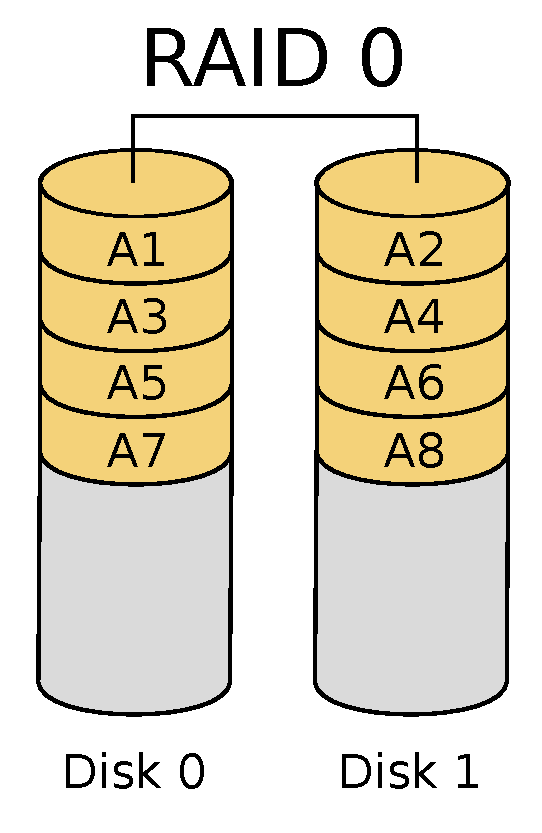
\includegraphics[scale=.4]{RAID_0}

\column{5cm}
将多个磁盘合并成一个大的磁盘,不具有冗余,并行I/O,速度最快。RAID 0亦称为带区集。

%$size = 2 x min(S_1,S_2)$
\end{columns}
\end{frame}

\begin{frame}{RAID1}
\begin{columns}
\column{2cm}
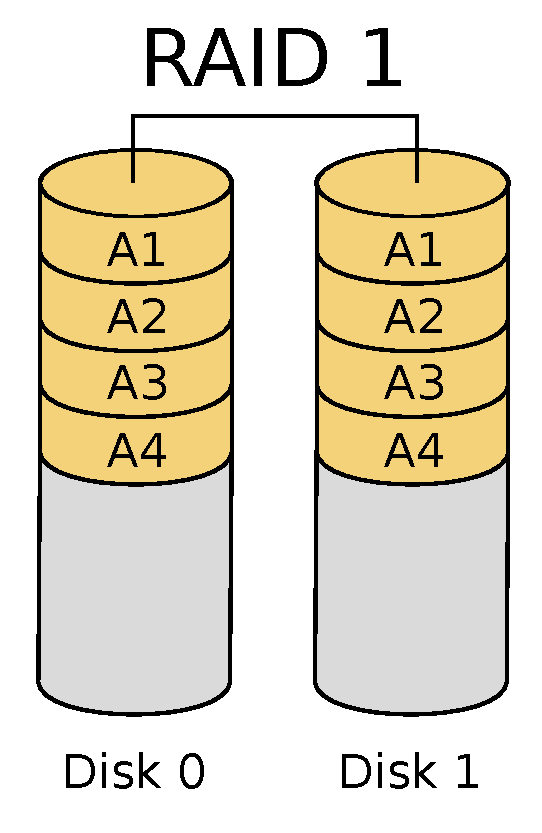
\includegraphics[scale=.4]{RAID_1}

\column{5cm}

两组以上的N个磁盘相互作镜像,在一些多线程操作系统中能有很好的读取速度,另外写入速度有微小的降低。除非拥有相同资料的主磁盘与镜像同时损坏,否则只要一个磁盘正常即可维持运作,可靠性最高。

%$size= min(S_1,S_2)$
\end{columns}
\end{frame}

%\begin{frame}{RAID2}
%\includegraphics{RAID_2}
%
%这是RAID 0的改良版,以汉明码(Hamming Code)的方式将数据进行编码后分割为独立的位元,并将数据分别写入硬盘中。因为在数据中加入了错误修正码(ECC,Error Correction Code),所以数据整体的容量会比原始数据大一些,RAID2最少要三块磁盘方能运作。
%\end{frame}

\begin{frame}{RAID3}

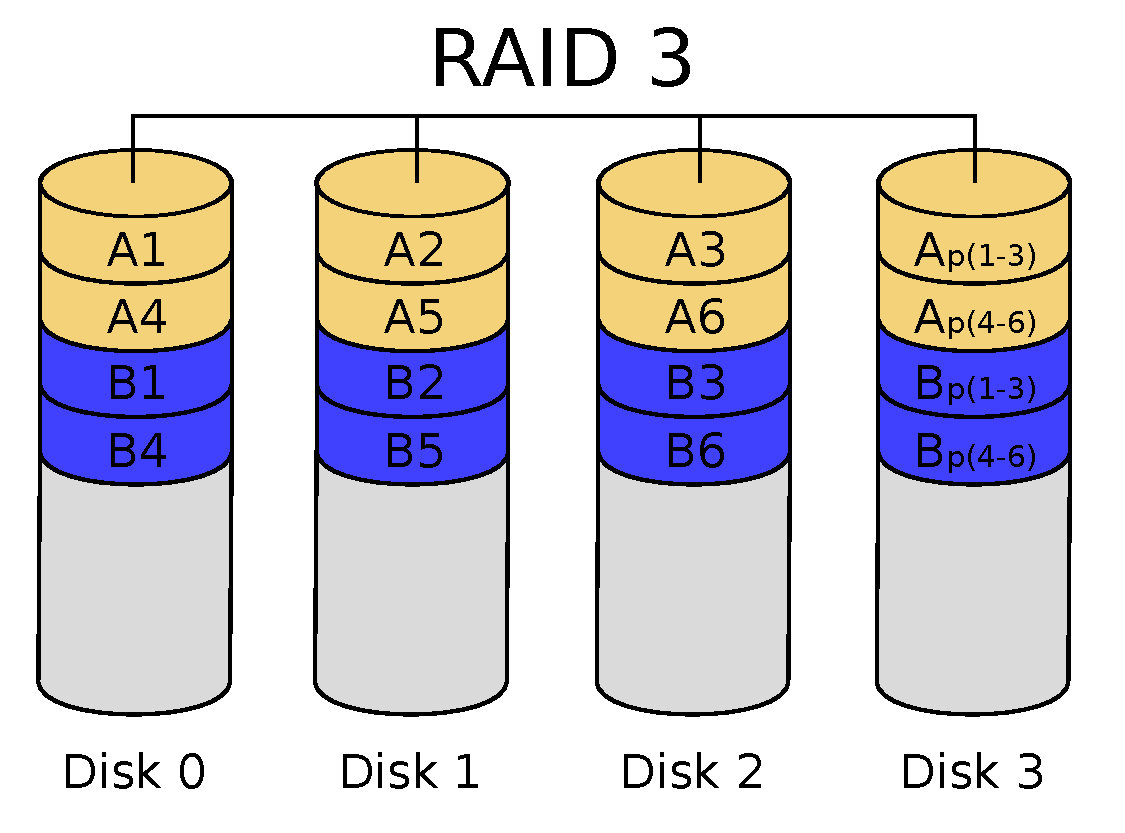
\includegraphics[scale=.4]{RAID_3}

采用Bit-interleaving(数据交错储存)技术,它需要通过编码再将数据位元分割后分别存在硬盘中,而将同位元检查后单独存在一个硬盘中,这种规格比较适于读取大量数据时使用。

\end{frame}

%\begin{frame}{RAID4}
%
%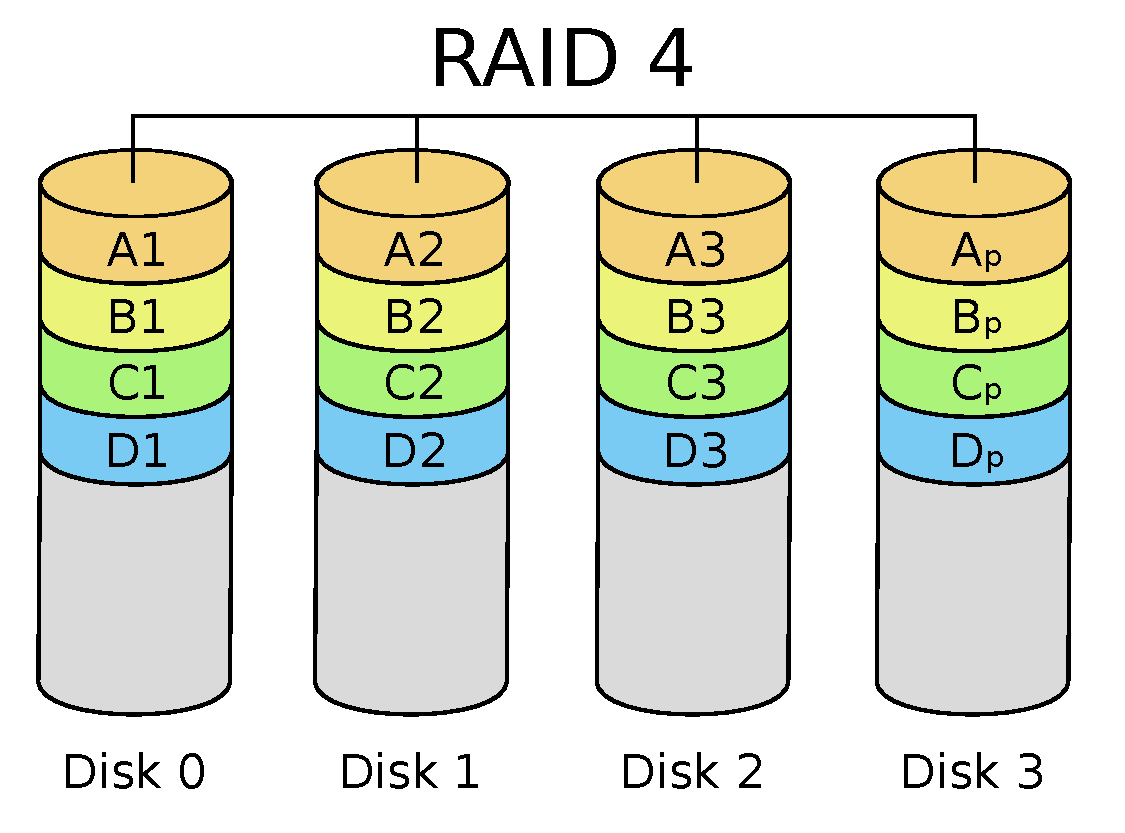
\includegraphics[scale=.4]{RAID_4}
%
%它与RAID 3不同的是它在分割时是以区块为单位分别存在硬盘中,但每次的数据存取都必须从同位元检查的那个硬盘中取出对应的同位元数据进行核对,由于过于频繁的使用,所以对硬盘的损耗可能会提高
%
%
%\end{frame}


\begin{frame}{RAID5}

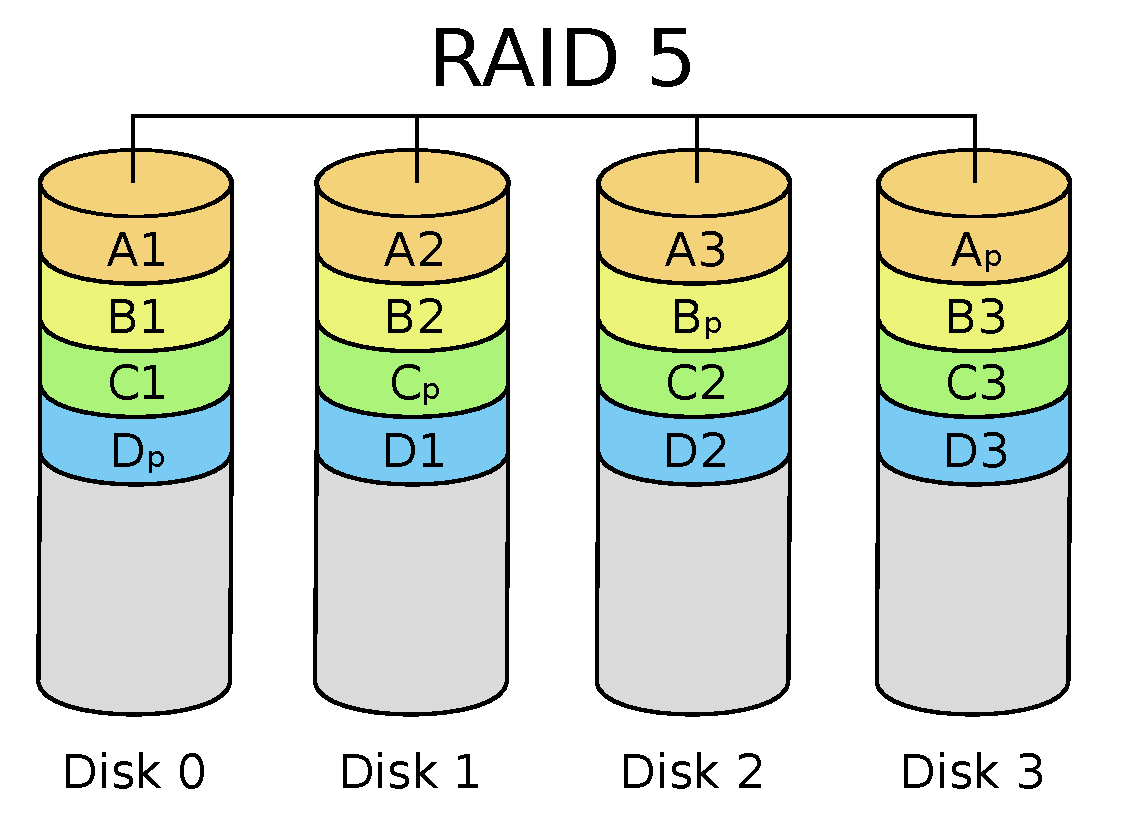
\includegraphics[scale=.4]{RAID_5}


RAID 5 是一种存储性能、数据安全和存储成本兼顾的存储解决方案。它使用的是Disk Striping(硬盘分割)技术。 把数据和相对应的奇偶校验信息存储到组成RAID5的各个磁盘上.并且奇偶校验信息和相对应的数据分别存储于不同的磁盘上。

%$Size = (N -1 ) * min(S_1,S2,\ldots,S_N)$

\end{frame}

\begin{frame}{RAID6}

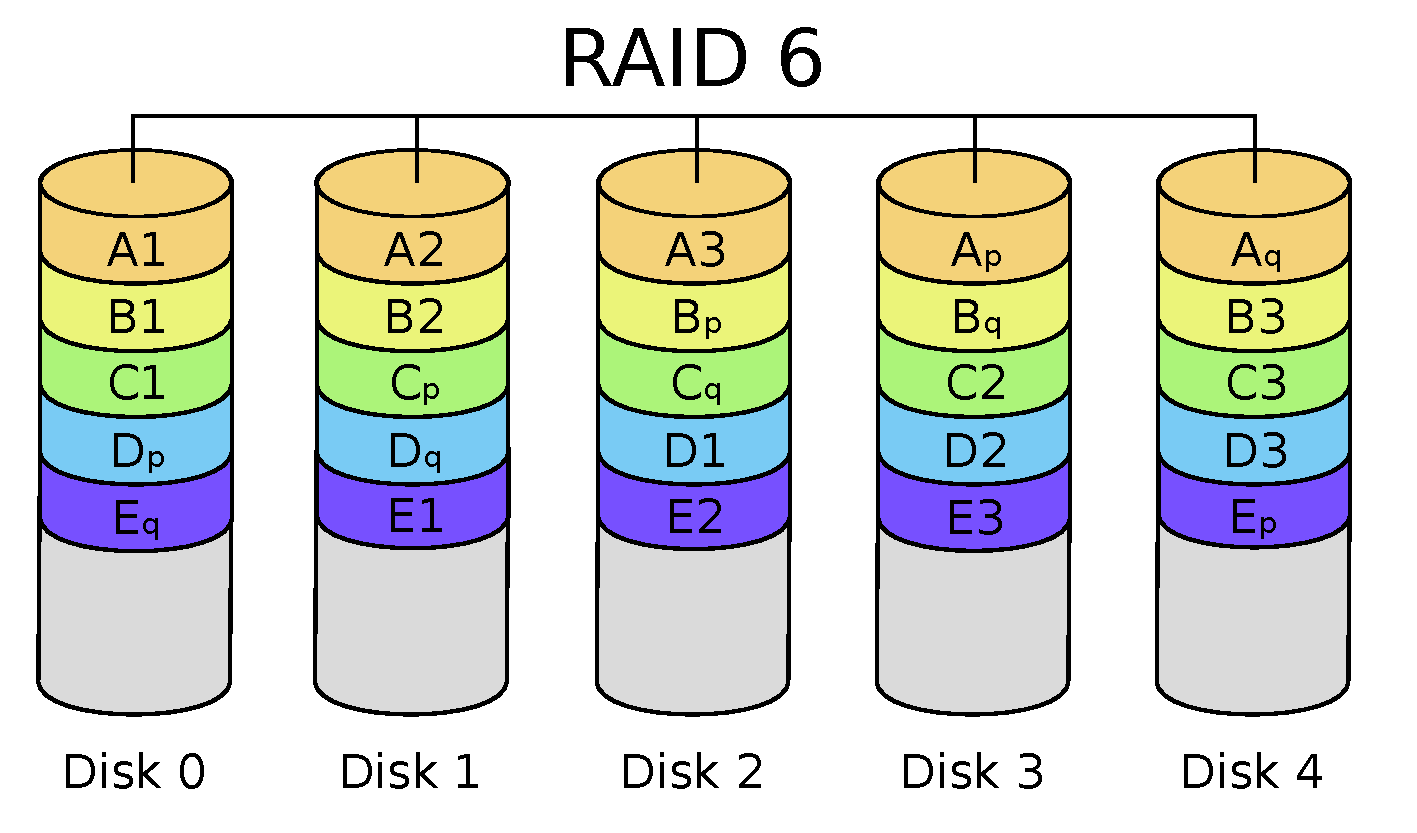
\includegraphics[scale=.4]{RAID_6}


RAID 6相比RAID 5增加了第二个独立的奇偶校验信息块。两个独立的奇偶系统使用不同的算法,数据的可靠性非常高,但相对于RAID 5有更大的“写损失”,因此“写性能”非常差。较差的性能和复杂的实作方式使得RAID 6很少得到实际应用。


\end{frame}

\begin{frame}{RAID10/01}
RAID 1+0是先镜射再分割资料。是将所有硬盘分为两组,视为是RAID 0的最低组合,然后将这两组各自视为RAID 1运作。RAID 1+0有着不错的读取速度,而且拥有比RAID 0更高的资料保护性。 \\
RAID 0+1则是跟RAID 1+0的程序相反,是先分割再将资料镜射到两组硬盘。它将所有的硬盘分为两组,变成RAID 1的最低组合,而将两组硬盘各自视为RAID 0运作。RAID 0+1比起RAID 1+0有着更快的读写速度,不过也多了一些会让整个硬盘组停止运转的机率;因为只要同一组的硬盘全部损毁,RAID 0+1就会停止运作,而RAID 1+0则可以在牺牲RAID 0的优势下正常运作。 \\
至少必须拥有四个以上的偶数硬盘才能使用。
\end{frame}
\subsection{使用软RAID}

\begin{frame}{什么是软RAID}
\begin{itemize}
\item 相比硬件RAID而言,RAID实现由系统完成,而不是RAID卡的固件
\item mdadm 提供了软RAID的管理接口
\item 支持多种RAID级别,包括RAID 0,1,5
\item 支持备用磁盘来增加额外的冗余度
\item RAID设备命名为/dev/md0,/dev/md1,以此类推
\end{itemize}

\end{frame} 

\begin{frame}{软RAID配置}
\begin{itemize}
\item 使用mdadm创建和定义RAID\\
mdadm -C /dev/md0 -a yes -l 1 -n 2 -x 1 /dev/sda1 /dev/sdb1 /dev/sdc1
\item 格式化每一个RAID设备\\
mkfs.ext3 /dev/md0
\item 测试RAID设备
\item mdadm还可以检查RAID设备的状态\\
mdadm --detail /dev/md0
\end{itemize}

\end{frame} 

\begin{frame}{软RAID测试及恢复}
\begin{itemize}
\item 模拟磁盘故障\\
mdadm /dev/md0 -f /dev/sda1
\item 从软RAID磁盘故障中恢复

\begin{itemize}
\item 替换有故障的磁盘
\item 对硬盘进程分区等操作,获得和故障硬盘一样的分区结构
\item mdadm /dev/md0 -a /dev/sda1
\end{itemize}
\item mdadm,/proc/mdstat,/var/log/\{dmesg,messages\}
\item 软RAID遵循RAID规范和限定
\end{itemize}
\end{frame} 
\subsection{使用逻辑卷管理(LVM)}

\begin{frame}{什么是LVM}
\begin{itemize}
\item LVM=Logical Volume Manager
\item 方便处理卷的一个抽象层,包括文件系统的大小更改
\item 允许跨物理设备来组织文件系统

\begin{itemize}
\item 物理设备被当作物理卷 (Physical Volumes, PV)
\item 一个或者多个物理卷组成卷组( Volume Group,VG)
\item 物理卷由固定大小的物理段(Physical Extents,PE)
\item 逻辑卷(Logical Volume,LV)在物理卷上创建,由物理段组成
\item 在逻辑卷上创建文件系统
\end{itemize}
\end{itemize}
\end{frame}

\begin{frame}[plain]{LVM逻辑结构}

\includegraphics[scale=0.5]{lvm.pdf}
\end{frame} 

\begin{frame}{创建逻辑卷(LV)}

\begin{itemize}
\item 创建物理卷\\
pvcreate /dev/hda3
\item 将物理卷分配到卷组\\
vgcreate vg0 /dev/hda3
\item 从特定卷组里创建逻辑卷\\
lvcreate -L 256M -n data vg0\\
mkfs.ext3 /dev/vg0/data 
\item rflvm/system-config-lvm 图形化的配置工具
\end{itemize}

\end{frame} 
\begin{frame}{更改逻辑卷大小}
\begin{itemize}
\item 增大卷

\begin{itemize}
\item lvextend可以增大逻辑卷
\item resize2fs可以在线加大EXT3文件系统
\item vgextend增加新的物理卷到某一个卷组里
\end{itemize}
\item 缩小卷

\begin{itemize}
\item 首先文件系统必须减小
\item 必须\alert{离线}做文件系统检查
\item lvreduce可以减小逻辑卷
\item 卷组可以通过下面的方法减小

\begin{itemize}
\item pvmove /dev/hda3
\item vgreduce vg0 /dev/hda3
\end{itemize}
\end{itemize}
\end{itemize}

\end{frame} 

\begin{frame}{逻辑卷快照}
\begin{itemize}
\item 快照(Snapshot)是一个特殊的逻辑卷,它是在快照生成的时间点对某一个逻辑卷的精确拷贝
\item 采取写时复制技术(Copy on Write, CoW)
\item 快照一般用来执行备份和对某一个数据集的临时拷贝
\item 快照仅仅消耗从快照创建开始,原始卷发生改变需要存储的空间

\begin{itemize}
\item 快照在创建是分配空间,但是并不使用,直到原始卷有改变
\item 当发生改变时,原始卷上老的数据被拷贝到快照上
\end{itemize}
\item \href{http://blog.wgzhao.com/2008/06/20/LVM-snapshot-on.html}{http://blog.wgzhao.com/2008/06/20/LVM-snapshot-on.html}
\end{itemize}
\end{frame}

\begin{frame}[plain]{逻辑卷快照原理图}
\includegraphics[scale=0.6]{lvm-snapshot.pdf}
\end{frame} 

\begin{frame}{使用快照}
\begin{itemize}
\item 对某一个逻辑卷做快照\\
lvcreate -l 30 -s -n backup /dev/vg0/data
\item 挂载快照\\
mkdir -p /mnt/backup\\
mount -o ro /dev/vg0/backup /mnt/backup
\item 删除快照\\
umount /mnt/backup \\
lvremove /dev/vg0/backup
\end{itemize}
\end{frame} 

\subsection{/proc 文件系统}

\begin{frame}{什么是proc文件系统}
在许多类 Unix 计算机系统中, procfs 是 进程 文件系统 (file system) 的缩写,包含一个伪文件系统(启动时动态生成的文件系统),用于通过内核访问进程信息。这个文件系统通常被挂载到 /proc 目录。由于 /proc 不是一个真正的文件系统,它也就不占用存储空间,只是占用有限的内存。
除Linux外,Solaris,BSD,IBM AIX,QNX等均支持proc文件系。
\end{frame}

\begin{frame}{/proc/scsi}
作为系统管理员,需要了解的最有用内容是,在有热插拔硬盘情况下,如何不重启系统就可以添加更多磁盘空间。这里,可以用以下命令来使系统识别新的磁盘:

echo “scsi add-single-device w x y z” > /proc/scsi/scsi

为使该命令正常运行,必须指定正确的参数值 w、x、y 和 z,如下所示:\\
w 是主机适配器(HBA)标识,第一个适配器为零(0) \\
x 是主机适配器上的 SCSI 通道,第一个通道为零(0) \\
y 是设备的 SCSI 标识 \\ 
z 是 LUN 号,第一个 LUN 为零(0) \\


相反的,在不重新引导系统的情况下将设备从系统中除去的命令是:

echo “scsi remove-single-device w x y z” > /proc/scsi/scsi

\end{frame}

\begin{frame}{/proc/sys/fs/}
\begin{exampleblock}{file-max}
该文件指定了可以分配的文件句柄的最大数目。如果用户得到的错误消息声明由于打开文件数已经达到了最大值,从而他们不能打开更多文件,则可能需要增加该值。可将这个值设置成有任意多个文件,并且能通过将一个新数字值写入该文件来更改该值。
\end{exampleblock}

\begin{exampleblock}{file-nr}
该文件与 file-max 相关,它有三个值:
已分配文件句柄的数目
已使用文件句柄的数目
文件句柄的最大数目
该文件是只读的,仅用于显示信息.
\end{exampleblock}

\end{frame}



\begin{frame}{/proc/sys/kernel/}
\begin{description}
\item[hostname] 允许您配置网络主机名。它没有缺省值,也许已经设置了主机名,也许没有设置。
\item[msgmax] 指定了从一个进程发送到另一个进程的消息的最大长度。进程间的消息传递是在内核的内存中进行,不会交换到磁盘上,所以如果增加该值,则将增加操作系统所使用的内存数量。
\item[msgmnb] 指定在一个消息队列中最大的字节数。
\item[msgmni] 指定消息队列标识的最大数目。
\item[panic] 表示如果发生kernel panic 则内核在重新引导之前等待的秒数。0 将禁止重新引导。
\item[shmall] 该文件是在任何给定时刻系统上可以使用的共享内存的总量(以字节为单位)。
\item[shamax] 该文件指定内核所允许的最大共享内存段的大小(以字节为单位)。
\item[shmmni] 该文件表示用于整个系统共享内存段的最大数目
\item[sysrq] 如果该文件指定的值为非零,则激活 System Request Key。
\item[threads-max]  该文件指定内核所能使用的线程的最大数目。
\end{description}
\end{frame}


\begin{frame}{/proc/sys/net/core}
\begin{description}
%\item[message\_burst] 写新的警告消息所需的时间(以 1/10 秒为单位);在这个时间内所接收到的其它警告消息会被丢弃。这用于防止某些企图用消息“淹没”您系统的人所使用的拒绝服务(Denial of Service)攻击。
%\item[message\_cost] 该文件存有与每个警告消息相关的成本值。该值越大,越有可能忽略警告消息。
%\item[netdev\_max\_backlog] 该文件指定了,在接口接收数据包的速率比内核处理这些包的速率快时,允许送到队列的数据包的最大数目。
\item[optmem\_max] 该文件指定了每个套接字所允许的最大缓冲区的大小。

\item[rmem\_default] 该文件指定了接收套接字缓冲区大小的缺省值(以字节为单位)。

\item[rmem\_max] 该文件指定了接收套接字缓冲区大小的最大值(以字节为单位)。

\item[wmem\_default] 该文件指定了发送套接字缓冲区大小的缺省值(以字节为单位)。

\item[wmem\_max] 该文件指定了发送套接字缓冲区大小的最大值(以字节为单位)。
\end{description}
\end{frame}

\begin{frame}{/proc/sys/net/ipv4}
所有 IPv4 和 IPv6 的参数都被记录在内核源代码文档中。请参阅文件 \\ /usr/src/linux/Documentation/networking/ip-sysctl.txt。 \\
或者 \\
/usr/share/doc/kernel-doc-<version>/Documentation/networking/ip-sysctl.txt
\end{frame}

\begin{frame}[allowframebreaks]{/proc/sys/vm}

\begin{exampleblock}{buffermem}
用来控制用于缓存区的内存的大小,它有三个值, \\
第一个用于缓冲区的内存的最低百分比 \\
第二个表示如果发生所剩系统内存不多,而且系统内存正在减少这种情况,系统将试图维护缓冲区内存的数量。 \\
第三个用于缓冲区的内存的最高百分比
\end{exampleblock}


\begin{exampleblock}{freepages}
 该文件控制系统如何应对各种级别的可用内存。它有三个值 \\
第一个表示如果系统中可用页面的数目达到了最低限制,则只允许内核分配一些内存。 \\
第二个表示如果系统中可用页面的数目低于这一限制,则内核将以较积极的方式启动交换,以释放内存,从而维持系统性能。 \\
第三个表示内核将试图保持这个数量的系统内存可用。低于这个值将启动内核交换。
\end{exampleblock}


\begin{exampleblock}{kswapd}
该文件控制允许内核如何交换内存。它有三个值\\
第一个表示内核试图一次释放的最大页面数目。如果想增加内存交换过程中的带宽,则需要增加该值。\\
第二个表示内核在每次交换中试图释放页面的最少次数。\\
第三个内核在一次交换中所写页面的数目。这对系统性能影响最大。这个值越大,交换的数据越多,花在磁盘寻道上的时间越少。然而,这个值太大会因“淹没”请求队列而反过来影响系统性能。
\end{exampleblock}
\end{frame}

\begin{frame}{修改proc值}
\begin{itemize}
\item echo 重定向,即时生效,重启生效  \\
	echo 1 >/proc/sys/net/ipv4/icmp\_echo\_ignore\_all
\item sysctl 修改/proc/sys下的值,即时生效,重启失效   \\
	sysctl -w net.ipv4.icmp\_echo\_ignore\_all
\item 修改/etc/sysctl.conf,重启后依然有效
\end{itemize}
\end{frame}


\subsection{文件归档}

\begin{frame}{归档工具:tar}
\begin{itemize}
\item tar 可以备份到一个文件或者磁带设备上
\item 支持gzip和bzip2压缩
\item 能保留文件许可,拥有关系和时间戳
\item 支持扩展属性
\item 使用 rmt 指令可以写入到远程磁带设备
\end{itemize}

\end{frame} 
\begin{frame}{归档工具:dump/restore}
\begin{itemize}
\item 备份和恢复ext2/ext3文件系统

\begin{itemize}
\item 其他文件系统目前不支持
\item dump应该仅对没有挂载的或者只读的文件系统操作
\end{itemize}
\item 能做完全或者增量备份
\item 例子\\
dump -0u -f /dev/st0 /dev/hda2\\
restore -rf /dev/st0
\end{itemize}

\end{frame} 
\begin{frame}{归档工具:rsync}
\begin{itemize}
\item 高效的文件拷贝,无论是从远程,还是到远程
\item 使用ssh连接来做安全数据传输\\
rysnc {*}.dbf xplore:/data/backup
\item 比scp更快---差异性拷贝
\end{itemize}
\end{frame} 
%\subsection{实验}
%
%\begin{frame}{实验I:配置实现配额}
%
%
%
%要求:用户victor在/home下使用空间不能超过1024K
%
%提示:
%\begin{enumerate}
%\item 创建用户victor
%\item 对/home激活配额
%\item 设置配额值包括soft和hard
%\item 测试
%\end{enumerate}
%
%\end{frame} 
%\begin{frame}{实验II:软RAID实践}
%\begin{description}
%\item [{场景:}] 一个关键应用需要安装在冗余介质上。于是做出了在现有系统上使用软RAID的决定。修改你的系统配置使得支持带热备的镜像阵列
%\item [{要求:}] 带自动失效恢复(auto-fail-over)的RAID 1 系统
%\end{description}
%提示
%\begin{enumerate}
%\item 创建需要的分区或者设备
%\item 使用mdadm
%\item 测试
%\end{enumerate}
%
%\end{frame} 
%\begin{frame}{实验II:逻辑卷操作}
%\begin{description}
%\item [{场景:}]~\end{description}
%\begin{enumerate}
%\item 为了让新创建的RAID能够共享给多个应用,决定在RAID设备上部署LVM。一个逻辑卷需要创建为ext3文件系统。
%\item 需要增加一个卷组来为总是要求额外空间的应用提供服务。创建这个卷组,使其包含两个分区,新的分区能够加入进来,新的文件系统可以扩展
%\item 老的应用程序数据不再增加,通过备份,调整后,需要的空间相比最初少了很多,为了节省空间,需要把空闲的空间分离出来。\end{enumerate}
%\begin{description}
%\item [{要求:}] 创建LVM,并根据需要扩展,缩小逻辑卷大小
%\end{description}
%\end{frame} 
%
%\section{性能调优}
%
%
%\section{虚拟化}
%
%
%\subsection{概述}
%
%
%
%\begin{frame}{虚拟化}
%
%目标
%\begin{itemize}
%\item 什么是虚拟化
%\item 理解Xen技术
%\item 理解KVM技术
%\item 虚拟化工具链
%\item Xen 工具
%\item KVM 工具
%\end{itemize}
%
%\end{frame} 
%\begin{frame}{优势}
%\begin{itemize}
%\item 资源的高效使用
%\item 可管理性
%\item 安全性
%\item 更低的总拥有成本(CTO)
%\end{itemize}
%\end{frame} 
%\subsection{Xen的虚拟化}
%
%
%
%\begin{frame}{Xen的关键概念}
%\begin{itemize}
%\item 超级监控器(Hypervisor)小巧
%\item 第一个域('Domain')管理系统
%\item 支持完全虚拟化和半虚拟化
%\end{itemize}
%
%\end{frame} 
%\begin{frame}{硬件的考虑因素}
%\begin{itemize}
%\item 最低要求
%
%\begin{itemize}
%\item 带PAE支持的CPU
%\item 每一个 Domain 256MB 内存
%\item 每个 Domain 6GB 磁盘空间
%\end{itemize}
%\item 额外的考虑因素
%
%\begin{itemize}
%\item 对于完全虚拟化,需要带VT/SVM功能的CPU支持
%\item 在线迁移的实现有赖于共享存储
%\item 应用程序的不同导致需要的存储空间大小也不同
%\end{itemize}
%\end{itemize}
%
%\end{frame} 
%\begin{frame}{准备Domain-0}
%\begin{itemize}
%\item 安装Domain0(大部分发行版本自带)
%\item 启动Xen Hypervisor
%\item 启动xend 管理守护进程
%\end{itemize}
%
%\end{frame} 
%\begin{frame}{虚拟资源}
%\begin{itemize}
%\item CPU
%
%\begin{itemize}
%\item 使用VCPU (Virtual CPUs)
%\item 不需要直接映射到真实CPU上
%\end{itemize}
%\item 存储
%
%\begin{itemize}
%\item 块设备
%\item 简单文件
%\end{itemize}
%\item 网络设备
%
%\begin{itemize}
%\item 网桥或者到Domain0的路由
%\item 默认是映射到xenbr0设备上
%\end{itemize}
%\end{itemize}
%
%\end{frame} 
%\begin{frame}{Domain-U 配置}
%\begin{itemize}
%\item 定义每一个Domain-U
%\item 虚拟块设备
%\item CPUs
%\item 网络
%\item /etc/xen/\emph{domain}
%\end{itemize}
%
%\end{frame} 
%\begin{frame}{安装新的Domain-U}
%\begin{itemize}
%\item 虚拟管理器(virt-manager)
%
%\begin{itemize}
%\item 管理 domain 的图形前端
%\item 提供了设置一个新 domain 的向导
%\item 是 xm 命令行工具的有效替代方案
%\end{itemize}
%\item 定义 domain 的名字
%\item 选择存储类型和 CPU 个数
%\item 指定安装程序的位置或者kickstart文件的位置(可选)
%\end{itemize}
%
%\end{frame} 
%\begin{frame}{用 xm 管理 domain}
%\begin{itemize}
%\item 命令行管理工具
%\item 控制 domain
%
%\begin{itemize}
%\item xm < create | destroy>
%\item xm <pause | unpause>
%\item xm <save | restore> \emph{filename}
%\item xm <shutdown | reboot>
%\end{itemize}
%\item 监控
%
%\begin{itemize}
%\item xm list
%\item xentop
%\item xen console
%\end{itemize}
%\end{itemize}
%
%\end{frame} 
%\begin{frame}{启动时激活 Domain}
%\begin{itemize}
%\item xendomains 脚本
%\item xendomains <start | stop>
%\item 必须链接 domain 配置文件到 /etc/xen/auto
%\end{itemize}
%\end{frame} 
%\subsection{KVM的虚拟化}





%%\part{网络服务}

%\begin{frame}{网络服务}
%	\tableofcontents[currentsection]
%\end{frame}

\section{服务访问控制}

\begin{frame}{服务访问控制}

目标
\begin{itemize}
\item 理解服务是如何管理的
\item 了解服务的共同特性
\item 描述服务配置资源
\item 访问控制实现
\end{itemize}

\end{frame} 
\begin{frame}{init管理的系统资源}
\begin{itemize}
\item 服务监听在串口协议连接上

\begin{itemize}
\item 串口终端
\item 调制解调器(modem)
\end{itemize}
\item 配置文件 /etc/inittab
\item 调用命令rc来执行初始化脚本
\item 调用脚本开始X11 显示管理器
\item 提供respawn能力

\begin{itemize}
\item 1:2345:respawn:/sbin/mingetty tty1
\end{itemize}
\end{itemize}

\end{frame} 
\begin{frame}{服务管理}
\begin{itemize}
\item 一般指的是'System V' 或'SysV'

\begin{itemize}
\item 脚本层级结构由文件系统目录来组织
\item 服务可以激活也可以禁止
\end{itemize}
\item 通常都有服务配置文件
\item 大部分服务启动一个或多个进程
\item 命令由脚本“包裹”(wrap)
\item 服务由/etc/init.d/目录下的脚本管理
\item 举例

\begin{itemize}
\item /etc/init.d/network status
\item service network status
\end{itemize}
\end{itemize}

\end{frame} 
\begin{frame}{chkconfig}
\begin{itemize}
\item 管理服务在各运行级别上的限定
\item 希望启动时运行网络服务:\\
chkconfig network on
\item 并不修改当前服务的运行状态
\item 用于独立的服务
\item 可以被其他应用程序调用,包括rfsysv
\item 列出运行级别服务状态表,执行\\
chkconfig --list
\end{itemize}

\end{frame} 
\subsection{xinetd 服务}


\begin{frame}{xinetd管理的服务}
\begin{itemize}
\item 管理按需启动的服务,且使用较少或者使用时间短暂

\begin{itemize}
\item 需求不太频繁的服务
\item 基于主机的认证
\item 服务统计和日志记录
\item 服务IP重定向
\end{itemize}
\item 配置文件 /etc/xinetd.conf,/etc/xinetd.d/\emph{service}
\item 与libwrap.so 连接
\item 服务可以由chkconfig 控制\\
chkconfig telnet on
\end{itemize}

\end{frame} \begin{frame}{xinetd 缺省控制}

顶级配置文件--xinetd.conf

\verbatiminput*{/etc/xinetd.conf}


\end{frame} \begin{frame}{xinetd服务配置}

服务配置文件 /etc/xinetd.d/\emph{service}

/etc/xinetd.d/telnet

service telnet

\{

disable = yes

flags = REUSE

socket\_type = stream 

wait = no

user = root

server = /usr/sbin/in.telnetd

log\_on\_failure += USERID

\}


\end{frame} 
\begin{frame}{xinetd访问控制}
\begin{itemize}
\item 可以写在/etc/xinetd.conf中,也可以写在/etc/xinetd.d/目录下的文件中
\item 也可以使用的控制语句

\begin{itemize}
\item 允许 only\_from = \emph{客户端描述}
\item 拒绝 no\_access = \emph{客户端描述}
\item per\_source = \emph{数量}
\item access\_time = \emph{客户端描述}
\end{itemize}
\end{itemize}

\end{frame} 
\begin{frame}{/etc/sysconfig/ 文件}
\begin{itemize}
\item 某些服务需要该目录下的配置文件来确定服务如何运行

\begin{itemize}
\item named
\item sendmail
\item dhcpd
\item samba
\item init
\item syslog
\end{itemize}
\end{itemize}

\end{frame} 
\begin{frame}{服务和应用访问控制}
\begin{itemize}
\item 特定服务配置

\begin{itemize}
\item 像httpd,smbd,squid等守护进程,都提供了自身的安全机制
\end{itemize}
\item 通用配置

\begin{itemize}
\item 所有程序都和libwrap.so关联,使用通用的配置文件
\item 因为xinetd和libwrap.so关联,因此影响到它提供的服务
\item 检查主机和远程用户名
\end{itemize}
\end{itemize}

\end{frame} 
\subsection{网络实验}


\begin{frame}{实验I:浏览Xinetd服务}
\begin{description}
\item [{场景:}] 系统安装了telenet软件包,希望被xinetd超级守护进程管理。telnet服务在需要的时候变得有效,当没有用户连接时,系统中并不存在telnet进程
\item [{要求:}] 配置基于xinetd管理的telnet服务
\end{description}

\end{frame} 
\section{远程访问服务器}

\begin{frame}{运程访问服务器}

目标
\begin{itemize}
\item 理解openssh的安全特性
\item 通过openssh远程访问于数据传输
\item 理解远程图形化访问
\item 掌握VNC使用
\end{itemize}

\end{frame} 
\subsection{OpenSSH 概述}



\begin{frame}{OpenSSH 概述}
\begin{itemize}
\item OpenSSH替代之前常用的非安全网络通信程序
\item 提供用户和基于令牌的认证
\item 提供通过端口转发将非安全协议建立在隧道(tunnel)内的能力
\item 系统缺省配置(客户端,服务端)位于/etc/ssh
\end{itemize}

\end{frame} 
\begin{frame}{OpenSSH 认证}
\begin{itemize}
\item sshd守护进程能够利用几个不同的认证方法

\begin{itemize}
\item 密码(安全发送)
\item RSA/DSA 键
\item Kerberos
\item s/key和安全ID
\item 使用系统键值的主机认证
\end{itemize}
\end{itemize}

\end{frame} 
\begin{frame}{OpenSSH 服务器}
\begin{itemize}
\item 在网络系统里提供极大的数据安全

\begin{itemize}
\item 公/私钥 加密
\item 和早期的SSH行业版本兼容
\end{itemize}
\item 通过libwrap.so实现基于主机的安全
\end{itemize}

\end{frame} 
\begin{frame}{OpenSSH 服务一览}
\begin{itemize}
\item 类型:SysV管理的服务
\item 软件包:openssh,openssh-clients,openssh-server
\item 守护进程:/usr/sbin/sshd
\item 脚本:/etc/init.d/sshd
\item 端口:22(可配置)
\item 配置:/etc/ssh/{*},\$HOME/.ssh/
\item 相关:openssl,openssh-askpass,tcp\_wrappers
\end{itemize}

\end{frame} 
\subsection{OpenSSH 配置}



\begin{frame}{OpenSSH 服务配置}
\begin{itemize}
\item sshd 配置文件: /etc/ssh/sshd\_config
\item 可考虑的配置选项

\begin{itemize}
\item Protocol
\item ListenAddress
\item PermitRootLogin
\item Banner
\end{itemize}
\end{itemize}

\end{frame} 
\begin{frame}{OpenSSH 客户端}
\begin{itemize}
\item 安全shell会话

\begin{itemize}
\item ssh \emph{hostname}
\item ssh \emph{user@hostname}
\item ssh \emph{hostname remote-command}
\end{itemize}
\item 远程文件和目录安全拷贝

\begin{itemize}
\item scp\emph{ file user@host:remote-dir}
\item scp -r \emph{user@host:remote-dir localdir}
\end{itemize}
\item sshd提供的安全ftp

\begin{itemize}
\item sftp \emph{host}
\item sftp -C \emph{user@host}
\end{itemize}
\end{itemize}

\end{frame} 
\begin{frame}{应用:RPM}
\begin{itemize}
\item 文件一致性的两种实现
\item 已经安装的文件

\begin{itemize}
\item MD5 单向哈希(hash)
\item rpm --verify/-V \emph{package\_name}
\end{itemize}
\item 发行包文件

\begin{itemize}
\item GPG公钥签名
\item rpm --import /etc/pki/rpm-gpg/RPM-GPG-KEY-redflag{*}
\item rpm --checksig/-K \emph{package\_file\_name}
\end{itemize}
\end{itemize}

\end{frame} 
\subsection{VNC:虚拟网络计算}


\begin{frame}{VNC:Virutal Network Computing}
\begin{itemize}
\item 允许通过网络访问或者共享完整的桌面环境

\begin{itemize}
\item 作为纯粹的X链接占用带宽极少
\item 服务端

\begin{itemize}
\item 每个独立用户都可以启动vncserver命令启动vnc服务
\item 运行\$HOME/.vnc/xstartup运行vnc服务
\item 可以设定不同于系统帐号密码的密码
\item 通过/etc/init.d/vncserver可以自启动vnc服务
\end{itemize}
\item 客户端

\begin{itemize}
\item 使用vncviewer host:screen 连接远程机器
\item 同一主机通过唯一的屏幕号来区分
\item 支持通过ssh隧道来链接 vncviewer -via user@remote localhost:1
\end{itemize}
\end{itemize}
\end{itemize}

\end{frame} 
\section{网络域名服务}

\begin{frame}{网络域名服务(DNS)}

目标
\begin{itemize}
\item 理解主机名解析和在网络系统组织上的作用
\item 使用普通程序探索和校验DNS服务操作
\item 描述域名系统(Domain Name System,DNS)
\item 配置基本的DNS服务
\end{itemize}

\end{frame} 
\subsection{DNS 原理}


\begin{frame}{DNS 概述}
\begin{itemize}
\item 把主机名解析成IP地址(正向查找)
\item 把IP地址解析成主机名(反向查找)
\item 允许多台机器成为一个逻辑组

\begin{itemize}
\item hostname.doman.tld
\item hostname.subdomain.domain.tld
\end{itemize}
\item 每一个名字服务器响应名字空间的一部分,成为区(zone)
\item 名字服务起缓存应答
\end{itemize}



\end{frame} 
\begin{frame}{DNS特定的解析器}
\begin{itemize}
\item host

\begin{itemize}
\item 永远不读/etc/nsswitch.conf
\item 缺省情况下,查找/etc/resolv.conf文件里的nameserver和search行
\item 缺省是最小化输出
\end{itemize}
\item dig

\begin{itemize}
\item 永远不读/etc/nsswitch.conf
\item 缺省情况下,仅查找/etc/resolv.conf文件里的nameserver 行
\item 输出是RFC标准的zone文件格式,该格式用于DNS服务
\end{itemize}
\end{itemize}

\end{frame} 
\begin{frame}{dig跟踪DNS查询}
\begin{itemize}
\item dig + trace redflag-linux.com

\begin{itemize}
\item 读取 /etc/resolv.conf 来决定名字服务器
\item 查询根名字服务器
\item 逐级查询名字记录
\end{itemize}
\item 上述被称为迭代查询(iterative query)
\item 初步观察:

\begin{itemize}
\item 名字组织成倒立数结构,根(.)在顶端
\item 名字层次结构允许DNS跨组织边界
\item 全质量主机名(QFDN)以点(.)结尾
\end{itemize}
\end{itemize}

\end{frame} 
\begin{frame}{其他观察}
\begin{itemize}
\item 每一条应答记录是以资源记录(resource record)形式展现的
\item 每一个资源记录有5个域

\begin{description}
\item [{domain}] 查询的域或者子域
\item [{ttl}] 记录缓存的秒数
\item [{class}] 记录分类(通常是IN)
\item [{type}] 记录类型,比如A,NS
\item [{rdata}] domain映射的资源数据
\end{description}
\item 概念上讲,对一个域的查询,映射到rdata就是一个应答
\end{itemize}

\end{frame} 
\begin{frame}{邮件交换Mail Exchanger)查询}
\begin{itemize}
\item 一条MX记录映射域名到一台邮件服务器的完全合格域名(full-qualified domain name,FQDN)上
\item dig -t mx redflag-linux.com
\item 观察

\begin{itemize}
\item rdata 域被扩充,加入了一块额外的数据,称为优先级(priority)
\item 优先级可以看作是网络的距离,网络偏爱短路径
\item 为了避免额外的查询,域名服务器通常在MX记录里提供一个额外的和FQDN响应的A记录
\item MX记录以及和它关联的A记录组成了域的邮件服务
\end{itemize}
\end{itemize}

\end{frame} 
\begin{frame}{zone,domain,authoritative}
\begin{itemize}
\item 一个域(domain)包含一个完整的分级域名下层树
\item 一个区(zone)则是域的一部分,被一个具体详细的服务器所管理
\item 子域可以被授权成为附加的域
\item 一个区可以直接管理子域
\end{itemize}

\end{frame} 
\begin{frame}{host 探测DNS}
\begin{itemize}
\item 下面的命令,增加-v参数可以看到以zone文件格式输出
\item 跟踪:无效
\item 委派:host -rt ns google.com
\item 强制迭代:host -r google.com
\item 反向查询:host 74.125.53.100
\item MX 查询:host -t mx redflag-linux.com
\item SOA 查询:host -t soa redflag-linux.com
\item 区传送:host -t axfr redflag-linux.com 192.168.1.2 or\\
host -t ixfr=\emph{serial} redflag-linux.com. 192.168.1.2
\end{itemize}

\end{frame} 
\subsection{BIND 概述}


\begin{frame}{Berkely Internet Name Domain}
\begin{itemize}
\item 一般称为BIND,运行为 named
\item BIND是互联网上应用最广泛的DNS服务器

\begin{itemize}
\item 提供正向查询,反向查询,转发和缓存功能
\item DNS RFC规范的参考实现
\item 运行在chroot环境下
\item 能同时为不同的域充当主(master)服务器和辅助(slave)服务器
\end{itemize}
\end{itemize}

\end{frame} 
\begin{frame}{BIND服务一览}
\begin{itemize}
\item 类型:SysV 管理的服务
\item 包:bind,bind-utils,bind-chroot
\item 守护进程:/usr/sbin/named,/usr/sbin/rndc
\item 脚本:/etc/init.d/named
\item 端口:53(域),953(rndc)
\item 配置:{[}/var/named/chroot{]}/etc/named.conf,/var/named/{*},/etc/rndc.key
\item 相关包:caching-nameserver,openssl
\item /etc/sysconfig/named
\item named 进程被SysV脚本激活后,会根据此文件的参数决定运行参数
\end{itemize}

\end{frame} 
\begin{frame}{开始BIND}
\begin{itemize}
\item 安装相关软件包

\begin{itemize}
\item bind 核心二进制程序
\item bind-chroot 安全考虑
\item caching-nameserver 初始配置
\end{itemize}
\item 开始配置

\begin{itemize}
\item service named configtest
\item service named start
\item chkconfig named on
\end{itemize}
\item 处理基本的named配置
\end{itemize}

\end{frame} 
\subsection{BIND 配置}


\begin{frame}{/etc/named.conf}
\begin{itemize}
\item named.conf 是BIND使用的默认配置文件
\item 在每一次named启动与挂起时都会被读取
\item 一个简单的文本文件,其中记录的可以包括options(全局参数)、zone(区域定义)、access control lists (访问控制列表)等
\end{itemize}

\end{frame} 
\begin{frame}{option}
\begin{itemize}
\item 在/etc/named.conf的options段申明
\item 常用的参数包括

\begin{description}
\item [{directory}] 指定zone文件的存放位置
\item [{forwarders}] 指定其商机域名服务器
\item [{allow-query}] 指定允许向其提交请求的客户
\item [{allow-transfer}] 指定允许复制zone数据的主机
\end{description}
\end{itemize}

\end{frame} 
\begin{frame}{主域}


\begin{itemize}
\item 由一个zone段在/etc/named.conf中申明
\item type master;
\item file:存放该zone数据的文件名

\begin{itemize}
\item 必须存在于options段中提及的目录之下
\item 文件名可以随意
\end{itemize}
\item allow-update:允许动态更新该zone数据的客户机
\end{itemize}

\end{frame} 
\begin{frame}{从域}
\begin{itemize}
\item 由一个zone段在/etc/named.conf中申明
\item type slave;
\item master:指定其主域名服务器

\begin{itemize}
\item 对应的主域名服务器必须承认并存放有该区域的数据
\end{itemize}
\item file:本地用于存放zone数据的文件
\item 从域名服务器总是试图与其master联系并获取一份当前数据的副本
\end{itemize}

\end{frame} 
\begin{frame}{反向解析域}


\begin{itemize}
\item 域的名字必须用.in-addr.arpa来结尾
\item 由一个zone段在/etc/named.conf中宣告
\item 反解析域一般对应到一个具体的IP段
\item 反解析域同样可以配置为从域
\item 许多服务会尝试进行反解析
\end{itemize}



\end{frame} 
\begin{frame}{zone文件}
\begin{itemize}
\item 文件通常存放在/var/named目录下
\item 以\$TTL开头
\item ; 后面表示注释
\item 包含的资源记录

\begin{itemize}
\item A 名字到IP地址的映射
\item PTR IP地址到名字的映射
\item CNAME 创建别名
\item MX 邮件交换记录
\end{itemize}
\item FQDN必须以.结尾
\item 每一个在/etc/named.conf中定义的zone都应该对应一个具体的zone文件
\end{itemize}

\end{frame} 
\begin{frame}{(resource record)资源记录}
\begin{description}
\item [{SOA}] 定义起始授权
\item [{NS}] 指定域名服务器
\item [{MX}] 指定邮件服务器
\item [{A}] 将一个域名解析成其后的IP
\item [{CNAME}] 将一个域名设置为另一个域名的别名
\item [{PTR}] 将一个IP地址指向一个域名/主机名
\end{description}

\end{frame} 
\begin{frame}{SOA 记录}


\begin{itemize}
\item SOA(Start of Authroity):起始授权
\item 在每一个域文件中都应该有一个SOA段\\
@       IN      SOA     localhost. root.localhost.  (
\end{itemize}
                                      1997022700 ; Serial

                                      28800      ; Refresh

                                     14400      ; Retry

                                      3600000    ; Expire

                                      86400 )    ; Minimum


\end{frame} 
\begin{frame}{NS 记录}


\begin{itemize}
\item NS(name server):域名服务器
\item 每一个主域名服务器和从域名服务器都应该拥有一条NS记录,以防止主服务器在出现故障后,从服务器不能及时提供服务\\
@			IN    	NS	server1.example.com.\\
example.com	IN	NS	server1.example.com.
\end{itemize}

\end{frame} 
\begin{frame}{Round Robin}
\begin{itemize}
\item 利用复数A记录来均衡数台服务器的访问负载 \\
www 0 IN A 192.168.0.3\\
www 0 IN A 192.168.0.4\\
www 0 IN A 192.168.0.5
\item round robin的关键在于,每一条A记录都不应该被记入cache。 
\end{itemize}

\end{frame} 
\begin{frame}{Remote Name Daemon Control(rndc)}
\begin{itemize}
\item 提供本地和远程named 管理
\item bind-chroot 包配置rndc

\begin{itemize}
\item 仅监听在本地回路上
\item 从/etc/rndc.key读取key
\item 如果key不匹配,则不能启动或者停止named 服务
\item 本地安装,缺省下,不需要额外的配置
\end{itemize}
\item 例如: rndc flush 清空服务器缓存
\end{itemize}

\end{frame} 
\begin{frame}{BIND 语法检查工具}


\begin{itemize}
\item named-checkconf -t \emph{ROOTDIR /path/to/named.conf}

\begin{itemize}
\item 缺省检查/etc/named.conf(如果没有指定-t参数)
\item named-checkconf -t /var/named/chroot
\end{itemize}
\item named-checkzone \emph{origin /path/to/zonefile}

\begin{itemize}
\item 检查指定的zone配置文件
\item 举例:\\
named-checkzone xplore.cn /var/named/chroot/var/named/xplore.cn.zone
\end{itemize}
\end{itemize}

\end{frame} 
\begin{frame}{rfdns}
\begin{itemize}
\item 图形界面下的BIND配置工具
\item 简单清晰的完成BIND配置
\item 每一个配置都有对应的配置文件的更新试图,非常适合对BIND的配置学习
\item 可对应多个版本的BIND
\end{itemize}

\end{frame} 
\begin{frame}{bind-chroot 软件包}
\begin{itemize}
\item 在/var/named/chroot下安装chroot环境
\item 把已有的配置文件移到chroot环境,用符号链接替换原始文件
\item 更新/etc/sysconfig/named文件,加入或者修改:\\
ROOTDIR=/var/named/chroot
\item Tips

\begin{itemize}
\item 安装bind-chroot后,检查/etc/sysconfig/named文件
\item 启动named后执行ps -ef |grep named校验启动选项
\end{itemize}
\end{itemize}

\end{frame} 
\begin{frame}{caching-nameserver 软件包}
\begin{itemize}
\item 提供:

\begin{itemize}
\item named.caching-nameserver.conf
\item named.ca 包含根服务'hints'
\item 本地机器名和IP地址的的正向和反向查询zone文件(localhost.localdomain)
\end{itemize}
\item Tips

\begin{itemize}
\item 拷贝named.caching-nameserver.conf 为named.conf
\item 改变文件所有权关系:chown root:named
\item 编辑named.conf
\end{itemize}
\end{itemize}

\end{frame} 
\subsection{DNS实验}


\begin{frame}{[shrink=5]实验I:用BIND工作}


\begin{description}
\item [{场景:}] 为了加快网络交易和降低出口带宽占用,你的机构确定部署cacheing name server,激活服务器。分别需要解析下面的主机名\\
\begin{tabular}{|c|c|c|}
\hline 
IP地址 & 主机名 & 别名\tabularnewline
\hline 
\hline 
192.168.2.2 & hr.domain.com & -\tabularnewline
\hline 
192.168.2.3 & sales.domain.com & -\tabularnewline
\hline 
192.168.2.4 & tech.domain.com & support\tabularnewline
\hline 
192.168.2.5 & mail.domain.com & smtp,pop3\tabularnewline
\hline 
\end{tabular}\\
其中mail.domain.com作为该域的邮件服务器,所有主机需要能正向查询和反向查询
\item [{要求:}] 配置caching name server,从安装角度考虑,使用chroot环境。
\end{description}





\end{frame} 
\section{DHCP服务}



\begin{frame}{DHCP 服务}
\begin{itemize}
\item DHCP : Dynamic Host Configuration Protocol,通过dhcpd 实现
\item dhcpd 可以同时为DHCP和BOOTP客户端提供服务
\end{itemize}

\end{frame} 
\begin{frame}{DHCP 服务一览}
\begin{itemize}
\item 类型:SysV管理的服务
\item 软件包:dhcp
\item 守护进程:/usr/sbin/dhcpd
\item 脚本:/etc/init.d/dhcpd
\item 端口:67(bootps),68(bootpc)
\item 配置文件:/etc/dhcpd.conf,/var/lib/dhcpd/dhcpd.leases
\end{itemize}

\end{frame} 
\begin{frame}{配置DHCP服务}
\begin{itemize}
\item /etc/dhcpd.conf
\item /usr/share/doc/dhcp-\emph{version}/dhcpd.conf.sample
\item 必须至少有一个子网块,必须和配置的网络接口对应
\item service dhcpd configtest 检查语法
\item rfdhcp 图形化配置工具
\end{itemize}

\end{frame} 
\begin{frame}{DHCP服务配置举例}

subnet 192.168.0.0 netmask 255.255.255.0 \{

	range 192.168.0.2 192.168.0.253;

	default-lease-time 21600;

	max-lease-time 43200;

	option domain-name “example.com”;

	option routers 192.168.0.254;

	option domain-name-servers  192.168.0.254;

\}




\end{frame} 
\begin{frame}{常用DHCP配置参数}
\begin{itemize}
\item subnet x.x.x.x netmask x.x.x.x 指定dhcp服务工作网段
\item range 指定分配地址段
\item default-lease-time 默认租赁期
\item max-lease-time 最大租赁期
\item option routers 分配路由器
\item option domain-name 分配域名
\item option domain-name-servers 分配DNS服务器
\end{itemize}

\end{frame} 
\begin{frame}{IP 绑定}
\begin{itemize}
\item host \emph{name}为绑定主机起名(不是分配给对方的主机名)
\item hardware ethernet \emph{mac-addr }指定硬件地址
\item fixed-address \emph{ipaddr} 指定ip地址或者主机名
\item 支持为绑定主机单独分配其他网络数据
\end{itemize}

\end{frame} 
\section{网络文件共享服务}

\begin{frame}{网络文件共享服务}

目标
\begin{itemize}
\item 描述FTP服务
\item 解释网络文件共享(Network File Sharing)
\item 描述NFS服务
\item 描述Samba服务
\item 学会各类服务的配置工具
\end{itemize}

\end{frame} 
\subsection{FTP服务}

\begin{frame}{File Transfer Protocol(FTP)}
\begin{itemize}
\item vsftpd RedFlag Server缺省的ftp服务器
\item 允许系统账户,匿名账户访问
\item 匿名用户访问目录由RPM来提供
\item /etc/vsftpd/vsftpd.conf是最要配置文件
\end{itemize}

\end{frame} 
\begin{frame}{ftp服务一览}


\begin{itemize}
\item 类型:SysV管理的服务
\item 软件包:vsftpd
\item 守护进程:/usr/sbin/vsftpd
\item 脚本:/etc/init.d/vsftpd
\item 端口:21(ftp),20(ftp-data)
\item 配置:/etc/vsftpd.conf,/etc/vsftpd.ftpusers,/etc/pam.d/vsftpd
\item 日志:/var/log/xferlog
\end{itemize}

\end{frame} 
\begin{frame}{ftp 配置}
\begin{itemize}
\item /etc/vsftpd/vsftpd.conf

\begin{itemize}
\item anonymous\_enable=YES
\item local\_enable=YES
\item anon\_upload\_enable=YES
\item ftpd\_banner or banner\_file
\end{itemize}
\end{itemize}

\end{frame} 
\subsection{NFS服务}


\begin{frame}{Network File System(NFS)}
\begin{itemize}
\item 建立在RPC协议上的服务,使用时需要打开portmap服务
\item 基于客户端/服务段模型
\item 服务端可以为多个客户端提供服务
\item 客户端可以从多个服务端获取文件目录
\end{itemize}

\end{frame} 
\begin{frame}{NFS服务一览}
\begin{itemize}
\item 类型:SysV管理的服务
\item 软件包:nfs-utils
\item 守护进程:rpc.nfsd,rpc.locked,rpciod,\\
rpc.mountd,rpc.rquotad,rpc.statd
\item 脚本:/etc/init.d/\{nfs,nfslock\}
\item 端口:2049(nfsd),其他由portmap(111)分配
\item 配置:/etc/exports
\item 相关包:portmap,tcp\_wrappers
\end{itemize}

\end{frame} 
\begin{frame}{防火墙对NFS的配置}
\begin{itemize}
\item mountd,statd,lockd可以强制设置为静态端口
\item 在/etc/sysconfig/nfs里设置对应的变量\\
MOUNTD\_PORT='4002'\\
STATD\_PORT='4003'\\
LOCKD\_TCPPORT='4004'\\
LOCKD\_UDPPORT='4004'
\end{itemize}

\end{frame} 
\begin{frame}{NFS 服务端配置}


\begin{itemize}
\item /etc/exports

\begin{itemize}
\item 共享目录
\item 通过主机名或者IP授权客户端\\
www.redflag-linux.com or 192.168.0.254\\
{*}.redflag-linux.com or 192.168.0.0/255.255.255.0
\item 选项必须指定\\
(ro,sync,root\_squash)
\item root 映射到 UID 4294967294
\end{itemize}
\item 确保portmap服务已开启
\item 开启或重启nfs服务\\
service nfs start/restart
\end{itemize}

\end{frame} 
\begin{frame}{NFS客户端策略}


\begin{itemize}
\item 测试连接

\begin{itemize}
\item rpcinfo -p \emph{server} 连接到portmap
\item showmount -e \emph{server }连接到nfsd
\end{itemize}
\item 将服务器端开发的NFS共享目录挂载到本地\\
mount -t nfs \emph{server:/shared/path /mount/point}
\end{itemize}

\end{frame} 
\begin{frame}{NFS实用工具}
\begin{itemize}
\item exportfs -v
\item showmount -e \emph{hostname}
\item rpcinfo -p \emph{hostname}
\end{itemize}

\end{frame} 
\subsection{Samba服务}


\begin{frame}{Samba服务}
\begin{itemize}
\item Samba:Send Message Block
\item 提供四个基本服务:

\begin{itemize}
\item 用户的认证和授权
\item 文件和打印共享
\item 名字解析
\item 浏览
\end{itemize}
\item 整合了SMB协议以及Netbios协议,使其运行在TCP/IP上
\item 能够让{*}nix机器和windows机器互动
\item Samba的两个进程:

\begin{itemize}
\item smbd:SMB服务器
\item nmbd:netbios名字服务器
\end{itemize}
\end{itemize}

\end{frame} 
\begin{frame}{Samba服务一览}
\begin{itemize}
\item 类型:SysV管理的服务
\item 软件包:samba,samba-common,samba-client
\item 守护进程:/usr/sbin/nmbd,/usr/sbin/smbd
\item 脚本:/etc/init.d/\{smb,shared\} 
\item 端口:

\begin{itemize}
\item nmbd = 137/udp,138/udp
\item smbd = 139/tcp,445/tcp
\end{itemize}
\item 配置:/etc/samba/{*}
\item 相关:testparm,samba-swat,built-in KDE 
\end{itemize}

\end{frame} 
\begin{frame}{配置samba}
\begin{itemize}
\item /etc/samba/smb.conf
\item 由数个{[} {]}将配置文件分成数段,比如

\begin{itemize}
\item {[}global{]}:一些全局配置
\item {[}homes{]}:让用户可以访问其主目录
\item {[}printers{]}:定义共享的打印机资源
\end{itemize}
\item 图形界面配置工具

\begin{itemize}
\item SWAT(Samba Web Admin Tool)
\item KDE内建的共享配置
\end{itemize}
\end{itemize}

\end{frame} 
\begin{frame}{全局设置}
\begin{itemize}
\item 全局设置写在{[}global{]}段内,主要是指定samba服务器的一些全局设定

\begin{itemize}
\item workgroup
\item server string
\item hosts allow
\item security
\item encrypt passwords
\item smb passwd file
\end{itemize}
\end{itemize}

\end{frame} 
\begin{frame}{共享配置}
\begin{itemize}
\item 共享由 {[}\emph{ sharename} {]} 定义
\item 预定义的共享:{[}homes{]} 和 {[}printers{]}
\item 有些常见的可用选项

\begin{description}
\item [{comment}] 浏览时显示
\item [{path}] 共享的绝对路径
\item [{public}] 来宾账户(guest)可以访问
\item [{browsable}] 浏览时,共享可见
\item [{writable}] 资源允许读写
\item [{printable}] 表示共享的是打印机,不是磁盘
\item [{group}] 所有到这个共享资源的连接都使用指定的组来作为主组
\end{description}
\end{itemize}

\end{frame} 
\begin{frame}{认证方法}
\begin{itemize}
\item 通过security = \emph{method} 指定
\item 有效方法:

\begin{itemize}
\item user:校验用户名和密码(缺省)
\item domain/server:工作组内,使用认证数据
\item ads:充当活动目录(Active Directory)成员,使用Kerberos认证
\item share:仅校验用户
\end{itemize}
\end{itemize}

\end{frame} 
\begin{frame}{管理samba用户}
\begin{itemize}
\item samba服务支持用户级别的共享限制
\item 使用smbadduser添加可以使用smb服务的用户。

\begin{itemize}
\item 语法:smbadduser \emph{linux帐号:windows帐号}
\end{itemize}
\item 使用smbpasswd改变用户的密码。
\item 用户密码存放在/etc/samba/smbpasswd文件中
\item 用户映射存放在/etc/samba/smbuser文件中
\end{itemize}

\end{frame} 
\begin{frame}{测试samba服务}
\begin{itemize}
\item testparm检查smb.conf语法

\begin{itemize}
\item 只能检查关键字段的拼写错误,对于配置错误需要结合日志来判断
\end{itemize}
\item service smb status 查看状态
\item nmblookup 检查本机的samba是否正确开启
\end{itemize}

\end{frame} 
\begin{frame}{客户端工具:smbclient}
\begin{itemize}
\item 可以简单查看共享服务\\
smbclient -L \emph{hostname}
\item 可以像FTP那样访问共享资源\\
smbclient\emph{ //machine/service}\\
>cd directory\\
>get file
\item user\%password可以用-U参数指定或者设置USER,PASSWD环境变量
\end{itemize}

\end{frame} 
\begin{frame}{客户端工具:nmblookup}
\begin{itemize}
\item 列出指定机器

\begin{itemize}
\item nmblookup -U \emph{WINS\_server} -R \emph{name}
\end{itemize}
\item 列出所有机器

\begin{itemize}
\item nmblookup \textbackslash{}{*}
\end{itemize}
\end{itemize}

\end{frame} 
\begin{frame}{客户端工具:mount/smbmount}
\begin{itemize}
\item 内核支持SMB和CIFS文件系统
\item 使用mount挂载samba共享资源

\begin{itemize}
\item mount -t cifs \emph{service:/shared mountpoint} -o \emph{option1,option2
\ldots{}}
\end{itemize}
\item 使用smbmount挂载samba共享资源

\begin{itemize}
\item smbmount \emph{//server/shared mountpoin}t -o \emph{option1,option2}
\ldots{}
\end{itemize}
\end{itemize}

\end{frame} 
\begin{frame}{/etc/fstab挂载samba共享}
\begin{itemize}
\item 通过在/etc/fstab增加条目可以实现系统启动时,samba资源自动挂载
\item 指定samba服务器的UNC 路径,本地挂载点,文件系统(cifs),以及用户名/帐号即可

\begin{itemize}
\item //server/homes /mnt/homes cifs username=wgzhao,uid=wgzhao 0 0
\end{itemize}
\end{itemize}

\end{frame} 
\subsection{网络文件共享服务实验}


\begin{frame}{实验I:FTP服务实现}
\begin{description}
\item [{场景:}] 部门需要提供一个ftp服务,可以匿名只读访问某一个目录的文件
\item [{要求:}] 受保护的ftp服务,对远程客户段是可以访问的
\item [{进阶:}] 和防火墙以及tcp\_wrappers配合,对客户端做限制
\end{description}

\end{frame} 
\begin{frame}{实验II:NFS服务实现}
\begin{description}
\item [{场景:}] 一组文件需要只读共享给网络上的工作站。用户想无缝访问数据,一次NFS挂载是一个好的解决办法
\item [{要求:}] 设置共享目录,对远程客户端有效
\item [{进阶:}] 和防火墙配合,实现安全共享
\end{description}

\end{frame} 
\begin{frame}{实验III:SMB服务实现}
\begin{description}
\item [{场景:}] 用户从桌面需要访问某一个目标目录,来宾账户就可以访问
\item [{要求:}] 目标目录对Samba guest帐号可读,能够被认证用户挂载
\item [{进阶:}] 和防火墙配合,实现安全访问
\end{description}

\end{frame} 
\section{Web 服务}


\begin{frame}{web服务}

目标
\begin{itemize}
\item 了解Apache HTTP服务器的主要特征
\item 能够配置重要的Apache参数
\item 学会每个目录的配置
\item 学会如何在Apache使用CGI
\item 了解关键模块
\item 理解web代理服务
\end{itemize}

\end{frame} 
\subsection{Apache 概述}

\begin{frame}{Apache概述}
\begin{itemize}
\item 进程控制

\begin{itemize}
\item 在需要前产生进程
\item 按需分配进程
\end{itemize}
\item 动态模块加载

\begin{itemize}
\item 运行时扩展,而不需要重新编译
\end{itemize}
\item 虚拟主机

\begin{itemize}
\item 多个站点共享一个Web服务器
\end{itemize}
\end{itemize}

\end{frame} 
\begin{frame}{HTTPD服务一览}
\begin{itemize}
\item 类型:SysV管理的服务
\item 软件包:httpd,httpd-devel,httpd-manual
\item 守护进程:/usr/sbin/httpd
\item 脚本:/etc/init.d/httpd
\item 端口:80(http),443(https)
\item 配置:/etc/httpd/{*},/var/www/{*}
\item 相关:rfapache,php,etc
\end{itemize}

\end{frame} 
\subsection{HTTPD 配置介绍}


\begin{frame}{httpd 配置}
\begin{itemize}
\item 配置文件

\begin{itemize}
\item /etc/httpd/conf/httpd.conf
\item /etc/httpd/conf.d/{*}
\end{itemize}
\item 全局参数

\begin{description}
\item [{ServerRoot}] chroot相关文件
\item [{StartServers}] httpd启动的进程数
\item [{MaxClients}] 并发请求限制 <=ServerLimit
\item [{Modules}] 加载共享模块
\item [{Include}]~
\end{description}
\item 主要参数

\begin{description}
\item [{DocumentRoot}] 到哪里找文件(/var/www/html)
\item [{HostnameLookups}] 解析IP地址到主机名用于日志记录
\item [{ErrorLog}] 错误日志记录到哪里
\item [{CustomLog}] 请求日志记录在哪里
\end{description}
\end{itemize}



\end{frame} 
\begin{frame}{CGI}
\begin{itemize}
\item CGI程序严格限制由ScriptAlias指令设置的在隔离目录里\\
ScriptAlias /cgi-bin/ /\emph{path}/cgi-bin/
\item httpd可以通过加载模块来极大的提升CGI程序的速度,比如mod\_perl
\end{itemize}

\end{frame} 
\begin{frame}{常用模块}
\begin{itemize}
\item mod\_perl
\item mod\_php
\item mod\_speling
\item mod\_vhost
\item mod\_rewrite
\item \ldots{}
\end{itemize}

\end{frame} 
\subsection{虚拟主机配置}

\begin{frame}{虚拟主机}
\begin{itemize}
\item 全局配置


NameVirtualHost {*}:80


\#Default virtual host


<VirtualHost {*}:80>


ServerName localhost


</VirtualHost>

\item 虚拟主机配置


<VirtualHost 192.168.0.100:80>


ServerName  www.virt1.com


DocumentRoot /virt1


</VirtualHost>


<VirtualHost 192.168.0.100:80>


ServerName   www.virt2.com www2.virt2.com


DocumentRoot /virt2


</VirtualHost>

\end{itemize}

\end{frame} 
\begin{frame}{httpd语法检查工具}
\begin{itemize}
\item service httpd configtest
\item apachectl configtest
\item httpd -t
\item 同时对httpd.conf和ssl.conf进行检查
\end{itemize}

\end{frame} 
\subsection{访问控制}


\begin{frame}{HTTPD 访问控制实例}

<Directory /opt/www/vhost/example.com/html>

\#Allow is default and overrides deny

Order deny,allow

</Directory>

<Directory /opt/www/vhost/example.com/private>

\#Deny is default and overrides allow

Order allow,deny

\#Allow a trusted subnet

Allow from 192.168.0.

\#overrides allow to block and untrusted host

Deny from 192.168.0.199

</Directory>


\end{frame} 
\begin{frame}{使用.htaccess 文件}
\begin{itemize}
\item 改变某一个目录的配置

\begin{itemize}
\item 增加mime-type定义
\item 允许或者拒绝某些主机
\item 设置访问重定向规则
\end{itemize}
\item 设置用户和密码数据库

\begin{itemize}
\item AuthUserFile 指令
\item htpasswd 命令:\\
htpasswd -cm /etc/httpd/.htpasswd mlsx\\
htpasswd -m /etc/httpd/.htpasswd lancy
\end{itemize}
\end{itemize}

\end{frame} \begin{frame}{.htaccess 高级实例}

AuthName      'mlsx's Secret Stuff'

AuthType      basic

AuthUserFile  /var/www/html/.htpasswd

AuthGroupFile /var/www/html/.htgroup

<Limit GET>

require group staff

</Limit>

<Limit PUT POST>

require user mlsx

</Limit>


\end{frame} 
\subsection{WEB服务安全化}


\begin{frame}{加密的Web服务}
\begin{itemize}
\item httpd和SSL: https(端口:443)

\begin{itemize}
\item mod\_ssl
\item /etc/httpd/conf.d/ssl.conf
\end{itemize}
\item 加密配置

\begin{itemize}
\item 证书:/etc/pki/tls/certs/\emph{your\_host}.crt
\item 私钥:/etc/pki/tls/private/\emph{your\_host}.key
\end{itemize}
\item 证书/密钥 生成

\begin{itemize}
\item /etc/pki/tls/certs/Makefile
\item 自签名证书:make testcert
\item 证书签名申请:make certreq
\end{itemize}
\end{itemize}

\end{frame} 
\subsection{Squid 代理服务器}

\begin{frame}{Squid:web代理缓存}
\begin{itemize}
\item squid支持ftp,http和其他数据流的缓存
\item squid 对于SSL的请求直接转发给原始服务器或者另外一台代理
\item squid支持的高级特性包括访问控制列表(acl),缓存分层(cache hierarchies),httpd服务加速
\end{itemize}

\end{frame} 
\begin{frame}{squid 服务一览}
\begin{itemize}
\item 类型:SysV管理的服务
\item 软件包:squid
\item 守护进程:/usr/sbin/squid
\item 脚本:/etc/init.d/squid
\item 端口:3128(squid) 可配置
\item 配置:/etc/squid/{*}
\item 相关:rfsquid
\end{itemize}

\end{frame} 
\begin{frame}{/etc/squid/squid.conf 有用的参数}
\begin{itemize}
\item http\_port 3128
\item cache\_mem 8MB
\item cache\_dir ufs /var/spool/squid 100 16 256
\item acl all src 0.0.0.0/0.0.0.0
\item acl localhost src 127.0.0.1/255.255.255.255
\item http\_accesss allow localhost
\item http\_access deny all
\end{itemize}

\end{frame} 
\subsection{WEB服务实验}

\begin{frame}{实验I:Apache 配置}
\begin{description}
\item [{场景:}] 为域example.com部署简单的Apache服务,并带有iptables安全控制
\item [{要求:}] 远程可以访问http://www1.example.com
\end{description}

\end{frame} 
\begin{frame}{实验II:迁移到虚拟主机上}
\begin{description}
\item [{场景:}] 几个web开发团队已经把内容都传到web站点了,需要在一台机器上同事部署这些Web应用,转换当前的服务器以便支持虚拟主机
\item [{要求:}] 能同时对www1.example.com,station1.example.com提供支持
\end{description}

\end{frame} 
\begin{frame}{实验III:基本Squid配置}
\begin{description}
\item [{要求:}] 配置代理服务器
\end{description}



\end{frame} 
\section{电子邮件服务}


\begin{frame}{电子邮件服务}

目标
\begin{itemize}
\item 理解电子邮件操作
\item 描述smtp,pop3,imap协议
\item 邮件服务器的基本配置
\item 配置Procmail,fetchmail
\item 配置dovecot加密和非加密协议
\item 调试邮件服务器
\end{itemize}

\end{frame} 
\subsection{概述}


\begin{frame}{Email 概述}
\begin{enumerate}
\item 邮件用户代理(Mail User Agent,MUA) 发送信件到邮件传输代理(Mail Transport Agent,MTA)
\item MTA递送到目的地,如有必要,发给中介MTA
\item 域MTA发送信件给邮件投递代理(Mail Delivery Agent,MDA)
\item 用户收到邮件

\begin{itemize}
\item 本地存储池 /var/spool/mail/\emph{username}
\item 通过pop3或者imap远程获取
\end{itemize}
\end{enumerate}

\end{frame} 
\begin{frame}{邮件运作要素}

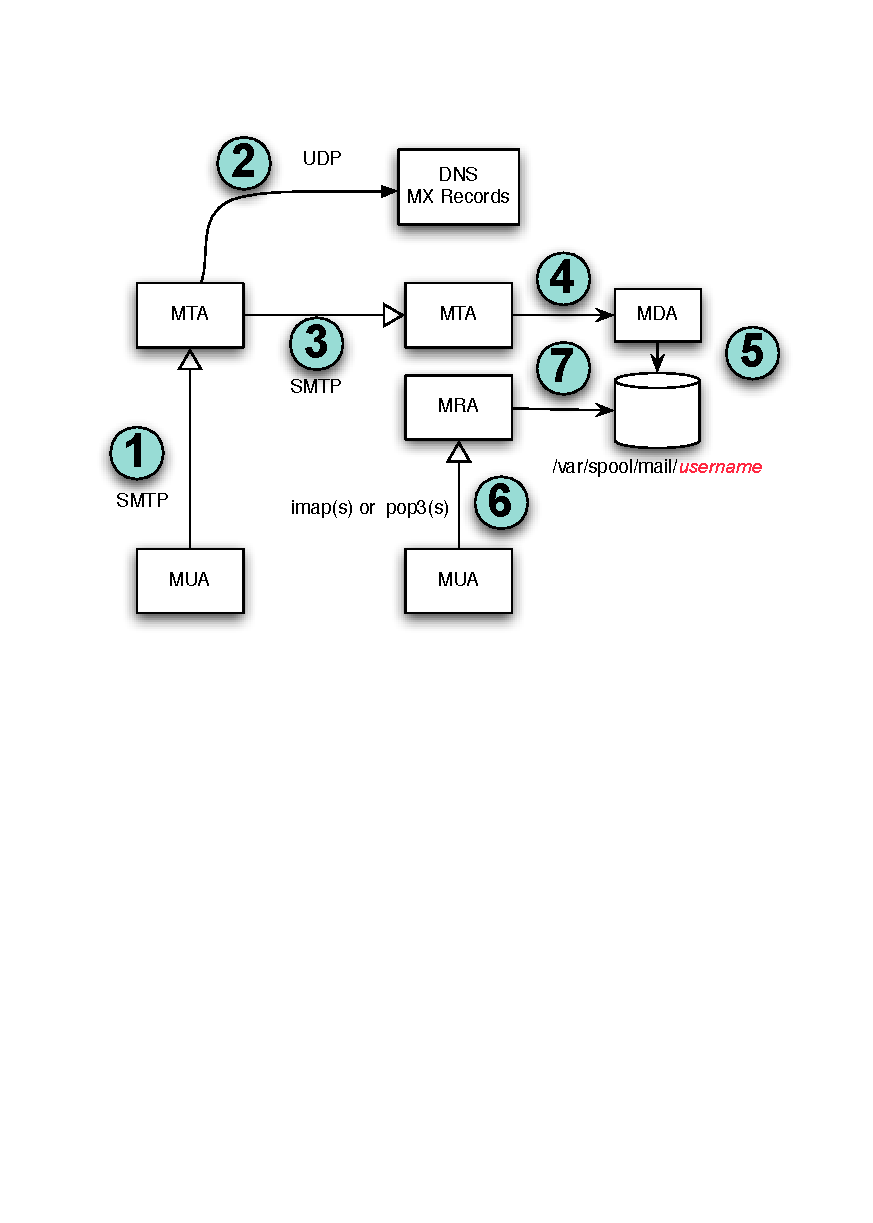
\includegraphics[scale=.8]{images/email-overview}


\end{frame} 
\subsection{smtp协议}


\begin{frame}{Simple Mail Transport Protocol(SMTP)}
\begin{itemize}
\item 和MTA交互的RFC标准协议

\begin{itemize}
\item 通常使用25号TCP端口
\item 扩展SMTP(ESMTP)提供了针对MTA的一些增强特性
\item MTA经常使用LMTP(Local Mail Transport Protocol)来和自己交互
\end{itemize}
\item 明文传送
\item MSP(Message Send Protocol) 例子

\begin{itemize}
\item mail -vs 'some subject ' \emph{username@localhost.localdmain}
\end{itemize}
\item 用telnet排查SMTP连接故障
\end{itemize}

\end{frame} 
\begin{frame}{SMTP协议的使用}
\begin{itemize}
\item SMTP协议命令

\begin{itemize}
\item HELO 通报来访者地址
\item MAIL FROM 发件人地址
\item RCPT TO 收件人地址
\item DATA 输入正文内容,用单独的.为行结束
\item QUIT 连线结束
\end{itemize}
\end{itemize}

\end{frame} 
\begin{frame}{安全与反垃圾邮件策略}
\begin{itemize}
\item 安全策略

\begin{itemize}
\item 拒绝从无法解析的域送来的邮件
\item 建立各种基于主机、用户、域的访问控制
\item 默认配置仅允许本地收发
\item 不再使用setuid的工具
\end{itemize}
\item 反垃圾邮件策略

\begin{itemize}
\item 默认情况下不做转发
\item 建立访问数据库
\item 检查邮件信头
\end{itemize}
\end{itemize}

\end{frame} 
\begin{frame}{Mail Transport Agent(MTA)}
\begin{itemize}
\item 系统默认提供两个MTA

\begin{itemize}
\item sendmail
\item postfix(缺省)
\end{itemize}
\item 通用特性

\begin{itemize}
\item 支持虚拟主机
\item 提供投递失败重试
\item 和spamassassin协作
\end{itemize}
\item 缺省访问控制

\begin{itemize}
\item sendmail/postfix没有setuid组件
\item 仅侦听在本地回路上
\item 转发禁止
\end{itemize}
\end{itemize}

\end{frame} 
\subsection{sendmail概述}

\begin{frame}{sendmail服务一览}

类型:SysV管理的服务

软件包:sendmail,sendmail-cf,sendmail-doc

守护进程:/usr/sbin/sendmail

脚本:/etc/init.d/sendmail

端口:25(smtp)

配置:/etc/mail/sendmail.mc,/etc/aliases,\ldots{}

相关:procmail(MDA),spamassassin,tcp\_wrappers


\end{frame} 
\subsection{sendmail配置}


\begin{frame}{sendmail 配置介绍}
\begin{itemize}
\item 使用和推荐m4 宏语言

\begin{itemize}
\item dnl <space> 表示注释
\end{itemize}
\item service sendmail restart 使用/etc/mail/Makefile

\begin{itemize}
\item /etc/mail/sendmail.mc转为/etc/mail/sendmail.cf
\item 重新hash多个文本数据库
\item make比较时间戳,可以touch一个文件来强制重建/重新hash
\end{itemize}
\item sendmail-cf 缺省并不安装
\item init脚本并不重建文件,除非安装了sendmail-cf软件包
\end{itemize}

\end{frame} 
\begin{frame}{sendmail 流入配置}
\begin{itemize}
\item 修改/etc/mail/sendmail.mc,侦听所有网络接口\\
dnl DEAMON\_OPTIONS(`Port=smtp,Address=127.0.0.1,Name=MTA')dnl
\item 服务器可能提及到的主机名都加入到/etc/mail/local-host-names里
\item 修改访问控制

\begin{itemize}
\item 跟新/etc/hosts.\{allow,deny\}
\item 增加防火墙规则,允许SMTP传输
\end{itemize}
\item 重启sendmail
\end{itemize}

\end{frame} 
\begin{frame}{sendmail 流出配置}
\begin{itemize}
\item 缺省配置 /etc/mail/submit.cf

\begin{itemize}
\item 几乎不要修改
\item 可以把sendmail当作客户端MSP
\end{itemize}
\item 伪装成域,而不是单个主机

\begin{itemize}
\item 取消/etc/mail/sendmail.mc下面几行的注释\\
EXPOSED\_USER(`root')dnl\\
FEATURE(masquerade\_envelope)dnl\\
MASQUERADE\_AS(`example.com')dnl\\
FEATURE(masquerade\_entire\_domain)dnl
\item 这些选项和带外地址重写结合一起工作
\end{itemize}
\end{itemize}

\end{frame} 
\begin{frame}{/etc/aliases}
\begin{itemize}
\item 定义本地用户的别名
\item 别名后的映射对象可以是:

\begin{itemize}
\item 一个本地用户
\item 多个本地用户(用逗号分隔)
\item 本地文件(需要指出路径)
\item 指令(需要管道)
\item 另一个email地址
\end{itemize}
\item 设定完/etc/aliases后,需要运行newaliases更新aliases.db
\end{itemize}

\end{frame} 
\begin{frame}{/etc/virtusertable}


\begin{itemize}
\item 允许在邮件服务中使用虚拟域及虚拟用户并自动映射:\\
joe@abc.com joe\\
@wenhua.org root@wenhua.org \\
eddy@msn.com eddy@wenhua.org
\end{itemize}

\end{frame} 
\begin{frame}{/etc/mail/access}
\begin{itemize}
\item 用于定义接受或拒绝的邮件来源:
\item 格式:\\
IP/域名 设定值
\item 设定值:

\begin{itemize}
\item REJECT:拒绝
\item OK:无条件接受
\item RELAY:允许转发
\item DISCARD:丢弃
\end{itemize}
\end{itemize}

\end{frame} 
\begin{frame}{带外(outbound)地址重写}
\begin{itemize}
\item 在/etc/mail/sendmail.mc里增加下面几行\\
FEATURE(genericstable)dnl\\
FEATURE(`always\_add\_domain')dnl\\
GENERICS\_DOMAIN\_FILE(`/etc/mail/local-host-names')dnl
\item 创建和填充/etc/mail/genericstable\\
paul@example.com paul@otherexample.com\\
david@example.com david.lastname@example.com
\item 域必须在/etc/mail/local-host-names列出
\item 地址重写只对SMTP有效,对LMTP无效
\end{itemize}

\end{frame} 
\begin{frame}{sendmail SMTP 限制}
\begin{enumerate}
\item 在/etc/mail/sendmail.mc里加入下面一行激活\\
FEATURE(`blacklist\_recipients')dnl
\item 在/etc/mail/access里加入限制:\\
From:90trialspammer@aol.com REJECT


Connect:spamRus.net REJECT


Connect:204.168.23 REJECT


Connect:10.3 OK


From:virtualdomain1.com RELAY


To:user@dom9.com ERROR:550 mail discarded


To:nobody@ ERROR:550 bad name

\end{enumerate}
\begin{itemize}
\item 使用标签(tag)来表明黑名单是对sender,recipient还是MTA有效
\item 没有标签的条目发对使用
\end{itemize}

\end{frame} 
\begin{frame}{sendmail 操作}
\begin{itemize}
\item /etc/mail/local-host-names

\begin{itemize}
\item 必须包含服务器主机名和别名
\end{itemize}
\item mail -v \emph{user}

\begin{itemize}
\item 查看本地转发的SMTP交换
\end{itemize}
\item mailq/mailq -Ac

\begin{itemize}
\item 查看将要将要投递的队列
\end{itemize}
\item sendmail -q

\begin{itemize}
\item 重新处理邮件队列
\end{itemize}
\item tail -f /var/log/maillog

\begin{itemize}
\item 实时查看日志
\end{itemize}
\end{itemize}


\subsection{postfix概述}


\end{frame} 
\begin{frame}{postfix服务一览}
\begin{itemize}
\item 类型:SysV管理的服务
\item 软件包:postfix
\item 守护进程:/usr/libexec/postfix/master,其他
\item 脚本:/etc/init.d/postfix
\item 端口:25(smtp)
\item 配置:/etc/postfix/mail.cf,其他
\item 相关:procmail
\end{itemize}

\end{frame} 
\subsection{postfix配置}


\begin{frame}{postfix配置介绍}
\begin{itemize}
\item /etc/postfix/main.cf

\begin{itemize}
\item 良好的注释,采取key=values对形式,按序出现在需要配置的地方
\item 一行开头的空白表示上一行的延续
\item 前面的是可以被作为后面key值序列的变量使用\\
key1=value1\\
key2=\$key1,value2
\end{itemize}
\item postconf

\begin{itemize}
\item 显示设置:postconf -d
\item 显示当前非缺省设置:postconf -n
\item 修改main.cf: postconf -e \emph{key=value}
\item 显示支持的映射类型: postconf -m
\end{itemize}
\end{itemize}

\end{frame} 
\begin{frame}{postfix 流入配置}
\begin{itemize}
\item 修改/etc/postfix/main.cf

\begin{itemize}
\item 监听在所有接口上\\
inet\_interfaces = all
\item 指定服务器可能参考的每一个主机名和别名\\
mydestination = \$myhostname, localhos.\$mydomain,localhost, \$mydomain
\end{itemize}
\item 增加防火墙规则,允许SMTP传输
\item 重启postfix
\item postfix 流出配置
\item 缺省配置提供

\begin{itemize}
\item postfix可以充当MSP客户端
\item 不再需要对单个主机做更多的配置
\item postfix自动解析本地主机名和域名
\end{itemize}
\item 伪装成域名

\begin{itemize}
\item myorigin = \$mydomain


masquerade\_exceptions = root

\end{itemize}
\end{itemize}

\end{frame} 
\begin{frame}{带内postfix别名}
\begin{itemize}
\item 本地别名 /etc/aliases,和sendmail一致
\item 虚拟别名

\begin{enumerate}
\item 在main.cf激活\\
virtual\_alias\_maps = hash:/etc/postfix/virtual
\item 在/etc/postfix/virtual定义,使用和sendmail(virtusertable)同样的格式
\item 重新hash文件: postmap /etc/postfix/virtual
\end{enumerate}
\end{itemize}

\end{frame} 
\begin{frame}{带外地址重写}
\begin{enumerate}
\item 在/etc/postfix/main.cf里激活

\begin{enumerate}
\item smtp\_generic\_maps = hash:/etc/postfix/generic
\end{enumerate}
\item 在/etc/postfix/generic定义\\
paul@example.com paul@otherexample.com\\
david@example.com david.lastname@example.com
\item 重新hash文件:postmap /etc/postfix/generic
\end{enumerate}

\end{frame} 
\begin{frame}{postfix 限制}
\begin{enumerate}
\item 创建/etc/postfix/access

\begin{itemize}
\item /etc/mail/access的无标签版本
\item 重新hash postmap /etc/postfix/access
\end{itemize}
\item 编辑main.cf\\
smtpd\_TAG\_restrictions =\\
check\_TAG\_access hash:/etc/postfix/access, \ldots{}

\begin{itemize}
\item TAG是sender,recipient,client中的一个
\item 例子\\
smtpd\_recipient\_restrictions =


check\_recipient\_access hash:/etc/postfix/access,


permit\_mynetworks, reject\_unauth\_destination

\end{itemize}
\end{enumerate}

\end{frame} 
\begin{frame}{postfix 操作}
\begin{itemize}
\item main.cf 设置

\begin{itemize}
\item 服务器名:mydestinatio 必须包含服务器的名字和别名
\item 监听接口:inet\_interfaces = all
\item 归档所有邮件:always\_bcc = \emph{address}
\end{itemize}
\item 查看SMTP交换:mail -v user@domain.tld
\item 查看延期的邮件:postqueue -p
\item 清空延期的邮件:postqueue -f
\item 实时查看日志:tail -f /var/log/maillog
\end{itemize}

\end{frame} 
\subsection{Procmail 概述}

\begin{frame}{Procmail,邮件投递代理(Mail Delivery Agent)}
\begin{itemize}
\item 不同的使用,包括

\begin{itemize}
\item 对收到来信进行排序,并送入不同目录或者文件
\item 预处理邮件
\item 邮件达到后,开启一个事件或者程序
\item 自动转发邮件给其他人
\end{itemize}
\item 激活 procmail

\begin{itemize}
\item sendmail:缺省激活
\item postfix:修改 /etc/postfix/main.cf\\
mailbox\_command = /usr/bin/procmail
\end{itemize}
\item 有可能在短时间内产生大量转发邮件,因此配置时应小心谨慎
\end{itemize}

\end{frame} 
\begin{frame}{Procmail和访问控制}
\begin{itemize}
\item 初始化控制

\begin{itemize}
\item Procmail以 nobody 帐号运行
\item Procmail属于 mail 组
\item /var/spool/mail 仅对 root 和 mail 组可写
\end{itemize}
\item 要求:改变procmail程序以setgid方式运行\\
chmod g+s \$(which procmail)
\end{itemize}

\end{frame} 
\subsection{procmail 配置}


\begin{frame}{procmail 配置介绍}
\begin{itemize}
\item 配置文件按序处理

\begin{enumerate}
\item /etc/procmailrc
\item \textasciitilde{}/.procmailrc
\end{enumerate}
\item 配置文件里的元素

\begin{itemize}
\item 指令: VERBOSE=yes
\item 变量:LOGFILE=/var/spool/mail/procmail.log
\item 处理

\begin{itemize}
\item 一行以':0'开始
\item 零或多个匹配行使用正规表达式
\item 一行或多行动作
\end{itemize}
\end{itemize}
\end{itemize}

\end{frame} 
\begin{frame}{Procmail 处理实例}
\begin{itemize}
\item 将来自wgzhao关于linux的邮件转发给lancy,并复制到linux目录\\
:0


{*}\textasciicircum{}From.{*}wgzhao


{*}\textasciicircum{}Subject:.{*}linux


\{ :0 c


! todd@xplore.cn


:0


linux


\}

\item man手册:procmailex,procmailrc,procmail
\end{itemize}

\end{frame} 
\subsection{邮件接收}


\begin{frame}{Mail Retrieval Protocols}
\begin{itemize}
\item 邮局协议 Post Office Protocols

\begin{itemize}
\item 所有的数据,包括密码,通过TCP 110端口明文传输
\item 使用POP3s对在TCP 995端口上传输的数据提供了SSL加密
\end{itemize}
\item 交互邮件访问协议 Internet Mail Access Protocol

\begin{itemize}
\item 所有的数据,包括密码,通过TCP 143端口明文传输
\item 使用POP3s对在TCP 993端口上传输的数据提供了SSL加密
\end{itemize}
\item Dovecot 支持POP3,POP3s,IMAP和IMAPs
\end{itemize}

\end{frame} 
\subsection{配置dovecot}


\begin{frame}{Dovecot服务一览}
\begin{itemize}
\item 类型:SysV管理的服务
\item 软件包:dovecot
\item 守护进程:/usr/sbin/dovecot
\item 脚本:/etc/init.d/dovecot
\item 端口:110(pop3),995(pop3s),143(imap),993(imaps)
\item 配置:/etc/dovecot.conf
\item 相关:procmail,fetchmail,openssl
\end{itemize}

\end{frame} 
\begin{frame}{Dovecot 配置}
\begin{itemize}
\item 缺省监听在所有的IPv6和IPv4接口上
\item 在/etc/dovecot.conf里指定协议

\begin{itemize}
\item protocols = imap imaps pop3 pop3s
\end{itemize}
\item 使用SSL之前创建私钥和自签名证书

\begin{enumerate}
\item 确认系统时间以免时钟问题
\item 检查/etc/dovecot.conf里配置密钥和证书的位置
\item 运行 make -C /etc/pki/tls/certs dovecot.pem

\begin{itemize}
\item 创建单个PEM文件同时包含密钥和证书
\end{itemize}
\item 拷贝新的PEM文件到定义密钥和证书的位置
\end{enumerate}
\end{itemize}

\end{frame} 
\begin{frame}{校验POP操作}
\begin{itemize}
\item 校验服务器操作

\begin{itemize}
\item 图形化工具:Thundbird,kmail,\ldots{}
\item 文字模式:mutt,fetchmail\\
mutt -f pop://user@server{[}:port{]}\\
mutt -f pops://user@server{[}:port{]}
\item 可以使用telnet(pop3)或者openssl s\_client (pop3s)
\end{itemize}
\end{itemize}

\end{frame} 
\begin{frame}{校验IMAP操作}
\begin{itemize}
\item 校验服务器操作

\begin{itemize}
\item 图形化工具:Thundbird,kmail,\ldots{}
\item 文字模式:mutt,fetchmail\\
mutt -f imap://user@server{[}:port{]}\\
mutt -f imaps://user@server{[}:port{]}
\end{itemize}
\item 也可以使用telnet(IMAP)或openssl s\_client(IMAPs)
\end{itemize}

\end{frame} 
\subsection{邮件服务实验}


\begin{frame}{实验I:配置sendmail为MTA}
\begin{description}
\item [{场景:}] 一个站点需要一个本地的邮件服务器来支持,域名为example.com。考虑安全实现
\item [{要求:}] 为example.com提供sendmail邮件服务
\end{description}
提示
\begin{enumerate}
\item 默认sendmail仅接受本地回路请求
\item 和DNS结合
\item 考虑防火墙
\end{enumerate}

\end{frame} 
\begin{frame}{实验II:迁移到postfix}
\begin{description}
\item [{场景:}] 使用sendmail的设备决定迁移到postfix来提供邮件服务。安装和实现它,适当考虑安全。
\item [{要求:}] 为example.com提供postfix邮件服务
\end{description}

\end{frame} 
\begin{frame}{实验III:增加新的别名}
\begin{description}
\item [{场景:}] 你的机构需要一一系列常用的email帐号,他们会重定向到实际用户帐号。使用邮件别名实现这个特性
\item [{要求:}] 邮件别名分布系统
\end{description}

\end{frame} 
\begin{frame}{实验IV:安装Dovecot作为MRA}
\begin{description}
\item [{场景:}] 远程用户需要访问在本地服务器上的邮件。配置Dovecot,允许所有邮件获取协议的连接,加密协议使用缺省证书。
\item [{要求:}] 配置MRA功能服务器
\end{description}
提示
\begin{enumerate}
\item 首先实现非加密协议的邮件获取
\item 后实现加密协议的邮件获取
\item 选择好的MUA或者命令行工具来调试
\end{enumerate}

\end{frame} 
\begin{frame}{实验V:创建唯一的Dovecot证书}
\begin{description}
\item [{场景:}] 对从非安全协议嗅探密码的担忧,决定使用特定站点的加密证书
\item [{要求:}] 实现MRA安全服务
\end{description}
提示
\begin{enumerate}
\item Dovecot 安装时,提供了通用的加密key,他们可能会遭遇中间人(man in the middle)攻击。
\item 考虑系统提供的key /etc/pki/tls/certs
\item make -C /etc/pki/tls/certs dovecot.pem
\end{enumerate}

\end{frame}


%
%\part{安全}


%\section{安全概述}

% \begin{frame}{安全策略}
%	\tableofcontents[currentsection]
%
%%
%%目标
%%\begin{itemize}
%%\item 理解系统性能安全目标
%%\item 解释维护系统状态的好处
%%\item 描述网络资源
%%\item 描述数据存储资源
%%\item 描述进程资源
%%\item 描述日志分析
%%\end{itemize}
%
%\end{frame} 

%\subsection{安全原则}
%
%
% \begin{frame}{安全原则}
%\begin{itemize}
%\item 物理安全
%\item 本地安全
%\item 远程安全
%\item 个人安全
%\end{itemize}
%
%\end{frame} 
%\begin{frame}{安全实践}
%\begin{itemize}
%\item 经过设计,系统通过有效的资源服务
%\item 根据策略,系统保护有效的资源
%\item 主机应该仅提供必须的服务,以及提供那些必须的人
%
%\begin{itemize}
%\item 我需要或者知道主机提供了什么吗?
%\item 他们需要或者知道访问这些服务吗?
%\item 系统行为和记录一致吗?
%\item 应用了所有相关安全补丁吗?
%\end{itemize}
%\item 监控系统资源,了解系统性能以及漏洞
%\end{itemize}
%
%\end{frame} 
%
%
% \begin{frame}{安全策略:人}
%\begin{itemize}
%\item 管理人的活动
%\item 谁管理什么
%\item 谁能对虚假警报做最终决定
%\item 什么时候可以通知执法机关
%\end{itemize}
%
%\end{frame} 
%
%
% \begin{frame}{安全策略:系统}
%\begin{itemize}
%\item 管理系统活动
%\item 常规系统监控
%
%\begin{itemize}
%\item 日志记录到一台外部服务器,以防出现意外
%\item 使用logwatch 监控日志
%\item 监控网络带宽的出站和进站使用情况
%\end{itemize}
%\item 系统数据常规备份
%\end{itemize}
%
%\end{frame} 
%
%
% \begin{frame}{应答策略}
%\begin{itemize}
%\item 假定可疑系统是不值得信任的
%
%\begin{itemize}
%\item 不要从可疑系统上运行程序
%\item 从可信赖介质启动,校验问题
%\item 分析远程日志服务器记录的日志以及“本地”日志
%\item 从RPM数据库的只读备份里检查文件完善性
%\end{itemize}
%\item 对当前机器做一个镜像,以便将来继续分析或者搜索证据
%\item 清除系统,重新安装,如何从备份中恢复你需要的数据
%\end{itemize}
%\end{frame} 

\section{系统安全}
\begin{frame}{系统安全}
\tableofcontents[currentsection]
\end{frame}
 
 \subsection{系统监控}

\begin{frame}{系统监控的好处}
\begin{itemize}
\item 通过常规监控,系统虚拟和安全得以维护
\item 系统监控包括

\begin{itemize}
\item 网络监控和分析
\item 文件系统监控
\item 进程监控
\item 日志文件分析
\end{itemize}
\end{itemize}

\end{frame} 

 \begin{frame}{网络监控工具}
\begin{itemize}
	\item 网络接口(ip)
	
	\begin{itemize}
		\item 显示系统上有效的网络接口
	\end{itemize}
	\item 端口扫描(nmap)
	
	\begin{itemize}
		\item 显示系统提供了哪些有效服务
	\end{itemize}
	\item 包嗅探(tcpdump,wireshark)
	
	\begin{itemize}
		\item 保存和分析所有网络通信到'嗅探'系统上
	\end{itemize}
\end{itemize}

\end{frame} 

\begin{frame}{查看本地网络}
\begin{itemize}
\item ip 工具

\begin{itemize}
\item 初始化脚本调用
\item 比ifconfig功能更强
\end{itemize}
\item netstat -ntaupe 列出

\begin{itemize}
\item 活动的网络服务
\item 已建立的连接
\end{itemize}
\end{itemize}

\end{frame} 

\begin{frame}{查看远程网络}
\begin{itemize}
\item nmap 报告开放端口上的服务

\begin{itemize}
\item 有效的高级扫描选项
\item 提供远程OS探测(-O)
\item 大小子网均可扫描
\end{itemize}
\item 管理员权限下使用
\item 图形化前端程序可用(zenmap\footnote{\href{http://nmap.org/zenmap/}{http://nmap.org/zenmap}}/nmapsi4\footnote{\href{http://nmapsi4.netsons.org/web/}{http://nmapsi4.netsons.org/web/}})
\end{itemize}

\end{frame} 


 \begin{frame}{文件系统分析}
\begin{itemize}
\item 常规文件系统监控可以防止

\begin{itemize}
\item 系统资源耗尽
\item 因为缺乏访问控制而导致的系统突破点
\end{itemize}
\item 文件系统监控应该包括

\begin{itemize}
\item 数据完整性扫描
\item 可疑文件调查
\end{itemize}
\item 工具

\begin{itemize}
\item df,du
\end{itemize}
\end{itemize}

\end{frame} 


 \begin{frame}{典型的有问题的许可}
\begin{itemize}
\item 未知属主的文件可能表明系统遇到非授权访问

\begin{itemize}
\item 查看没有用户或者组的文件\\
find / -nouser -o -nogroup 
\end{itemize}
\item 文件/目录对任何人有写(o+w)许可,表示可能有问题

\begin{itemize}
\item 定位这些文件\\
find / -type f -perm -002
\item 定位这些目录\\
find / -type d -perm -002
\end{itemize}
\end{itemize}

\end{frame} 


 \begin{frame}{监控进程}
\begin{itemize}
\item 监控进程来决定

\begin{itemize}
\item 性能降低的原因
\item 可疑进程是否存在
\end{itemize}
\item 监控工具

\begin{itemize}
\item top
\item gnome-system-monitor
\item sar,rfsar
\end{itemize}
\end{itemize}

\end{frame} 
 \begin{frame}{进程监控工具}
\begin{itemize}
\item top

\begin{itemize}
\item 实时查看活动进程
\item 交互模式下杀死进程或者调整进程优先级(renice)
\item 观察系统统计数据的更新
\end{itemize}
\item GUI 监控工具

\begin{itemize}
\item gnome-system-monitor: 进程,CPU,内存监控
\item kpm: top的KDE版
\item rfsar: sar的图形化实现
\end{itemize}
\end{itemize}

\end{frame} 

% \begin{frame}{系统活动报告}
%\begin{itemize}
%\item 频繁报告
%
%\begin{itemize}
%\item cron spawns sa1,sa2
%\item sar 读取日志,生成人可读的日志
%\end{itemize}
%\item 通常用户性能调试
%
%\begin{itemize}
%\item 更多精确的统计
%
%\begin{itemize}
%\item 二进制数据库收集方法
%\item 正常时间间隔
%\end{itemize}
%\end{itemize}
%\end{itemize}
%
%\end{frame} 

% \begin{frame}{通过帐号管理进程}
%\begin{itemize}
%\item 使用PAM来控制某一个帐号的资源限制
%
%\begin{description}
%\item [{pam\_access.so}] 可以通过帐号和位置来限制访问
%\item [{pam\_time.so}] 通过日期和时间显示访问
%\item [{pam\_limits.so}] 可以限制某一个进程的有效资源
%\end{description}
%\end{itemize}
%
%\end{frame} 
% \begin{frame}{系统日志文件}
%\begin{itemize}
%\item 为什么要监控日志文件
%\item 哪些日志需要监控
%\item 日志服务
%
%\begin{itemize}
%\item 大部分守护进程发送消息到syslogd
%\item 内核消息由klogd处理
%\end{itemize}
%\end{itemize}
%
%\end{frame} 
% \begin{frame}{syslogd/klogd 配置}
%\begin{itemize}
%\item 配置文件 /etc/syslog.conf
%\item 语法:\\
%\emph{facility.priority log\_location}
%\item 实例\\
%mail.info /dev/tty8
%\end{itemize}
%
%\end{frame} 


% \begin{frame}{日志文件分析}
%\begin{itemize}
%\item 对常规部分进行分析
%\item logwatch 可以通过cron来运行,每小时来报告可能的问题
%\item 当查找反常信息时,logwatch 使用negative lists
%
%\begin{itemize}
%\item 丢失所有正常的信息
%\item 分析剩余的
%\end{itemize}
%\end{itemize}
%
%
%\end{frame} 

%\section{帐号安全管理}

%
%%
%% \begin{frame}{帐号安全管理}
%%目标
%%\begin{itemize}
%%\item 理解基本认证
%%\item 掌握sudo的配置
%%\item 理解NSS和PAM的角色
%%\end{itemize}
%%\end{frame} 
%
%
% \subsection{帐号概述}
%
%
%
% \begin{frame}{用户帐号}
%\begin{itemize}
%\item 对每一个用户帐号而言必须提供两类信息
%
%\begin{itemize}
%\item 帐号信息
%
%\begin{itemize}
%\item UID,缺省shell,家目录,组成员等
%\end{itemize}
%\item 认证
%
%\begin{itemize}
%\item 登录时,如何告知提供给登录的密码是正确的实现方法
%\end{itemize}
%\end{itemize}
%\end{itemize}
%\end{frame} 
%
%\begin{frame}{帐号信息(名称服务器)}
%\begin{itemize}
%\item 名称服务器通过访问库函数来映射名字到账户信息
%\item 最初,名称服务器仅由本地文件,比如/etc/passwd,来提供
%\item 后来通过重写libc增加了新的成名服务器,比如NIS的支持
%\end{itemize}
%
%\end{frame} 
% \begin{frame}{名称服务器交换(NSS)}
%\begin{itemize}
%\item NSS可以在不重写libc的情况下增加新的名称服务器
%
%\begin{itemize}
%\item 使用/lib/libnss\_service.so 文件
%\end{itemize}
%\item /etc/nsswitch.conf 控制以名称服务器以什么顺序来检查
%
%\begin{itemize}
%\item passwd: files nis ldap
%\end{itemize}
%\end{itemize}
%
%\end{frame} 
%
%%\begin{frame}{getent}
%%\begin{itemize}
%%\item getent \textit{database}
%%
%%\begin{itemize}
%%\item 列出指定数据库存储的所有对象
%%\item getent \textit{services}
%%\end{itemize}
%%\item getent \textit{database name}
%%
%%\begin{itemize}
%%\item 在指定数据里,查询指定名字的信息
%%\item getent passwd wgzhao
%%\end{itemize}
%%\end{itemize}
%%
%%\end{frame} 
%
%\begin{frame}{认证}
%\begin{itemize}
%\item 应用程序认证密码的传统做法是通过libc函数
%
%\begin{itemize}
%\item 对登录是提供的密码进行哈希
%\item 在NSS比较哈希后的密码
%\item 如果匹配,认证通过
%\end{itemize}
%\item 一旦认证方法改动,应用程序必须重写
%\end{itemize}
%\end{frame} 
%
% \subsection{sudo}
%
% \begin{frame}{sudo}
%\begin{itemize}
%\item 在/etc/sudoers文件里包含的账户,执行指令时:
%
%\begin{itemize}
%\item euid为0,而不是uid
%\item gid是root组的id,而不是私有组的id
%\end{itemize}
%\item 非/etc/sudoers里包含的账户企图执行sudo指令时,会通知要求和管理员(root)联系
%\item url:{} \href{http://blog.wgzhao.com/2009/03/13/using-sudo-effectively.html}{如何用好sudo}
%\end{itemize}
%\end{frame} 


%\subsection{PAM概述}
%
%
%
% \begin{frame}{Pluggable Authentication Modules(PAM)}
%\begin{itemize}
%\item Pluggable Authentication Modules 可植入认证模块
%\item 应用程序调用libpam函数认证和授权用户
%\item libpam复杂检查应用程序的PAM配置文件
%
%\begin{itemize}
%\item 可能会包括NSS检查
%\end{itemize}
%\item 共享的,动态配置代码
%\item 文档: /usr/share/doc/pam-<version>/
%\end{itemize}
%
%\end{frame} 
% \begin{frame}{PAM 操作}
%\begin{itemize}
%\item /lib/security/ PAM 模块
%
%\begin{itemize}
%\item 每一个模块执行一个测试,通过或者失败
%\item /etc/security/ 下的文件可能一些模块应该如何执行测试
%\end{itemize}
%\item /etc/pam.d/ PAM配置文件
%
%\begin{itemize}
%\item 这些文件决定如何以及何时模块被特定应用程序使用
%\end{itemize}
%\end{itemize}
%\end{frame} 
%
% \subsection{PAM配置}
%
%
%
% \begin{frame}{/etc/pam.d/ 文件: 测试}
%\begin{itemize}
%\item 测试组织成下面四个组:
%
%\begin{description}
%\item [{auth}] 认证这个用户就是那个用户
%\item [{account}] 授权帐号可以使用什么
%\item [{password}] 控制密码改变
%\item [{session}] 打开,关闭,记录会话
%\end{description}
%\item 每一个组根据需要被调用,并提供单独的结果给服务器
%\end{itemize}
%
%\end{frame} 
%
% \begin{frame}[shrink]{/etc/pam.d/ 文件:控制值}
%\begin{itemize}
%\item 控制值(Control values)决定每一个测试结果如何影响整个组的总结果
%
%\begin{description}
%\item [{required}] 模块检查必须成功,验证过程才能继续。如果当前模块检查失败,则只有当使用相同模块接口的所有模块都检查之后,当前模块的检查结果才会通知用户; 
%\item 
%\item [{requisite}] 模块检查必须成功,验证过程才能继续。不过,如果当前模块检查失败,会立即通知用户,并且返回一条第一个required或者requisite模块检查失败时输出的错误信息; 
%\item [{sufficient}] 如果模块检查失败,则这个结果会被忽略。不过,如果当前模块检查成功,同时之前没有其它的sufficient模块检查失败,则验证过程不会继续检查其它模块,用户通过验证; 
%\item [{optional}] 模块检查返回的结果被忽略。optional的模块只有在整个验证过程中没有其它的模块使用这个模块所引用的接口时才会对验证结果起作用。 
%\end{description}
%\end{itemize}
%
%\end{frame} 
% 
% \begin{frame}[fragile]{实例 /etc/pam.d/login 文件}
%
%\verbatiminput{/etc/pam.d/login}
%
%\end{frame} 
%
%\begin{frame}{system-auth 文件}
%\begin{itemize}
%	\item system-auth被广泛使用
%	\item 通过include 控制标志来调用,并不是作为一个模块(比如pam\_stack.so)
%	\item 包含标准认证测试
%	\item 可以共享给系统上的许多应用程序
%	\item 使得系统标准认证管理简单且一致
%\end{itemize}
%\end{frame}
%
% \begin{frame}{pam\_unix.so}
%\begin{itemize}
%\item 针对基于NSS的认证模块
%
%\begin{description}
%\item [{auth}] 从NSS获得哈希密码并和输入的密码哈希后进行比较
%\item [{account}] 检查密码过期
%\item [{password}] 处理本地文件或者NIS密码更改
%\item [{session}] 记录登入和登出到日志
%\end{description}
%\end{itemize}
%
%\end{frame} 
% \begin{frame}{网络认证}
%\begin{itemize}
%\item 集中密码管理
%
%\begin{description}
%\item [{pam\_krb5.so}] Kerberos 第五版许可证
%\item [{pam\_ldap.so}] LDAP 绑定
%\item [{pam\_smb\_auth.so}] 老的SMB认证
%\item [{pam\_winbind.so}] SMB,通过winbindd
%\end{description}
%\item 有些服务使用NSS/pam\_unix.so
%\end{itemize}
%\end{frame} 
%
%\begin{frame}{auth 模块}
%\begin{itemize}
%\item pam\_securetty.so 如果root帐号从没列在/etc/securetty里的终端登录,则认证失败
%\item pam\_nologin.so 如果用户不是root且文件/etc/nologin存在,则认证失败
%\item pam\_listfile.so 依据某一个文件内容列表来做认证字符检查
%
%\begin{itemize}
%\item 列出帐号可以允许或者拒绝
%\end{itemize}
%\end{itemize}
%
%\end{frame} 
% \begin{frame}{密码安全}
%\begin{itemize}
%\item pam\_unix.so MD5 密码哈希
%
%\begin{itemize}
%\item 密码哈希,难于破解
%\end{itemize}
%\item pam\_unix.so 影子密码
%
%\begin{itemize}
%\item 密码哈希,仅对root可见
%\item 设置密码有效期限
%\end{itemize}
%\item 其他模块可能支持密码老化机制
%\end{itemize}
%\end{frame} 
%
% \subsection{密码策略}
%
%
%
% \begin{frame}{密码策略}
%\begin{itemize}
%\item 密码历史
%
%\begin{itemize}
%\item pam\_unix.so 使用remember=\emph{N} 参数
%\end{itemize}
%\item 密码强度
%
%\begin{itemize}
%\item pam\_cracklib.so
%\item pam\_passwdqc.so
%\end{itemize}
%\item 登录失败监控
%
%\begin{itemize}
%\item pam\_tally.so
%\end{itemize}
%\end{itemize}
%
%\end{frame} 
% \begin{frame}{session 模块}
%\begin{itemize}
%\item pam\_limits.so 强制资源限制
%
%\begin{itemize}
%\item 使用/etc/security/limits.conf
%\end{itemize}
%\item pam\_console.so 对终端用户,设置本地设备许可
%\item pam\_selinux.so 帮助设置SELinux上下文
%\item pam\_mkhomedir.so 创建家目录,如果不存在的话
%\end{itemize}
%
%\end{frame} 
% \begin{frame}{使用工具和认证}
%\begin{itemize}
%\item 本地需要认证的管理工具
%
%\begin{itemize}
%\item su,reboot,rf{*},\ldots{}
%\end{itemize}
%\item pam\_rootok.so 如果以root运行,则通过
%\item pam\_timestamp.so 针对类似sudo行为
%\item pam\_xauth.so 转发xauth cookies
%\end{itemize}
%
%\end{frame} 
% \begin{frame}{PAM故障排除}
%\begin{itemize}
%\item 检查系统日志
%
%\begin{itemize}
%\item /var/log/messages
%\item /var/log/secure
%\end{itemize}
%\item PAM的错误可能会导致root无法登录
%
%\begin{itemize}
%\item 测试PAM时,保留一个root登录的窗口
%\item 单用户模式可以绕过PAM
%\item 系统救援模式启动系统
%\end{itemize}
%\end{itemize}
%\end{frame} 

\section{网络安全}

\begin{frame}{网络安全}

%目标
%\begin{itemize}
%%\item 理解tcp\_wrappers
%%\item 使用libwrap.so识别应用程序
%\item 理解iptables 防火墙
%\item 定制iptables防火墙规则
%\end{itemize}
\tableofcontents[currentsection]
\end{frame} 

%\subsection{tcp\_wrappers}
%\begin{comment}
%象Telnet、SSH、FTP、POP和SMTP等很多网络服务都会用到TCP Wrapper,它被设计为一个介于外来服务请求和系统服务回应的中间处理软件。 
%它的基本过程是这样的:当系统接收到一个外来服务请求的时候,先由TCP Wrapper处理这个请求,TCP Wrapper根据这个请求所请求的服务和针对这个服务所定制的存取控制规则来判断对方是否有使用这个服务的权限,如果有,TCP Wrapper将该请求按照配置文件定义的规则转交给相应的守护进程去处理同时记录这个请求动作,然后自己就等待下一个请求的处理。
% TCP Wrapper机制的主要目的在于,来自客户端的请求只被允许同一个独立的守护进程(xinetd)直接通信,而它请求的目标服务被TCP Wrapper包裹起来,这样就提高了系统的安全性和系统管理的方便性。 
%TCP Wrapper 提高了系统的安全性。系统安全性的具体体现主要有两点,一个是获取访问权限前的控制,一个是获取访问后的处理。获取权限前,它会根据/etc/hosts.allow和/etc/hosts.deny定制的规则来判断对方是否有权限;获取权限后,通过bind、redirect等属性的设置,可能已经由另一台主机或者另一个服务在处理了对方的请求,而对方并不会感知中间经过了这样的处理。 
%TCP Wrapper更加方便了系统管理。一方面可以抽取系统所有服务共有的属性放到/etc/xinetd.conf中,另一方面,将每一个服务具体的配置放到/etc/inetd.d目录下,而每个配置文件都遵循同样的语法和规则。  
%TCP Wrapper的功能来自于libwrap.a,它是一个网络服务库,象xinetd、sshd和portmap等许多系统服务编译时都依赖于它,其他的网路服务程序甚至你自己编写的网络服务程序都可以加上这个编译选项来提供TCP Wrapper的功能。
%\end{comment}
%
%\begin{frame}{tcp\_wrappers 配置}
%\begin{itemize}
%\item 访问检查的三个阶段
%
%\begin{itemize}
%\item 访问是否被明确许可
%\item 否则,访问是否被明确拒绝
%\item 如果都没有,默认许可
%\end{itemize}
%\item 配置存储在两个文件里
%
%\begin{itemize}
%\item 许可用: /etc/hosts.allow
%\item 拒绝用: /etc/hosts.deny
%\end{itemize}
%\item 基本语法
%
%\begin{itemize}
%\item \emph{守护进程列表:客户端列表 {[} :参数 {]}}
%\end{itemize}
%\end{itemize}
%
%\end{frame} 
%
%\mode<handout>
%{
%the first fields specifies a comma-delimited list of daemons.tcp_wrappers usually takes argv[0] (process name without path)as the deamon name
%example
%in.telnetd: 192.168.0.1
%sshd,gdm: 192.168.0.1
%if your host has more than one network interface and you want to implement different policies for them,use the following syntax:
%in.telnetd@192.168.0.254: 192.168.0.
%in.telnetd@192.168.1.254: 192.168.1.
%}
%
%\begin{frame}{守护进程列表}
%
%\begin{itemize}
%\item 守护进程列表应该是
%
%\begin{itemize}
%\item 服务的可执行程序名
%\item 允许指定多个服务
%\item 使用ALL 匹配所有服务
%\item 允许可执行程序名后添加IP或主机名,如果本机有多个网络接口
%\end{itemize}
%\item 高级语法
%
%\begin{itemize}
%\item \emph{deamon@host: client\_list \ldots{}}
%\end{itemize}
%\end{itemize}
%
%\end{frame} 
% \begin{frame}{客户端列表}
%
%
%\begin{itemize}
%\item 主机规范
%
%\begin{itemize}
%\item IP地址(192.168.1.1,10.0.0.)
%\item 域名或主机名(www.redflag-linux.com, .wgzhao.com)
%\item 子网掩码(192.168.1.0/255.255.255.0)
%\item 网络名(@mydomain)
%\end{itemize}
%\end{itemize}
%
%\end{frame} 
% \begin{frame}{高级客户端语法}
%\begin{itemize}
%\item 通配符
%
%\begin{itemize}
%\item ALL : 总是匹配
%\item LOCAL:所有名字不包含'.'的主机
%\item KNOWN:可以双向解析的主机或用户
%\item UNKNOWN: 无法被解析的主机或用户
%\item PARANOID:正向解析和反向解析不匹配的主机
%\end{itemize}
%\item EXCEPT
%\mode<handout>
%{
%/etc/hosts.allow
%sshd: ALL EXCEPT .cracker.org EXCEPT trusted.cracker.org
%/etc/hosts.deny
%sshd: ALL
%}
%\begin{itemize}
%\item 可以用于客户端和服务端列表
%\item 可以嵌套使用
%\end{itemize}
%\end{itemize}
%
%\end{frame} 
%
% \begin{frame}{扩充选项}
%\begin{itemize}
%\item 语法\\
%\textit{daemon\_list: client\_list {[} :opt1 :opt2 \ldots{}{]}}
%\item spwan
%
%\begin{itemize}
%\item 用来启动额外程序
%\item 特殊扩展有效(\%c,\%s)
%\end{itemize}
%\item 举例\\
%in.telnetd: ALL : spawn echo `login attempt from \%c to \%s' | mail -s warning root
%\item DENY
%
%\begin{itemize}
%\item 作为可选现用在hosts.allow 里
%\end{itemize}
%\item 举例
%
%\begin{itemize}
%\item ALL: ALL: DENY
%\end{itemize}
%\end{itemize}
%
%\end{frame} 
% \begin{frame}{tcp\_wrappers 例子}
%
%\# /etc/hosts.allow
%
%vsftpd : 192.168.1.
%
%in.telnetd,sshd : .xplore.cn 192.168.2.240
%
%\medskip{}
%
%
%\# /etc/hosts.deny
%
%ALL : ALL
%
%
%\end{frame} 
% \begin{frame}{xinetd和tcp\_wrappers}
%\begin{itemize}
%\item xinetd 提供了自己的一套访问控制
%
%\begin{itemize}
%\item 基于主机
%\item 基于时间
%\end{itemize}
%\item 在xinetd与tcp\_wrapper都限制的情况下
%
%\begin{itemize}
%\item 先检查tcp\_wrapper
%\item 如果tcp\_wrapper允许连接,再检查xinetd是否也允许
%\end{itemize}
%\end{itemize}
%\end{frame} 

\subsection{防火墙}

\begin{frame}{Netfilter 概述}
\begin{itemize}
\item 在内核中过滤,没有守护进程
\item 在OSI参考模型的2,3,4层申明
\item 仅检查包头信息
\item 由内核模块netfilter和用户空间的iptables指令组成
\end{itemize}

\end{frame} 
 \begin{frame}{Netfilter表和链}

\begin{center}
\begin{tabular}{|c|c|c|c|}
\hline 
过滤点(chain) & \multicolumn{3}{c|}{表}\tabularnewline
\cline{2-4} 
 & filter & NAT & mangle\tabularnewline
\hline 
INPUT & X &  & X\tabularnewline
\hline 
FORWARD & X &  & X\tabularnewline
\hline 
OUTPUT & X & X & X\tabularnewline
\hline 
PREROUTING &  & X & X\tabularnewline
\hline 
POSTROUTING &  & X & X\tabularnewline
\hline 
\end{tabular}
\par\end{center}


\end{frame} 
 \begin{frame}{Netfilter 包流程图}
\center
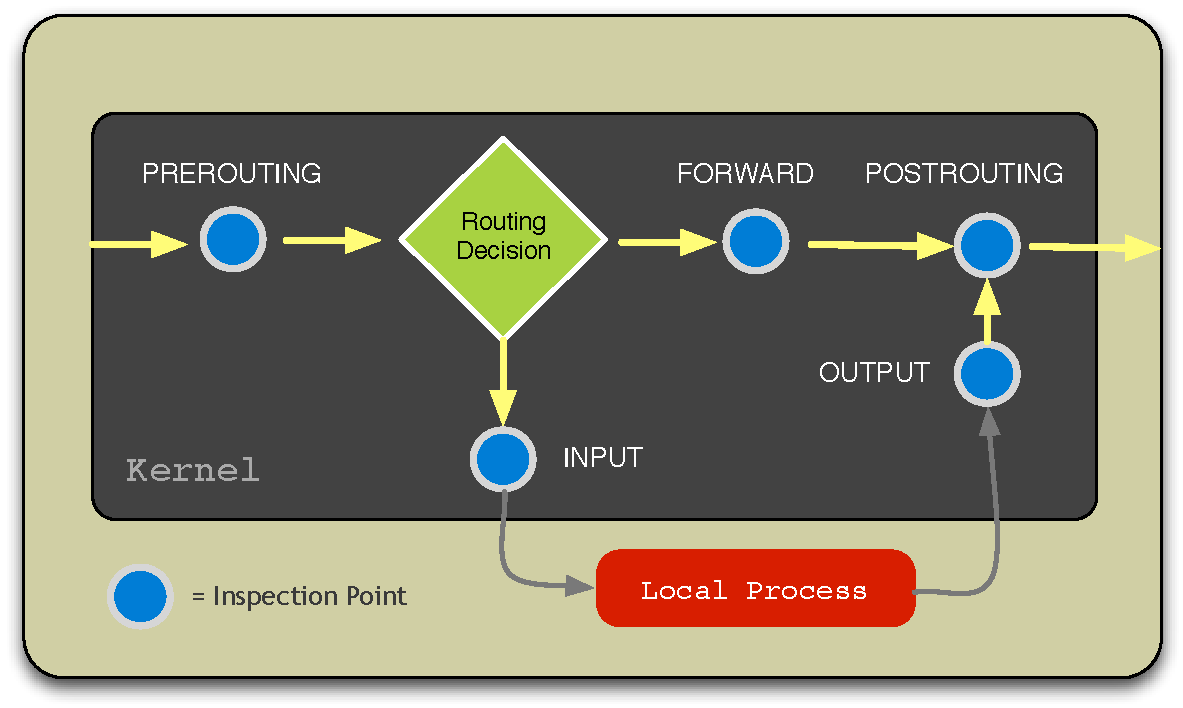
\includegraphics[scale=.6]{netfilter-packet-flow.pdf}
\end{frame} 

\begin{frame}{规则匹配}
\begin{itemize}
\item 规则排序列表
\item 包一次通过每一个规则的测试
\item 首次匹配,目标(target)开始工作:一般是退出链
\item 规则可以指定多个标准用来匹配
\item 规范里的每一个标准必须满足规则匹配
\item 如果没有匹配,则链策略应用
\end{itemize}

\end{frame} 
 \begin{frame}{简单例子}

filter表的一个 INPUT 规则

\medskip{}


\includegraphics[scale=.6]{iptables-demo.pdf}


\end{frame} 
 \begin{frame}{iptables结构}
\begin{itemize}
\item iptables将防火墙的功能分成多个tables

\begin{itemize}
\item filter:数据包过滤,\alert{默认是该功能,可以不用显示指定}
\item NAT:Network Address Translation/网络地址转换
\end{itemize}
\item tables又包含多个链(chain)

\begin{itemize}
\item 5条默认基础操作链
\item 允许用户自行定义链
\end{itemize}
\end{itemize}

\end{frame} 
 \begin{frame}[allowframebreaks]{iptables 语法}

iptables \emph{{[} -t table {]} <action> {[} pattern {]} {[} -j target
{]}}
\begin{itemize}
\item action包括

\begin{itemize}
\item -A chain: 在链中增加一条规则
\item -D chain: 在链中删除一条规则
\item -L chain: 列出链中的规则
\item -F chain: 清空链中的规则
\item -P chain: 为链指定新的默认策略,可以是:

\begin{itemize}
\item ACCEPT: 未经禁止,全部许可
\item DROP: 未经许可,全部禁止
\end{itemize}
\end{itemize}
\item pattern 包括

\begin{itemize}
\item -s <ip address>: 来源地址
\item -d <ip address>: 目标地址
\item -p <protocol>: 指定协议,可以是TCP/UDP/ICMP
\item --dport <port>: 目标端口,需要指定 -p
\item --sport <port>: 来源端口,需要指定 -p
\end{itemize}
\item 内建的 target 包括

\begin{itemize}
\item DROP:丢弃
\item ACCEPT:许可
\end{itemize}
\item 扩展的 target 包括

\begin{itemize}
\item LOG: 记录日志,关联到系统日志的kernel facility上,匹配LOG并不退出链
\item REJECT:拒绝,发一条提示给发送者
\item 定制链(chain)
\end{itemize}
\item Target 是可选的,但是一条规则上最多只有一个,如果没有,则应用缺省链策略
\end{itemize}

\end{frame} 
 \begin{frame}{基本链操作}


\begin{itemize}
\item -L/-vL 列出链或表的规则
\item -A 在链中追加一条规则
\item -I 在链中插入一条规则

\begin{itemize}
\item -I \emph{chain} (作为第一条规则插入)
\item -I \emph{chain 3} (作为规则3插入)
\end{itemize}
\item -D 删除一条独立的规则

\begin{itemize}
\item -D \emph{chain 3} 删除链中的规则3
\item -D \emph{chain rule} 显式的删除规则
\end{itemize}
\end{itemize}

\end{frame} 
 \begin{frame}{其他链操作}
\begin{itemize}
\item -P chain target 分配链策略,target有

\begin{description}
\item [{ACCEPT}] 内置,缺省设置
\item [{DROP}] 内置
\item [{REJECT}] 不允许,额外的 target
\end{description}
\item -F 清空一条链中的所有规则,但并不清空策略
\item -Z \emph{{[} chain {]} }包和字节计数器清零

\begin{itemize}
\item 用户监控链统计
\end{itemize}
\item -N,-X 管理定制的链

\begin{itemize}
\item -N your\_chain-name (增加链)
\item -X your\_chain-name (删除链)
\end{itemize}
\end{itemize}

\end{frame} 
 \begin{frame}{规则的一般考虑}
\begin{itemize}
\item 尽可能关闭

\begin{itemize}
\item iptables -P INPUT DROP 或
\item iptables -A INPUT -j DROP
\item iptables -A INPUT -j REJECT
\end{itemize}
\item 规则对回路同样适用

\begin{itemize}
\item 上面的简单例子对本地网络同样起到阻塞作用
\end{itemize}
\item 规则,就像路由一样,加载到内存里使用,必须保存到文件,才能在系统重启后还能生效
\end{itemize}

\end{frame} 
 \begin{frame}{匹配参数}
\begin{itemize}
\item 匹配可以由以下组成

\begin{itemize}
\item IP 地址或者主机名

\begin{itemize}
\item \alert{主机名是在规则插入时解析的}
\end{itemize}
\item 端口号,或者服务名
\item 参数可以用 ! 表示取反
\end{itemize}
\item 可以用'0:1023'来表示包括的端口范围
\item 子网掩码可以用VLSM或CIDR表示法
\end{itemize}

\end{frame} 

\begin{frame}[shrink]{惯用匹配标准}
\begin{itemize}
\item IP 地址或网络

\begin{itemize}
\item -s 192.168.0.0/24
\item -d 192.168.0.1
\end{itemize}
\item 网络接口

\begin{itemize}
\item -i lo
\item -o eth1
\end{itemize}
\item 用!取反

\begin{itemize}
\item -i eth0 -s ! 192.168.0.0/24
\end{itemize}
\item 传输协议和端口

\begin{itemize}
\item -p tcp --dport 80
\item -p udp --sport 53
\item 端口范围可以用 \emph{start:end} 指定
\end{itemize}
\item ICMP 类型

\begin{itemize}
\item -p icmp --icmp-type host-unreachable
\end{itemize}
\end{itemize}

\end{frame} 
 \begin{frame}{连接追踪}
\begin{itemize}
\item 提供包状态的检测,需要更多的内存
\item 使用'state'扩充匹配来实现
\item 可识别的状态有

\begin{description}
\item [{NEW}] 表示包已经开始一个新的连接,或者是和一个还没有在两端都有数据发送的连接关联
\item [{ESTABLISHED}] 表示包和一个两端都有数据发送的连接关联
\item [{RELATED}] 表示包正在建立一个新的连接,这个连接是和一个已建立的连接相关的,比如ftp data transfer,ICMP
error等
\item [{INVALID}] 表示这个包没有和已知的流或者连接与之关联,也可能是它包含的数据或者包头有问题
\end{description}
\end{itemize}

\end{frame} 
 \begin{frame}{链接追踪举例}
\begin{itemize}
\item 允许建立连接的规则\\
iptables -A INPUT -m state --state ESTABLISHED,RELATED - j ACCEPT
\item 多条规则,每一条对应一个服务的许可\\
iptables -A INPUT -m state --state NEW -p tcp --dport 25 -j ACCEPT
\item 最后,一个规则阻止所有其他入站请求\\
iptables -A INPUT -m state --state NEW -j DROP
\end{itemize}

\end{frame} 
 \begin{frame}{过滤表}


\begin{itemize}
\item 用于过滤数据包的传送
\item INPUT 链:

\begin{itemize}
\item 设定远端访问主机时的规则
\item 来源是远端访问者,目标是本地主机
\end{itemize}
\item OUTPUT 链:

\begin{itemize}
\item 设定主机访问远端主机的规则
\item 来源是本地主机,目标是远端被访问主机
\end{itemize}
\item FORWARD 链:

\begin{itemize}
\item 设定主机为其他主机转发数据包时的规则
\item 来源是请求转发的主机,目标是远端被访问的主机
\end{itemize}
\end{itemize}

\end{frame} 
 \begin{frame}{NAT 表}


\begin{itemize}
\item 将一个IP地址翻译成另外一个(入站或出站)
\item 允许多个内网IP地址“隐藏”在单个公网IP地址的后面
\item 使用 NAT 表设置规则
\item PREROUTING 链(DNAT):

\begin{itemize}
\item 路由算法发生之前
\item 转换数据包内的来源地址
\end{itemize}
\item POSTROUTING(SNAT,MASQUERADE) 链:

\begin{itemize}
\item 路由算法发生之后
\item 转换数据报内的目标地址
\end{itemize}
\end{itemize}

\end{frame} 
 \begin{frame}{SNAT例子}
\begin{itemize}
\item 对于负责内部子网的路由器,需要为保留地址进行IP伪装
\item 使用IP伪装功能需要打开本机上的IP转发功能
\item MASQUERADE\\
iptables –t nat –A POSTROUTING -s 192.168.0.0/24 -o eth1 –j MASQUERADE
\item SNAT\\
iptables -t nat -A POSTROUTING -j SNAT --to-source 220.220.220.220
\end{itemize}

\end{frame} 
 \begin{frame}{DNAT例子}
\begin{itemize}
\item 入站(INBOUND)\\
iptables -t nat -A PREROUTING -p tcp --dport 80 -j DNAT \textbackslash{}\\
--to-dest 192.168.1.20
\item 出站(OUTBOUND,带端口重定向)\\
iptables -t nat -A OUTPUT -p tcp --dport 80 -j DNAT \textbackslash{}\\
--to-dest 192.168.1.20:3128
\end{itemize}

\end{frame} 
 \begin{frame}{保存规则}
\begin{itemize}
\item iptables不是守护进程,它加载规则到内存,然后退出
\item service iptables save 可以保存当前的规则到/etc/sysconfig/iptables文件
\end{itemize}

\end{frame} 
 
\begin{frame}[fragile,plain]{/etc/sysconfig/iptables}
\begin{verbatim}
*filter 
:INPUT DROP [573:46163] 
:FORWARD ACCEPT [0:0] 
:OUTPUT ACCEPT [641:68532] 
-A INPUT -i lo -j ACCEPT 
-A INPUT -p tcp -m tcp –dport 143 -j ACCEPT 
-A INPUT -p tcp -m tcp –dport 22 -j ACCEPT 
-A INPUT -p tcp -m tcp –dport 25 -s 123.123.123.1 -j ACCEPT 
-A INPUT -p tcp -m tcp –dport 53 -j ACCEPT 
-A INPUT -p udp -m udp –dport 53 -j ACCEPT 
-A INPUT -p udp -m udp –dport 123 -s 123.123.123.1 -j ACCEPT 
-A INPUT -p icmp -j ACCEPT 
COMMIT
\end{verbatim}

\end{frame} 
 
% 
% \subsection{网络安全实验}
%
%
%
% \begin{frame}{实验I:用tcp\_wrappers限制服务}
%
%
%\begin{description}
%\item [{场景:}] 远程访问服务已经安装在你的系统上了。作为安全管理意识,你想控制这个访问,锁定系统,需要的时候才提供
%\item [{要求:}] 保护SSH和Telnet 服务
%\end{description}
%
%\end{frame} 
% \begin{frame}{实验II:对主机实现简单包过滤}
%
%
%\begin{description}
%\item [{场景:}] 你的部门已经选择部署防火墙到本地服务器上,需要执行简单的保护措施
%\item [{要求:}] 包过滤规则要求成功的限制连接到你的SSH和Telnet服务上
%\end{description}
%\end{frame}


% \section{数据安全}
%
%
%\end{frame} 
% \begin{frame}{数据安全}
%
%目标
%\begin{itemize}
%\item 理解基本的加密协议
%\item 描述Linux的加密实现
%\item 为常用网络协议配置加密服务
%\end{itemize}
%
%\end{frame} 
% \begin{frame}{需要加密}
%\begin{itemize}
%\item 非加密通信的危险倾向
%
%\begin{itemize}
%\item 密码/数据遭遇嗅探
%\item 操纵数据
%\item 操纵认证
%\item 等价于在明信片上邮件
%\end{itemize}
%\item 不安全的传统协议
%
%\begin{itemize}
%\item telnet,ftp,pop3,等:密码不安全
%\item sendmail,NFS,NIS,等:信息不安全
%\item rsh,rcp,等:认证不安全
%\end{itemize}
%\end{itemize}
%\end{frame} 
% \subsection{加密协议}
%
%
%
% \begin{frame}{加密方法}
%\begin{itemize}
%\item 随机数发生器
%\item 单项哈希(one way hashes)
%\item 对称算法
%\item 非对称(公钥)算法
%\item 公钥基础设施(PKI)
%\item 数字证书
%\item 实现
%
%\begin{itemize}
%\item openssl,gpg
%\end{itemize}
%\end{itemize}
%
%\end{frame} 
% \begin{frame}{随机数发生器}
%\begin{itemize}
%\item 伪随机数和熵源
%
%\begin{itemize}
%\item 键盘和鼠标事件
%\item 块设备中断
%\end{itemize}
%\item 内核提供熵源
%
%\begin{itemize}
%\item /dev/random
%
%\begin{itemize}
%\item 最好的源
%\item blocks when entropy pool exhausted
%\end{itemize}
%\item /dev/urandom
%
%\begin{itemize}
%\item 从熵池提取,知道耗尽
%\item 回退到伪随机数发生器
%\end{itemize}
%\end{itemize}
%\item openssl rand {[} -base64{]} \emph{num}
%\end{itemize}
%
%\end{frame} 
% \begin{frame}{单向哈希}
%\begin{itemize}
%\item 任意数据降低小“指纹”
%
%\begin{itemize}
%\item 任意长度输入
%\item 固定长度输入
%\item 如果数据改变,指纹也改变(“自由碰撞”)
%\item 数据不能从指纹重新产生(“单向”)
%\end{itemize}
%\item 惯用算法
%
%\begin{itemize}
%\item md2,md5,mdc2,rmd160,sha,sha1
%\end{itemize}
%\item 惯用工具
%
%\begin{itemize}
%\item sha1sum {[} --check {]} \emph{file}
%\item md5sum {[} --check {]} \emph{file}
%\item openssl,gpg
%\item rpm -V
%\end{itemize}
%\end{itemize}
%
%\end{frame} 
% \begin{frame}{对称加密}
%\begin{itemize}
%\item 基于单键
%
%\begin{itemize}
%\item 同时用于加密和解密
%\end{itemize}
%\item 常用算法
%
%\begin{itemize}
%\item DES,3DES,Blowfish,RC2,RC4,RC5,IDEA,CAST5
%\end{itemize}
%\item 实用工具
%
%\begin{itemize}
%\item passwd (修改DES)
%\item gpg(3DES,CAST5,Blowfish)
%\item openssl
%\end{itemize}
%\end{itemize}
%
%\end{frame} 
% \begin{frame}{[allowframebreaks]非对称加密}
%\begin{itemize}
%\item 基于公/私钥对
%
%\begin{itemize}
%\item 一把用来加密,另外一把解密
%\end{itemize}
%\item 协议 I:无键同步加密
%
%\begin{itemize}
%\item 收信人
%
%\begin{itemize}
%\item 生成公/私钥对:P和S
%\item 发布公钥P,保管私钥S
%\end{itemize}
%\item 发信人
%
%\begin{itemize}
%\item 用公钥加密消息M
%\item 发送P(M)给收信人
%\end{itemize}
%\item 收信人
%
%\begin{itemize}
%\item 用私钥解密:M=S(P(M))
%\end{itemize}
%\end{itemize}
%\item 协议 II :数字签名
%
%\begin{itemize}
%\item 发信人
%
%\begin{itemize}
%\item 生成公/私钥对:P和S
%\item 发布公钥P,保管私钥S
%\item 用私钥S加密消息M
%\item 发给收信人S(M)
%\end{itemize}
%\item 收信人
%
%\begin{itemize}
%\item 用发信人发给的公钥揭秘恢复 M=P(S(M))
%\end{itemize}
%\end{itemize}
%\item 结合签名和加密
%\item 签名分离
%\end{itemize}
%
%\end{frame} 
% \begin{frame}{公钥基础设施(PKI)}
%\begin{itemize}
%\item 非对称加密依赖公钥的一致性
%\item 两个方法阻止公钥欺骗
%
%\begin{itemize}
%\item 发布密钥指纹
%\item 公钥基础设施(PKI)
%
%\begin{itemize}
%\item 由信任的站点分发
%\item 分层的认证中心(CA)-- 数字证书
%\end{itemize}
%\end{itemize}
%\end{itemize}
%
%\end{frame} 
% \begin{frame}{数字证书}
%\begin{itemize}
%\item 认证中心(Certificate Authorities,CA)
%\item 数字证书
%
%\begin{itemize}
%\item 所有人:Public Key和Identity
%\item 发行人:分离的签名和Identity
%\item 有效周期
%\end{itemize}
%\item 类型
%
%\begin{itemize}
%\item 认证中心证书
%\item 服务器证书
%\end{itemize}
%\item 自签名证书
%\end{itemize}
%
%\end{frame} 
% \begin{frame}{生成数字证书}
%\begin{itemize}
%\item X.509证书格式
%\item 生成公/私钥对,定义身份
%\item 两个选项
%
%\begin{itemize}
%\item 使用CA
%
%\begin{itemize}
%\item 生成签名申请(csr)
%\item 发送csr到CA
%\item 从CA收到签名
%\end{itemize}
%\item 自签名证书
%
%\begin{itemize}
%\item 用自己的公钥签名
%\end{itemize}
%\end{itemize}
%\end{itemize}
%\end{frame}


              
%%filename: troubleshooting.tex
\section{故障排查}

\begin{frame}{故障排查}

目标
\begin{itemize}
\item 研制一套故障排查策略
\item 修复Linux不同领域故障
\item 启动系统到不同runlevel
\item 使用救援(Resuce)环境
\end{itemize}
\end{frame} 

\subsection{故障分析}



\begin{frame}{故障分析方法}
\begin{itemize}
\item 问题特征化
\item 重现问题
\item 挖掘更多信息
\item 排除可能原因
\item 首先尝试容易的事情
\item 改变前备份配置文件
\end{itemize}

\end{frame} 
\begin{frame}{故障分析:收集信息}
\begin{itemize}
\item 有用的命令

\begin{itemize}
\item history 
\item grep
\item diff
\item find \emph{/dir} -cmin -60
\item strace \emph{command }
\item tail -f \emph{logfile}
\end{itemize}
\item 产生额外的信息

\begin{itemize}
\item syslog.conf里加入{*}.debug项
\item 应用程序尝试--debug 选项
\end{itemize}
\end{itemize}
\end{frame} 

%\subsection{X 检查}
%
%\begin{frame}{X 检查事项}
%\begin{itemize}
%\item 不在runlevel 5模式下调试X
%\item 如果硬件改变,首先尝试system-config-display
%\item X
%\item /home 或 /tmp 空间满了?或者是达到磁盘配额上限?或者是/tmp权限问题?
%\item xfs在运行吗?
%\end{itemize}
%\end{frame} 


\subsection{网络检查}

\begin{frame}{网络检查事项}
\begin{itemize}
\item 主机名解析
	\begin{itemize}
	\item dig www.redflag-linux.com
	\end{itemize}
\item IP 配置
	\begin{itemize}
	\item ifconfig
	\item ip
	\end{itemize}
\item 缺省网关
	\begin{itemize}
	\item route -n
	\item ip route show
	\end{itemize}
\item 特定内核模块
\item 设备激活
\end{itemize}
\end{frame} 


\begin{frame}{系统启动顺序}
\center
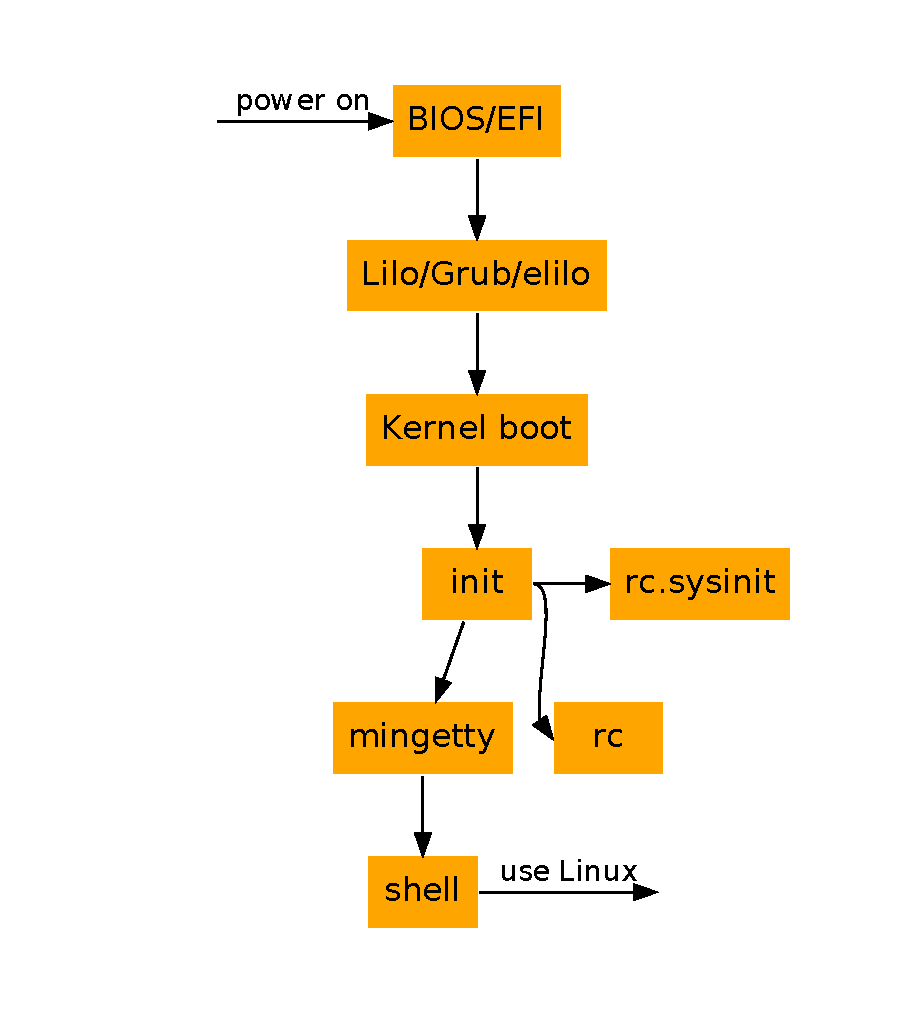
\includegraphics[height=.8\textheight]{images/boot.pdf}

%\begin{itemize}
%\item 加载器配置文件(/boot/grub/grub.conf)
%\item Kernel
%\item /sbin/init
%\item /etc/rc.d/rc.sysinit
%\item etc/rc.d/rc,/etc/rc.d/rc?.d/
%\item /etc/rc.d/rc.local
%\item X
%\end{itemize}
\end{frame}


\subsection{文件系统故障}



\begin{frame}{启动时的文件系统问题}
\begin{itemize}
\item rc.sysinit 尝试挂载本地文件系统
\item 如果失败,引导至root shell环境(需要输入密码)

\begin{itemize}
\item fsck 可以用来修复损坏的文件系统
\item 运行fsck之前

\begin{itemize}
\item 检查/etc/fstab是否有错误
\item 手工测试挂载文件系统
\end{itemize}
\end{itemize}
\end{itemize}

\end{frame} 
\begin{frame}{文件系统损坏}
\begin{itemize}
\item 一般系统崩溃或者非正常关机会导致文件系统损坏
\item 标记为`dirty'的ext2文件系统挂载时:

\begin{itemize}
\item 如果没有挂载或者只读挂载,标记为`clean'
\item 如果没有挂载且标记为`dirty',可能会报文件系统损坏
\item 需要彻底检查文件系统来进行修复
\end{itemize}
\item ext3通常标记为`clean'

\begin{itemize}
\item 如果需要恢复,日志(journal)会指出这点
\item 需要检查记录在日志里的文件
\end{itemize}
\end{itemize}

\end{frame} 
\begin{frame}{文件系统恢复}
\begin{itemize}
\item 如果 / 是日志文件系统,系统启动时检查它
\item /etc/rc.d/rc.sysinit 对/etc/fstab标记需要检查的文件系统做检查
\item fsck是其他文件系统检查工具的前端程序
\item fsck检查失效,则必须手工干预和执行
\end{itemize}

\end{frame} 
\begin{frame}{恢复运行级别}
\begin{itemize}
\item 传递运行级别(run-level)给init

\begin{itemize}
\item 在grub引导时传递参数
\item 在命令行下,使用init/telinit来改变
\end{itemize}
\item Runlevel 1

\begin{itemize}
\item 处理 rc.sysinit和rc1.d/目录下的脚本
\end{itemize}
\item Runlevel s/S/single

\begin{itemize}
\item 仅处理 rc.sysinit
\end{itemize}
\item emergency

\begin{itemize}
\item 仅处理sulogin
\end{itemize}
\end{itemize}
\end{frame} 

\subsection{救援环境}

\begin{frame}{救援环境}
\begin{itemize}
\item 当根文件系统失效时可以用到它
\item 非系统特性
\item 从第一张系统安装光盘启动,或者boot.iso
\item 如果是U盘,从diskboot.img启动
\item 引导后出现boot: 的地方,输入\alert{linux rescue}
\end{itemize}

\end{frame} 
\begin{frame}{工具}


\begin{itemize}
\item 磁盘维护工具
\item 网络工具
\item 其他一些工具
\item 记录日志: /tmp/syslog 或 /tmp/anaconda.log
\end{itemize}

\end{frame} 
\begin{frame}{细节}
\begin{itemize}
\item 文件系统重新组织

\begin{itemize}
\item anaconda 将会询问你是否需要挂载
\item /mnt/sysimage/{*}
\item /mnt/source
\item \$PATH 包括了磁盘的目录
\end{itemize}
\item 文件系统设备

\begin{itemize}
\item 提供特定文件系统设备
\item mknod可以创建已知主设备号和次设备号的设备
\end{itemize}
\end{itemize}
\end{frame} 


%\subsection{系统救援和故障排查实验}
%
%\begin{frame}{实验I:救援模式下修复GRUB}
%
%
%\begin{description}
%\item [{场景:}] 救援环境提供了修复机器不能启动的最后手段,即便引导器或者根文件系统损坏或者配置错误都可以修复。现在,有一台服务器在引导时,仅出现GR提示符,无法引导系统。请修复它。
%\end{description}
%提示
%\begin{itemize}
%\item 模拟MBR错误
%\item 第一张光盘引导,输入linux rescue
%\item 使用grub-install 指令
%\end{itemize}
%
%\end{frame} 
%
%\begin{frame}{实验II:救援模式下安装软件}
%
%
%\begin{description}
%\item [{场景:}] 因为文件系统的损坏,导致/bin/下的关键可执行程序损坏,包括/bin/mount,/bin/bash等。导致系统无法启动,请你修复该系统。
%\item [{要求:}] 修复损坏的RPM包
%\end{description}
%提示
%\begin{enumerate}
%\item 了解损坏的文件属于哪个RPM包
%\item 进入救援模式
%\item chroot环境
%\item 重新安装包
%\end{enumerate}
%\end{frame}

%\section{shell编程}

\begin{frame}{shell编程}
	\tableofcontents[currentsection]
\end{frame}

\subsection{shell 简介}
\begin{frame}{shell简介}
每一个操作系统都会有提供一个在命令行下用户和系统内核打交道的接口,一般我们称它为shell
\begin{itemize}
\item Windows Command Prompt(PowerShell)
\item sh 最原始的shell
	\begin{description}
	\item[bash] Bourne-Again Shell,来自sh的改进
	\item[ksh] Korn shell ,sh的超集
	\end{description}
\item csh C语言语法风格的shell
	\begin{description}
	\item[tcsh] csh的改进版本
	\end{description}
\item $\ldots$
\end{itemize}
\end{frame}

\begin{frame}{sh,bash 最广泛的脚本编程语言}
\begin{itemize}
\item shell = 命令执行的宏处理器
\item 直接调用Unix命令和内置的一些指令,在使用上,看不出区别
\item 完备的编程语言
\item 输入来源可以是:
	\begin{itemize}
	\item 来自终端
	\item 来自包含指令的文件
	\end{itemize}
\end{itemize}
\end{frame}

\subsection{bash 登录过程}

\begin{frame}[allowframebreaks]{bash登录过程}
\begin{itemize}
\item getty的程序负责等待用户登录,这就是我们在终端上看到的“login:”。 

\item  当用户输入用户名并回车后,getty进程将结束并启动login程序,即在终端显示字符串“password:”。

\item 接下来用户输入密码并回车,login将验证用户名密码是否与系统文件/etc/passwd中的记录以及/etc/shadow中的密码是否一致。 

\item 如果通过,则激活/etc/passwd中该用户记录行的最后一列的程序,如果没有设置,则启动/usr/bin/sh程序。

\item 这期间也将执行预定义好的用户环境脚本,这些初始化脚本执行结束后,终端将出现命令提示符等待用户输入命令,登录过程至此全部完成。 

\item 用户退出系统后,shell将退出,但系统会自动在该终端启动一个新的getty,等待用户登录。正如我们看到的好像“login:”永远不会消失一样。
\end{itemize}
\end{frame}

\subsection{bash如何执行启动脚本}

\begin{frame}[fragile,allowframebreaks]{bash如何执行它的启动文件}
\begin{block}{当bash是作为交互的登录 shell 启动的:}
\begin{verbatim} 
Login:root
Password:******
reading ~/.bash_login ... 
Last login: Thu May 26 10:26:56 2011 from 192.168.8.10
reading /etc/profile ... 
reading ~/.bashrc ... 
reading ~/.bash_profile ... 
[root@ ~]# 
\end{verbatim}
\end{block}

\begin{block}{以非交互式的 shell 指定 --login 选项启动的}
\begin{verbatim}
[root@ ~]# bash --login
reading /etc/profile ... 
reading ~/.bashrc ... 
reading ~/.bash_profile ... 
[root@ ~]# 
\end{verbatim}
\end{block}

\newpage

\begin{block}{以非交互式启动 shell }
\begin{verbatim}
[root@ ~]# bash
reading ~/.bashrc ... 
[root@ ~]# 
\end{verbatim}
\end{block}

\newpage

\begin{block}{如果 shell 是以与真实用户(组) id 不同的有效用户(组) id 来启动的, 并且没有 - 选项,那么它不会读取启动文件, 也不会从环境中继承 shell 函数. }
\begin{verbatim}
[root@ ~]# su 
reading ~/.bashrc ... 
[root@ ~]# su -
reading /etc/profile ... 
reading ~/.bashrc ... 
reading ~/.bash_profile ..
\end{verbatim}
\end{block}
\end{frame}

\begin{frame}{bash 保留字}
\begin{verbatim}
! case  do done elif else esac fi for function  
if in select then until while { } time [[ ]]
\end{verbatim}
\end{frame}

\subsection{bash 语法}

\begin{frame}[fragile,allowframebreaks]{bash 语法}
\begin{block}{Simple Commands}
\alert{Simple Commands 简单命令} 是一组词序列,第一个词定义为命令,它被成为第0个参数,其余词被作为这个命令的参数.
\end{block}

\newpage

\begin{block}{pipleline}
\alert{pipeline 管道} 是一组命令序列,用字符 | 分隔。管道的格式: 命令 command 的标准输出通过管道连接到命令 command2 的标准输入。连接是在命令指定的任何重定向之前进行的。

\begin{verbatim}
[root@ opt]# time ls -R |wc -l
50203

real    0m2.309s
user    0m0.178s
sys     0m0.341s
[root@ opt]#
\end{verbatim}
\end{block}

\begin{block}{命令序列}
\alert{序列} 序列是一个或多个管道,用操作符 ;, \&,\&\&, │, 或 <newline>新行符结束\begin{description}
\item[cmd1; cmd2; $\cdots$] 顺序执行
\item[cmd1 \&] 异步执行
\item[cmd1; \&\& cmd2 $\cdots$] 前一个命令执行成功才会执行后一个命令
\item[cmd1 || cmd2 ] cmd1返回非0值才会执行cmd2
\end{description}
\end{block}
\end{frame}


\begin{frame}[fragile,allowframebreaks]{复合命令}
\begin{block}{(command; command $\cdots$)}
( $ \cdots $ )将在一个子 shell 中执行。变量赋值和影响 shell 环境变量的内建命令在命令结束后不会再起作用。返回值是序列的返回值 \\
(ls) ;  (ls)
\end{block}

\newpage

\begin{block}{\{ commands; \} }
序列将在当前 shell 环境中执行。序列必须以一个新行符或分号结束。注意与元字符 ( 和 )不同, \{ 和 \} 是 reserved words(保留字),必须出现在能够识别保留字的场合。由于它们不会产生断词,它们和序列之间必须用空格分开。
\begin{verbatim}
#{ ls; }              //  wrong:  {ls}  {ls;}
#{ ls; } ; { df; }
\end{verbatim}
\end{block}

\newpage

\begin{block}{(( expression )) }
表 达 式 expression 赋值语句。如果表达式的值非零,返回值就是  0 ;否则返回值是 1。这种做法和 let “expression” 等价。
\begin{verbatim}
[root@ ~]# w=3; y=4; ((z=w+y)) ; echo $z
7
[root@ ~]# w=3; y=4; let z=w+y ; echo $z
7
\end{verbatim}
\end{block}

\newpage

\begin{block}{[[ expression ]] }
返回 0 或 1,取决于条件表达式 expression 求值的情况。表达式的原语组成稍后介绍;
\begin{verbatim}
[root@ ~]# [[ 3 != 3 ]] ; echo $?
1
[root@ ~]#  a="wer";[ $a = wer ]; echo $?
0
[root@ ~]# ((23>34)); echo $?
1
\end{verbatim}
\end{block}
\end{frame}

\subsection{bash 语句}

\begin{frame}[fragile,allowframebreaks,plain]{bash 语句}

\begin{block}{for name [ in word ] ; do list; done }
in 之后的一系列词会被扩展,产生一个项目列表。变量 name 被依次赋以这个列表中的每个元素,序列 list 每次都被执行。返回值是最后一个命令的返回值。
\begin{verbatim}
[root@~]# for i in a b c d;do echo $i; done
a
b
c
d
\end{verbatim}
\end{block}

\newpage

\begin{block}{for (( expr1; expr2; expr3 )); do list; done }
\begin{verbatim}
[root@~]# for (( i=0; i<10;i++ )); echo $i; done
0
1
2
3
...
8
9
\end{verbatim}
\end{block}

\newpage

\begin{block}{select name [ in word ]; do list; done}
\begin{verbatim}
#!/bin/bash
word="a b c"
select i in $word; do
	case $i in 
		a) echo "I am A"
		;;
		*) break
		;;
esac	
done
\end{verbatim}
\end{block}

\newpage

\begin{block}{执行结果}
\begin{verbatim}
[root@~]#./test.sh
./test.sh
1) a
2) b
3) c
#? 1
I am A
#? 2
\end{verbatim}
\end{block}

\newpage

\begin{block}{if条件语句}
\begin{verbatim}
if list; then
    list;
    [elif list; then list;]
    ...
    [else list; ]
fi
\end{verbatim}
\end{block}

\newpage

\begin{block}{loop \& function}
\begin{verbatim}
while list; do list; done
until list; do list; done
[ function ] name () {list;} 
name [ arg1,arg2,...]
\end{verbatim}
\end{block}
\end{frame}


\begin{frame}{特殊参数}
\begin{description}
\item [\$*] \$* 扩展为位置参数, “\$*” 等价于 “\$1c\$2c $\ldots$”, 这里 c 是变量 IFS 的第一个字符。如果没有设置 IFS,用空格分隔。
\item[\$@ ]等价于 "\$1" "\$2" $\ldots$
\item [\$\#] 扩展为位置参数的个数,以十进制表示。
\item [\$? ] 扩展为最近执行的前台管道的状态。
\item [\$\$] 扩展 为shell 的进程 ID。
\item [\$!] 扩展为最近一次执行的后台 (异步) 命令的进程号。
\item [\$0 ] 启动脚本名,或者指向通过bash -c 运行的第一个参数
\item [\$\_]  shell 启动时,设置为 shell 或参数中被执行的 shell 脚本的绝对路径名。
\end{description}
\end{frame}

\begin{frame}[allowframebreaks]{常用的shell变量}
\begin{description}
\item [HOSTNAME] 自动设置为当前的主机名
\item [OLDPWD] 上一次命令 cd 设置的工作目录
\item [HOSTTYPE] 标识当前脚本运行的机器类型 "x86\_64"
\item [PPID]  当前进程的父进程号,只读变量
\item [PWD]  当前工作目录
\item [SECONDS] 返回当前脚本自运行以来的秒数。如果向 SECONDS赋 值,此后对它的引用将返回自赋值时起的秒数加上所赋予的值。
\item [RANDOM] 每次引用这个参数,都会产生 0 到 32767 之间的随机整数
\item [UID] 当前用户的 ID,在启动时初始化。这个变量是只读的
\item [LANG] 用来决定没有特意用LC\_变量制定的语言环境项
\item [LC\_ALL] 这个变量超与了LANG和所有其他制定语言环境项的LC\_变量
\item [PATH] 搜索命令的路径,路径之间用冒号(:) 分隔
\item [TMOUT] 如果设置为大于 0 的值,TMOUT 被当作内建命令 read 的默认超时等待时间。如果等待终端输入时, TMOUT 秒之后仍然没有输入,bash 将退出.
\item [HISTFILE] 保存命令历史的文件名。默 认 值 \textasciitilde{}/.bash\_history 如果取消定义,在交互式 shell 退出时命令历史将不会保存
\item [HISTSIZE] 命令历史中保存的历史数量
\item [HOME] 当前用户的个人目录;内建命令 cd 的默认参数。波浪线扩展为此变量
\item [HOSTFILE] 包含一个格式和 /etc/hosts 相同的文件名。当 shell 需要补全主机名时要读取它
\end{description}
\end{frame}

\begin{frame}{Arrays 变量}
Bash  提供了一维数组变量。任何变量都可以作为一个数组 \\
要显式地 定义 一 个 数 组 ,使用 declare -a name。数组的大小没有上限,从 0 开始\\
如果变量赋值时使用语法 name[n]=value,会自动创建数组。\\
数组的任何元素都可以用 \$\{name[subscript]\} 来引用。花括号是必须的,以避免和路径扩展冲突。\\
如果 subscript 是 @ 或是 *,它扩展为 name 的所有成员。\\
这两种下标只有在双引号中才不同。在双引号中,\$\{name[*]\} 扩展为一个 词, 由所有数组成员的值组成,用特殊变量 IFS 的第一个字符分隔;\$\{name[@]\}将 name 的每个成员扩展为一个词
\end{frame}

\begin{frame}{命令行扩展}
Bash有 七 种 类 型的扩展:
\begin{enumerate}
\item brace expansion( 花 括 号 扩 展)
\item  tilde expansion(波浪线扩展)
\item parameter and variable expansion(参数和变量扩展)
\item command substitution(命令替换)
\item arithmetic  expansion(算术扩展)
\item  word splitting(词的拆分)
\item pathname expansion(路径扩展)
\end{enumerate}
例如, a\{d,c,b\}e 扩展为 ‘ade ace abe’。这种结构通常用来简写字符串的公共前缀较长的情况,例如 \\
mkdir /usr/local/src/bash/\{old,new,dist,bugs\} \\
chown root /usr/\{ucb/\{ex,edit\},lib/\{ex?.?*,how\_ex\}\}
\end{frame}

\begin{frame}{模式匹配}
\begin{description}
\item [ * ] 匹配任何字符串包括空串
\item [ ? ] 匹配任何一个字符
\item [ $\cdots$] 匹配所包含的任何字符之一 
\item [ - ] 范围表达式,任何排在他们之间的字符,都会被匹配
\end{description}
\end{frame}

%\begin{frame}{重定向}
%bash允许使用下面的几种结构将标准输入和标准错误输出重定向到用户定义的字符流中
%\begin{itemize}
%\item \&>word
%\item >\&word
%\item >word \&
%\item >word 2>\&1
%\end{itemize}
%\end{frame}

\begin{frame}[fragile]{Here Documents}
这种重定向使得shell从当前源文件中读取输入,知道遇到仅包含关键字的一行为止
\begin{verbatim}
#!/bin/sh
cat << EOF
     hello
    this is 
    here 
    documents
EOF 
\end{verbatim}
\href{http://blog.wgzhao.com/2009/08/24/here-documents-in-bash.html}{几种特别的用法}
\end{frame}

\begin{frame}[allowframebreaks]{条件表达式}
条件表达式用于 [[ ]]复合命令以及内建命令 test 和 [ ]中,用来测试文件属 性,进行字符串和算术比较
\begin{description}
\item [-a file] 如果 file 存在则为真
\item [-b file] 如果 file 存在且为块设备则为真
\item [-c file] 如果 file 存在且为字符设备则为真
\item [-d file] 如果 file 存在且是一个目录则为真
\item [-e file] 如果 file 存在则为真
\item [-f file] 如果 file 存在且为普通文件则为真
\item [-g file] 如果 file 存在且是设置组ID的 (sgid) 则为真
\item [-h file]  file 存在且为符号链接则为真
\item [-k file] 如果 file 存在且设置了 ‘‘sticky’’ 位 (粘滞位) 则为真
\item [-p file] 如果 file 存在且是一个命名管道 (FIFO) 则为真
\item [-r file] 如果 file 存在且可读则为真
\item [-s file] 如果 file 存在且大小大于零则为真
\item [-t fd] 如果文件描述符 fd 是打开的且对应一个终端则为真
\item [-u file] 如果 file 存在且是设置用户ID的 (suid) 则为真
\item [-w file]		如果 file 存在且可写则为真
\item [-x file]		如果 file 存在且可执行则为真
\item [-O file]		如果 file 存在且为有效用户ID所拥有则为真
\item [-G file]		如果 file 存在且为有效组ID所拥有则为真
\item [-L file]		如果 file 存在且为符号链接则为真
\item [-S file]		如果 file 存在且为套接字则为真
\item [-N file]		如果 file 存在且上次读取后被修改过则为真
\item [-z string] 如果string的长度为0 则为真
\item [-n string] 如果string的长度非0则为真

\item [file1 -nt file2] 如果 file1 比 file2 要新 (根据修改日期)则为真
\item [file1 -ot file2] 如果 file1 比 file2 更旧则为真
\item [file1 -ef file2]	如果 file1 和 file2 指的是相同得inode号则为真
\item [string1 == string2] 如果字符串相等则为真, = 可以用于使用==的场合来兼容POSIX规范
\item [string1 != string2] 如果字符串不相等则为真
\item [string1 < string2] 如果string1 在当前语言环境的字典顺序中排在string2之前则为真
\item [string1 > string2] 如果string1 在当前语言环境的字典顺序中排在string2之后则为真
\item [arg1 \underline{OP} arg2 ] OP 是 -eq, -ne, -lt, -le, -gt,-ge之一,这写算术操作返回真,如果arg1与args2分别是相等,不等,小于等于,大于,大于等于关系.arg1和arg2可以是正负整数.
\end{description}

\end{frame}

\subsection{grep}

\begin{frame}{grep}
grep (global search regular expression and print out the line)是一种强大的文本搜索工具,它能查找文件中指定的正则表达式,并打印含有该表达式的所有行。\\
使用grep的好处在于,不需要启动vi、ex等编辑器来执行查找,由于是命令行,又可以进行文件批量扫描查找,并且不需要将将正则表达式包含到斜线中
\end{frame}

\begin{frame}{grep常用参数}
\begin{description}
\item [-c ] 只输出匹配行的计数
\item [ -i ] 不分区大小写(只适用于单字符)
\item [ -l ] 只输出包含匹配字符的文件名
\item [ -n ] 显示匹配行及行号
\item [ -v ] 显示不包含匹配文本的所有行
\end{description}
\href{http://wangcong.org/blog/?p=1439}{http://wangcong.org/blog/?p=1439}
\end{frame}


\subsection{sed}

\begin{frame}[fragile,allowframebreaks]{sed}

\begin{block}{\alert{d} 删除命令}
\begin{itemize}
\item sed -e '1d' /etc/profile
\item sed -e '/\^\#/d' /etc/profile
\item sed -e '1,5d' /etc/profile
\end{itemize}
\end{block}

\begin{block}{\alert{s} 替换命令}
\begin{itemize}
\item sed 's/apple/orange/g' file
\item sed -n 's/\(new\) day/\textbackslash{}1 year/p' file 
\end{itemize}
\end{block}

\begin{block}{\alert{,} 行范围指定符}
\begin{itemize}
\item sed '/ifndef/,/endif/s/\$/END/' file \\
修改从ifndef到endif之间的所有行,并将各行末尾加上字符串END 
\item sed -e '/\#ifndef/,/\textbackslash{}\#endif/s/aaa/bbb/' prog.h
\end{itemize}
\end{block}

\begin{block}{\alert{a\textbackslash} 追加命令}
a\textbackslash 表示追加文本。注意a命令要以“\textbackslash{}” 结尾,追加内容将被加入匹配行的下一行 \\
\verb| sed '/^##/a\ this is an appended line ' file |

本例所做的操作是把所有以“\#\#”开头的行后面附加一行文本
\end{block}

\begin{block}{\alert{i\textbackslash}  插入命令}
i命令和a命令一样要以“\textbackslash" 结尾, 所不同的是, 它所追加的内容将被插入匹配行的前一行 \\
sed ‘/\^\#\# /i\textbackslash{} This is an inserted line’ file \\
本例所做的操作是把所有以“\#\#”加空格开头的行前面插入一行文本
\end{block}

\begin{block}{\alert{n} 下一行命令}
这个命令也很常用,很多系统配置文件的修改操作可以看到它。\\
sed '/Section \textbackslash{}"Device\textbackslash"{}/\{n;n;s/i810/vesa/;\}’ file \\
本例所做的操作是先找到以Section “Device”开始的行,找到后,对它的下面第二行中的i810替换为vesa
\end{block}

\begin{block}{sed单行脚本快速参考}

\href{http://sed.sourceforge.net/sed1line\_zh-CN.html}{http://sed.sourceforge.net/sed1line\_zh-CN.html}
\end{block}
\end{frame}

\subsection{awk}

\begin{frame}{awk}
\alert{awk} = \alert{A}ho \alert{W}einberger \alert{K}ernighan
\begin{quote}
Awk is a programming language designed to make many common information  retrieval  and text manipulation tasks  easy to state and to perform.
\end{quote}
\end{frame}

\begin{frame}{awk版本}
\begin{description}
\item[awk] Bell实验室的原始版本(Verion 7 UNIX, \textbackslash{} 1978) + 最新的POSIX awk 版本
\item[nawk] New awk,大约1989年随SVR4发布的版本
\item[gawk] awk的GNU组织实现版本,大部分Linux发行版本都有他.
\item[mawk] Michael的版本
\item[$\cdots$]
\end{description}
除了一些细微差别外,所有的这些发行版本功能基本相当.
\end{frame}

\begin{frame}{基本概念}
\begin{itemize}
\item awk 从文件或者标准输入读取,然后输出到标准输出
\item awk 识别 文件(file) , 记录(record) 和域(field)的概念
\item 文件有记录组成,缺省情况下,文件的每一行称为一条记录
\item awk 同一时刻只操作一条记录
\item 记录有一个或多个域组成,缺省情况下,域之间由空格或者制表符分隔(数目不限)
\item awk通过\${}1 访问第一个域,通过\${}2 访问第二个域,以此类推
\item 
\end{itemize}
\end{frame}

\begin{frame}{awk的基本结构}
\begin{itemize}
\item 一个awk语句或者脚本是下列语句的组合 \\
\alert{pattern}   \{ action \} \\
\alert{pattern}   \{ action \} \\
$\cdots$

\item \alert{pattern} 做为 action之否执行的一个判断
\item patterns 可以是:
	\begin{itemize}
		\item 正规表达式(regular expressions)
		\item 算术相关表达式
		\item 字符串值表达式
		\item 任意布尔值的组合
	\end{itemize}
\end{itemize}
\end{frame}

\begin{frame}[fragile]{一个简单的例子}
\begin{exampleblock}{需求}
从 \textbf{/etc/passwd} 文件获取用户 \textbf{wgzhao} 的用户ID号 \\
假设 /etc/passwd 文件由下面几行组成: \\
\begin{verbatim}
arun:x:504:504::/home/arun:/bin/bash
wgzhao:x:500:500::/home/wgzhao:/bin/bash
hacluster:x:501:501::/home/optima:/bin/bash
nfsbody:x:13:7::/var/lib:/sbin/nologin
\end{verbatim}

awk读取/etc/passwd文件,会认为:  \\
一行就是一个记录,因此这里共有4条记录 \\
一个记录由7个域组成,分隔符为":" (不是缺省分隔符)
\end{exampleblock}
\end{frame}

\begin{frame}{一个答案}
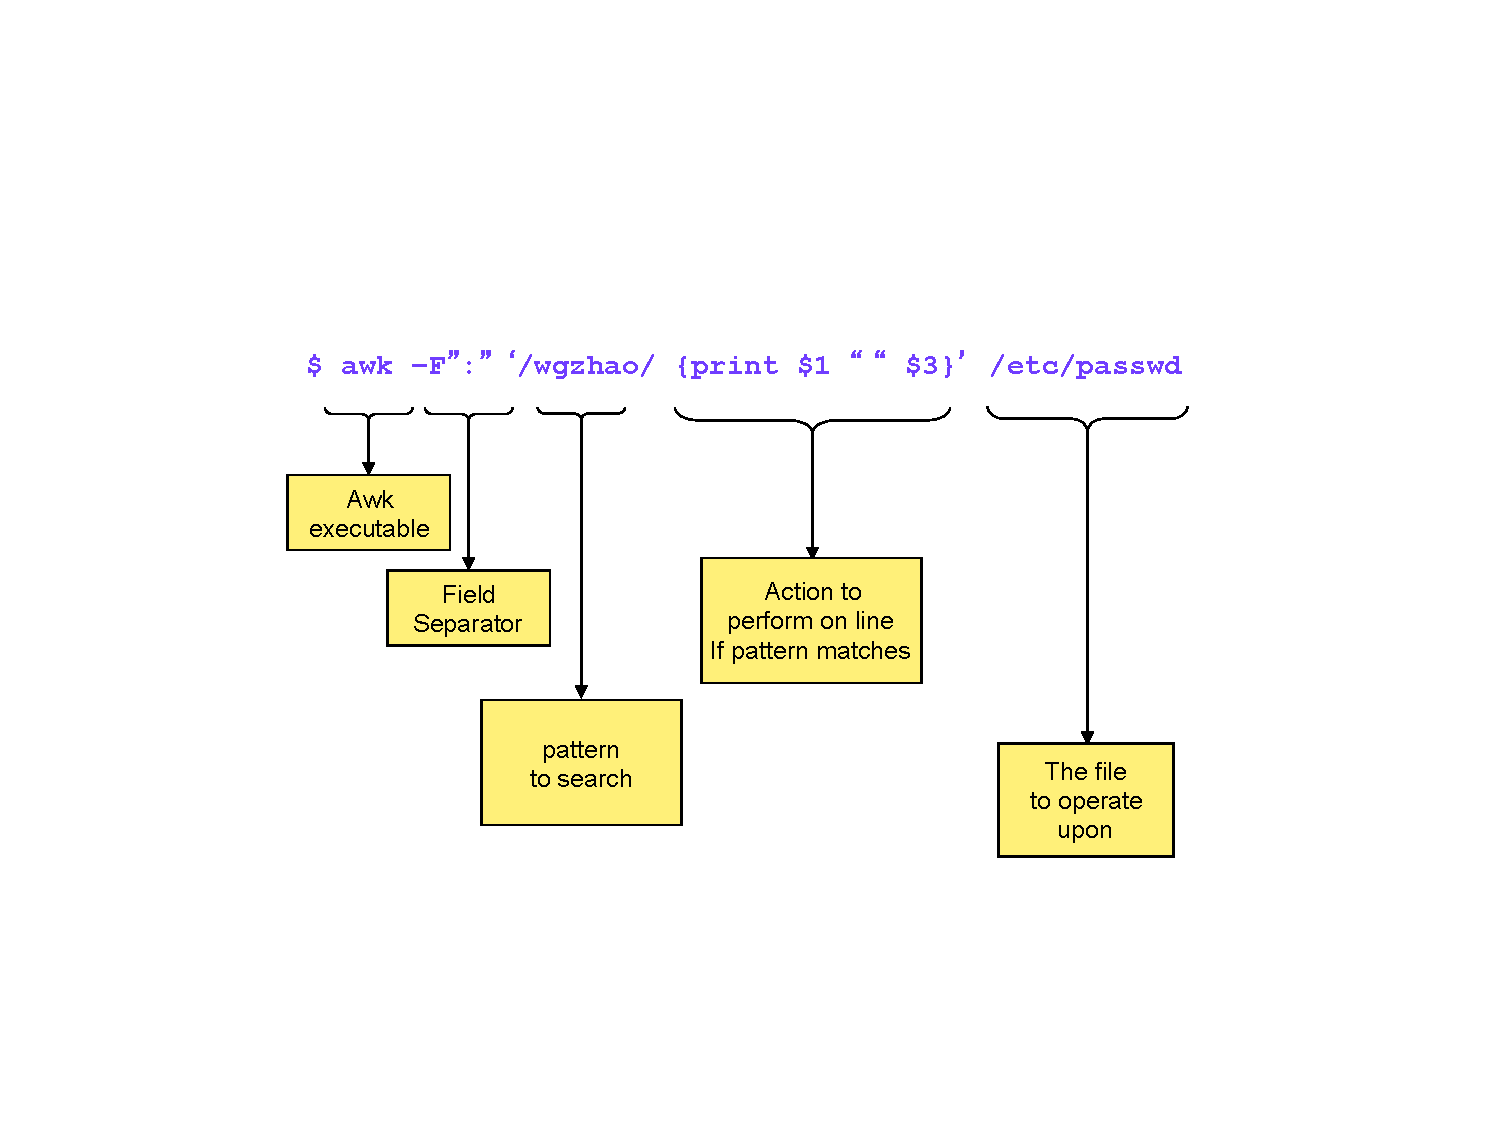
\includegraphics[scale=.6]{awk-example}
\end{frame}

\begin{frame}[fragile]{执行结果}
\begin{verbatim}
[root@~]# awk -F":" ‘/wgzhao/ {print $1 " " $3}’ /etc/passwd 
 wgzhao 500
\end{verbatim}

换一个写法
\begin{verbatim}
[root@ ~ ]# awk ‘BEGIN { FS=“:” } /arun/ {print $1 " " $3}’ /etc/passwd 
 wgzhao 500
\end{verbatim}
\end{frame}

\begin{frame}[fragile,allowframebreaks]{运行awk程序}
一般来说,我们有四种方式来运行awk程序
\begin{enumerate}
\item 单行脚本模式 \\
  e.g  awk 'program' input-file1 input-file2  $\cdots$
\item 没有输入文件,直接从终端读取 \\
\begin{verbatim}
$ awk 'program' <ENTER>
<input lines>
<input lines>
...
ctrl-d
\end{verbatim}
\item 将awk代码写入脚本,然后调用 \\
e.g  awk -f source-file input-file1 input-file2 $\cdots$

\item 制作成可执行脚本,类似shell脚本
\begin{verbatim}
#!/bin/awk -f 
# a simple awk program
/foo/ { print $1 }
\end{verbatim}
chmod +x hello \\
./hello file.txt
\end{enumerate}
\end{frame}

\begin{frame}[fragile,allowframebreaks]{高级awk特性}
\begin{itemize}
\item Awk 从C语言里借鉴了很多
\item if 循环, for 循环 和while 循环和C语言的结构相同
\item Awk的变量在内部当作字符串存储 \\
\begin{verbatim}
x = "1.01"
x = x + 1
print x
\end{verbatim}
\item awk 里的比较操作符有: "==","<",">","<=",">=","!=","~","!~"

\item "~" 表示匹配(matches),"!~"则表示不匹配

\item awk 里的算术操作符有: "+","-","/","*"
\item "\^" 是乘方运算 , "\%" 是模运算
\item 所有 C 操作符,比如"++","--","+=","-=","/=" 等在awk里也有效
\item awk 支持一维数组,可以存储字符串或数值
\end{itemize}
\end{frame}

\begin{frame}[fragile,allowframebreaks]{awk 实例}
\begin{block}{打印/etc/passwd的所有行}
\begin{verbatim}
$ awk '{ print $0 }' /etc/passwd
\end{verbatim}
\end{block}

\begin{block}{打印/etc/passwd所有行的第一列和第三列,分隔符为":"}
\begin{verbatim}
awk -F":" '{ print "username: " $1 "\t\tuid:" $3" }' /etc/passwd 
\end{verbatim}
\end{block}

\begin{block}{计算/etc/passwd文件里空白行数}
\begin{verbatim}
$ awk –f script1.awk /etc/passwd
  script1.awk
  BEGIN{ x=0 }# The BEGIN block is executed before processing the file
  /^$/ { x=x+1 } # For every null line increment the count
  END { print "I found " x " blank lines. :)" } #Executed at the end
\end{verbatim}
\end{block}

\begin{block}{修改记录分隔符的例子}
\begin{verbatim}
awk 'BEGIN { RS = "/" } ; { print $0 }' file1.txt
\end{verbatim}
RS = Record Separator ,缺省是"\textbackslash{}n",上述例子表示把记录分隔符修成"/",因此awk按照"/"符号来对file1.txt区分断行
\end{block}
\end{frame}

%\section {Linux哲学}
\begin{frame}{Linux哲学}
\pause
\begin{center}
\tikz[align=center]\node[draw,line width=6pt,rounded corners=8pt,inner sep=5mm] {\fontsize{35}{35}\selectfont K.I.S.S. \\ \\ \fontsize{20}{20}\selectfont Keep It Simple,Stupid};

\end{center}
\end{frame}


\begin{frame}{无名师的Linux心传}
\begin{center}
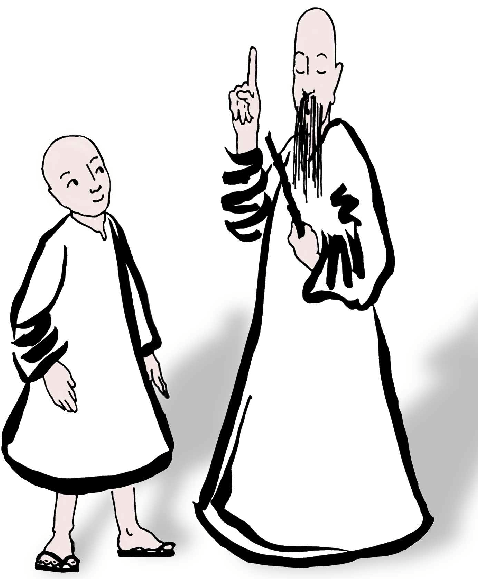
\includegraphics[height=0.7\textheight]{images/zen-linux.png} 
\end{center}
\end{frame}

\begin{frame}[shrink=5]{无名师与最终用户}
无名师又一次布道时,一个最终用户听说了他的智慧,跑来求 教。 他对无名师三鞠躬。\\
“我欲学习Unix大道,”他说,“但是弄不 懂命令行。”\\
 一个旁观的新门徒开始嘲讽最终用户,说他脑子一锅粥,说只有 训练有素、有智慧者才配适用Unix。 无名师抚手不语,命这个嘲笑最终用户的新门徒前坐,坐到最终 用户身边。 \\
 “告诉我,”他对新门徒说,“你写过什么代码,有过什么突出 设计。”\\
新门徒嗫嚅了两句,然后沉默了。 无名师转向最终用户。“告诉我”,他问,“为何你要寻求大 道?”\\
“我用的软件并不能令我满意”,最终用户答,“既不稳定,也 不美观。听说Unix之道尽管艰难,但超越一切,我愿抛去一切诱 饵和虚像。” \\
“那么,”无名师问,“你为何想尽办法让软件帮你做事?” \\
“我是一个建筑工”,最终用户答道,“这座城里的很多房屋都 出自我手。” \\
无名师转向新门徒。“家猫也能欺负老虎”,无名师说,“但是 猫叫永远比不过虎吼。” \\
听到此,新门徒眼中一亮。
\end{frame}

\begin{frame}[shrink]{无名师与Unix狂}
一个Unix狂热者听说无名师掌握Unix大道真理,便跑来求教。无 名师对他说: \\
“ 当尊者Thompson发明Unix时,他并不理解它。随后他理解了,受 益了,不再发明了。”  \\
“当尊者McIlroy发明管道时,他只知道他将传递软件,并不知 道他能传播思想。” \\
“当尊者Ritchie发明C时,他将程序员放到缓冲区溢出、堆损坏 和烂指针bug的地狱中惩罚。”\\
“说实话,这些尊者既瞎由蠢!” 狂热者堆无名师的用词极为愤怒。\\
 “这些智者”,他抗议到,“给了我们Unix的大道。我们嘲笑他 们,就是混淆是非,比转世为畜生和MCSE害不如。”\\
  “你的代码全无污点和缺陷?”无名师问。\\
   “不”,狂热者承认,“没人不犯错。”\\
   “这些尊者之智,”无名师说,“就是了解自身之愚。” 听到此,狂热者眼中一亮。
\end{frame}

\begin{frame}[allowframebreaks,allowdisplaybreaks]{无名师与脚本狂}
无名师和学生吃早饭时,从黑客大陆来了一个陌生访客。\\
 “I hear y00 are very 133t,”,他说。“P133z teach m3 all y00 know”。(我听说你很牛,请把你会的都教给我。) 无名师的学生面面相觑,都没有听懂这类粗鄙言语。\\
 无名师微笑 道:“你想弄懂Unix?” \\
 “I want to b3 a wizard hax0r”,陌生人回答,“and 0wn ever3one’s b0xen。”(我想当个顶尖黑客,能掌握所有人的 机器。) \\
 “我不教这个”,无名师答道。\\
  陌生人很激动。“D00d,y00r nothing but p0ser”,他说“If y00 m00 anything,y00 wud t33ch m3.”(哥们儿,感情你没 真本事呀,你要知道点儿东西就教给我了。) \\
  “有条路。”无名师说,“可以将你带入真知。”他在纸上写了 个IP地址。“黑掉这台机器,这对你来说应该不费什么力气,他 的管理员不称职。回来我告诉我你发现了什么。”\\
   陌生人鞠了一躬机离开了。无名师把他的早饭吃完。\\
    几天过去了,几个月过去了。每人再想起陌生人。\\
     数年过去了,黑客大陆来的陌生人回来了。 \\
     “你混蛋!”他说,“我黑掉了那台机器,你说的没错,太容易 了,但是我被FBI抓起来扔进监狱了。”\\
      “好”,无名师说,“你可以继续下一课了。”他在另一张纸上 写了个IP地址交给陌生人。 \\
      “你疯了?”陌生人喊道,“经过这事,我再也不黑别人的机器 了。”\\
       无名师脸露微笑。“这里就是”,他说,“真知的开始。”\\
        听到此,陌生人眼中一亮。
\end{frame}
%perferences
%提供一些学习Linux的途径,推荐的书籍,网络资源等
\section{深入学习的途径}
\begin{frame}{深入学习的途径}
\tableofcontents[currentsection]
\end{frame}

\subsection{推荐的书籍}
\begin{frame}{推荐的书籍}
\begin{itemize}
\item 《Linux系统管理员手册》(http://book.douban.com/subject/3042029)
\item 《学习Bash》(http://book.douban.com/subject/1241361/)
\item 《Advanced Bash-Scripting Guide》(http://www.tldp.org/LDP/abs/abs-guide.pdf)
\item 《sed与awk》(http://book.douban.com/subject/1236944/)
\item 《Linux设备驱动编程》(http://book.douban.com/subject/1723151/)
\item 《UNIX编程艺术》(http://book.douban.com/subject/1467587/)
\item 《UNIX环境高级编程》(http://book.douban.com/subject/1788421/)
\end{itemize}
\end{frame}

\subsection{推荐的网络资源}
\begin{frame}{推荐的网络资源}
\begin{itemize}
\item Google (NOT baidu)
\item Google(NOT baidu)
\itme Google(NOT baidu)
\item Red Hat Knowledge Base (http://kbase.redhat.com/faq)
\item Novell Support (http://support.novell.com/search/kb\_index.jsp)
\item Ubuntu Wiki (https://wiki.ubuntu.com/)
\item chinaunix forum (http://bbs.chinaunix.net/)
\item Linux info from the source (http://lwn.net/)
\item Kernel Trap (http://kerneltrap.org/)
\end{itemize}
\end{frame}

%thank you
\begin{frame}[plain]
\center 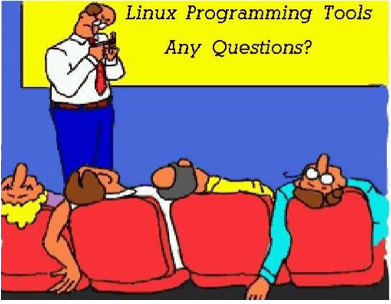
\includegraphics[width=.6\textwidth]{images/sleeping}
\end{frame}

\end{document}
